% !TeX program = xelatex
% !TeX encoding = UTF-8
\documentclass[UTF8,10pt,a4paper,fontset=fandol]{ctexart}
\usepackage{amsmath,amssymb,graphicx,tabularx,array,multirow,enumitem,titlesec,xcolor,ragged2e,etoolbox}
\usepackage[a4paper,top=1.6cm,bottom=1.6cm,left=1.6cm,right=1.6cm]{geometry}
\setlength{\parindent}{2em}
\setlength{\parskip}{0.15em}
\setlength{\tabcolsep}{4pt}
\renewcommand{\arraystretch}{1.15}
\setlist[enumerate]{leftmargin=2.6em,itemsep=0.1em,topsep=0.2em}
\titleformat{\section}{\large\bfseries}{\thesection}{0.6em}{}
\titleformat{\subsection}{\normalsize\bfseries}{\thesubsection}{0.6em}{}
\titleformat{\subsubsection}{\normalsize\bfseries}{\thesubsubsection}{0.6em}{}
\titlespacing*{\section}{0pt}{0.7em}{0.25em}
\titlespacing*{\subsection}{0pt}{0.55em}{0.2em}
\titlespacing*{\subsubsection}{0pt}{0.4em}{0.15em}
\raggedbottom
\BeforeBeginEnvironment{tabularx}{\par\noindent}
\newcommand{\fieldvalue}[1]{#1}
\newcommand{\handwritten}[1]{#1}
\newcommand{\checkboxfield}[1]{\ifstrequal{#1}{checked}{☑}{\ifstrequal{#1}{unclear}{?}{☐}}}
\begin{document}

\begin{center}
{\large\bfseries 艾米迈托赛普注射液放行检验}\\[0.3em]
\textbf{HBV、HCV 和 HIV（1/2）病原微生物检验}
\end{center}

\begin{tabular}{|p{0.14\linewidth}|p{0.36\linewidth}|p{0.14\linewidth}|p{0.28\linewidth}|}
\hline
样品名称 &
% #VALUE_ID: LEX-P0001-V0001
% #FIELD_VALUE: 样品名称
\fieldvalue{艾米迈托赛普注射液} &
样品规格 &
% #VALUE_ID: LEX-P0001-V0002
% #FIELD_VALUE: 样品规格
\fieldvalue{12 ml：$6.0\times10^{7}$ 个细胞}
\\ \hline
样品批号 &
% #VALUE_ID: LEX-P0001-V0003
% #FIELD_VALUE: 样品批号
% TODO #HANDWRITTEN: A?E?Z?10?0506; handwriting unclear
\fieldvalue{\handwritten{A?E?Z?10?0506}} &
取样日期 &
% #VALUE_ID: LEX-P0001-V0004
% #FIELD_VALUE: 取样日期
% TODO #HANDWRITTEN: 202?年8月?日; handwriting unclear
\fieldvalue{\handwritten{202?年8月?日}}
\\ \hline
\end{tabular}

\section*{1.\quad 仪器设备及试剂}

\subsection*{1.1.\quad 仪器设备}

\small
\begin{tabular}{|p{0.18\linewidth}|p{0.18\linewidth}|p{0.14\linewidth}|p{0.17\linewidth}|p{0.18\linewidth}|p{0.15\linewidth}|}
\hline
仪器名称 & 厂家 & 型号 & 设备编号 & 校准有效期至 & 状态是否完好\\ \hline
核酸提取仪 & 博日科技 & NPA-32E &
% #VALUE_ID: LEX-P0001-V0005
% #FIELD_VALUE: 核酸提取仪设备编号
% #HANDWRITTEN: 143?880
\fieldvalue{\handwritten{143?880}} &
% #VALUE_ID: LEX-P0001-V0006
% #FIELD_VALUE: 核酸提取仪校准有效期
% #HANDWRITTEN: 2026.06.09
\fieldvalue{\handwritten{2026.06.09}} &
是
% #VALUE_ID: LEX-P0001-V0007
% #FIELD_VALUE: 核酸提取仪状态“是”
% #HANDWRITTEN: ✓
\fieldvalue{\handwritten{\checkboxfield{checked}}}\quad否
% #VALUE_ID: LEX-P0001-V0008
% #FIELD_VALUE: 核酸提取仪状态“否”
\fieldvalue{\checkboxfield{unchecked}}
\\ \hline
实时荧光定量 PCR 仪 & Thermo & 7500 &
% #VALUE_ID: LEX-P0001-V0009
% #FIELD_VALUE: 实时荧光定量 PCR 仪设备编号
% #HANDWRITTEN: 141?71
\fieldvalue{\handwritten{141?71}} &
% #VALUE_ID: LEX-P0001-V0010
% #FIELD_VALUE: 实时荧光定量 PCR 仪校准有效期
% #HANDWRITTEN: 2026.06.04
\fieldvalue{\handwritten{2026.06.04}} &
是
% #VALUE_ID: LEX-P0001-V0011
% #FIELD_VALUE: 实时荧光定量 PCR 仪状态“是”
% #HANDWRITTEN: ✓
\fieldvalue{\handwritten{\checkboxfield{checked}}}\quad否
% #VALUE_ID: LEX-P0001-V0012
% #FIELD_VALUE: 实时荧光定量 PCR 仪状态“否”
\fieldvalue{\checkboxfield{unchecked}}
\\ \hline
生物安全柜 & Thermo & 1384 &
% #VALUE_ID: LEX-P0001-V0013
% #FIELD_VALUE: 生物安全柜设备编号
% #HANDWRITTEN: 10?2705
\fieldvalue{\handwritten{10?2705}} &
% #VALUE_ID: LEX-P0001-V0014
% #FIELD_VALUE: 生物安全柜校准有效期
% #HANDWRITTEN: 2026.06.09
\fieldvalue{\handwritten{2026.06.09}} &
是
% #VALUE_ID: LEX-P0001-V0015
% #FIELD_VALUE: 生物安全柜状态“是”
% #HANDWRITTEN: ✓
\fieldvalue{\handwritten{\checkboxfield{checked}}}\quad否
% #VALUE_ID: LEX-P0001-V0016
% #FIELD_VALUE: 生物安全柜状态“否”
\fieldvalue{\checkboxfield{unchecked}}
\\ \hline
\multirow{5}{*}{移液器} & \multirow{5}{*}{Eppendorf} &
% #VALUE_ID: LEX-P0001-V0017
% #FIELD_VALUE: 移液器型号
% #HANDWRITTEN: 10--200\,\textmu l
\fieldvalue{\handwritten{10--200\,\textmu l}} &
% #VALUE_ID: LEX-P0001-V0022
% #FIELD_VALUE: 移液器设备编号
% #HANDWRITTEN: P?2?7?
\fieldvalue{\handwritten{P?2?7?}} &
% #VALUE_ID: LEX-P0001-V0027
% #FIELD_VALUE: 移液器校准有效期
% #HANDWRITTEN: 2026.07.03
\fieldvalue{\handwritten{2026.07.03}} &
\multirow{5}{*}{是
% #VALUE_ID: LEX-P0001-V0032
% #FIELD_VALUE: 移液器状态“是”
% #HANDWRITTEN: ✓
\fieldvalue{\handwritten{\checkboxfield{checked}}}\quad否
% #VALUE_ID: LEX-P0001-V0033
% #FIELD_VALUE: 移液器状态“否”
\fieldvalue{\checkboxfield{unchecked}}}
\\ \cline{3-5}
& & 
% #VALUE_ID: LEX-P0001-V0018
% #FIELD_VALUE: 移液器型号
% #HANDWRITTEN: 10--1000\,\textmu l
\fieldvalue{\handwritten{10--1000\,\textmu l}} &
% #VALUE_ID: LEX-P0001-V0023
% #FIELD_VALUE: 移液器设备编号
% #HANDWRITTEN: B?8?9?
\fieldvalue{\handwritten{B?8?9?}} &
% #VALUE_ID: LEX-P0001-V0028
% #FIELD_VALUE: 移液器校准有效期
% #HANDWRITTEN: 2026.07.03
\fieldvalue{\handwritten{2026.07.03}} & \\ \cline{3-5}
& &
% #VALUE_ID: LEX-P0001-V0019
% #FIELD_VALUE: 移液器型号
% #HANDWRITTEN: 20--200\,\textmu l
\fieldvalue{\handwritten{20--200\,\textmu l}} &
% #VALUE_ID: LEX-P0001-V0024
% #FIELD_VALUE: 移液器设备编号
% #HANDWRITTEN: D?9?6?
\fieldvalue{\handwritten{D?9?6?}} &
% #VALUE_ID: LEX-P0001-V0029
% #FIELD_VALUE: 移液器校准有效期
% #HANDWRITTEN: 2026.07.03
\fieldvalue{\handwritten{2026.07.03}} & \\ \cline{3-5}
& &
% #VALUE_ID: LEX-P0001-V0020
% #FIELD_VALUE: 移液器型号
% #HANDWRITTEN: 20--200\,\textmu l
\fieldvalue{\handwritten{20--200\,\textmu l}} &
% #VALUE_ID: LEX-P0001-V0025
% #FIELD_VALUE: 移液器设备编号
% #HANDWRITTEN: D?4?0?
\fieldvalue{\handwritten{D?4?0?}} &
% #VALUE_ID: LEX-P0001-V0030
% #FIELD_VALUE: 移液器校准有效期
% #HANDWRITTEN: 2026.07.03
\fieldvalue{\handwritten{2026.07.03}} & \\ \cline{3-5}
& &
% #VALUE_ID: LEX-P0001-V0021
% #FIELD_VALUE: 移液器型号
% #HANDWRITTEN: 100--1000\,\textmu l
\fieldvalue{\handwritten{100--1000\,\textmu l}} &
% #VALUE_ID: LEX-P0001-V0026
% #FIELD_VALUE: 移液器设备编号
% #HANDWRITTEN: P?4?0?
\fieldvalue{\handwritten{P?4?0?}} &
% #VALUE_ID: LEX-P0001-V0031
% #FIELD_VALUE: 移液器校准有效期
% #HANDWRITTEN: 2026.07.03
\fieldvalue{\handwritten{2026.07.03}} & \\ \hline
\end{tabular}
\normalsize

\subsection*{1.2.\quad 试剂}

\begin{tabular}{|p{0.39\linewidth}|p{0.15\linewidth}|p{0.15\linewidth}|p{0.16\linewidth}|p{0.15\linewidth}|}
\hline
试剂名称 & 厂家 & 货号 & 批号 & 有效期至 \\ \hline
乙型肝炎病毒、丙型肝炎病毒、人类免疫缺陷病毒（1/2 型）核酸检测试剂盒（PCR-荧光法）
& 万泰生物 &
% #VALUE_ID: LEX-P0001-V0034
% #FIELD_VALUE: 货号
% #HANDWRITTEN: --
\fieldvalue{\handwritten{--}} &
% #VALUE_ID: LEX-P0001-V0035
% #FIELD_VALUE: 批号
% #HANDWRITTEN: B?3?5?0? 081
\fieldvalue{\handwritten{B?3?5?0? 081}} &
% #VALUE_ID: LEX-P0001-V0036
% #FIELD_VALUE: 有效期至
% #HANDWRITTEN: 2026.06.15
\fieldvalue{\handwritten{2026.06.15}}
\\ \hline
PBS & Vivacell & C3580-0500 &
% #VALUE_ID: LEX-P0001-V0037
% #FIELD_VALUE: PBS 批号
% #HANDWRITTEN: 24P?316
\fieldvalue{\handwritten{24P?316}} &
% #VALUE_ID: LEX-P0001-V0038
% #FIELD_VALUE: PBS 有效期至
% #HANDWRITTEN: 2026/10/?
\fieldvalue{\handwritten{2026/10/?}}
\\ \hline
\end{tabular}

\section*{2.\quad 操作步骤}

\begin{tabular}{|p{0.30\linewidth}|p{0.34\linewidth}|p{0.28\linewidth}|}
\hline
\multicolumn{3}{c}{溶液配制}\\ \hline
LH Buffer（ml） & 内标溶液（\textmu l） & 终体积（ml）\\ \hline
% #VALUE_ID: LEX-P0001-V0039
% #FIELD_VALUE: LH Buffer 体积
% #HANDWRITTEN: 14
\fieldvalue{\handwritten{14}} &
% #VALUE_ID: LEX-P0001-V0040
% #FIELD_VALUE: 内标溶液体积
% #HANDWRITTEN: 2
\fieldvalue{\handwritten{2}} &
% #VALUE_ID: LEX-P0001-V0041
% #FIELD_VALUE: 终体积
% #HANDWRITTEN: 140.28
\fieldvalue{\handwritten{140.28}}
\\ \hline
\multicolumn{3}{c}{DNA 抽提}\\ \hline
\begin{minipage}[t]{\linewidth}
待测样品准备：将供试品细胞悬液使用 PBS 稀释至
$2\times10^{5}$ cells/ml 的细胞悬液作为待测样品，配制 2 份。
\end{minipage}
&
\begin{minipage}[t]{\linewidth}
供试品密度：
% #VALUE_ID: LEX-P0001-V0042
% #FIELD_VALUE: 供试品密度
% #HANDWRITTEN: 1$\times10^{6}$
\fieldvalue{\handwritten{$1\times10^{6}$}}\ cells/ml

取供试品体积
% #VALUE_ID: LEX-P0001-V0043
% #FIELD_VALUE: 取供试品体积
% #HANDWRITTEN: 400
\fieldvalue{\handwritten{400}}\,\textmu l

PBS 体积
% #VALUE_ID: LEX-P0001-V0044
% #FIELD_VALUE: PBS 体积
% #HANDWRITTEN: 100
\fieldvalue{\handwritten{100}}\,\textmu l

细胞数为
% #VALUE_ID: LEX-P0001-V0045
% #FIELD_VALUE: 细胞数
% #HANDWRITTEN: 2$\times10^{5}$
\fieldvalue{\handwritten{$2\times10^{5}$}}\ cells/ml
\end{minipage}
&
\\ \hline
\begin{minipage}[t]{\linewidth}
阳性对照（BC1）样品、阳性对照（HIV-2）样品和阴性对照样品准备：取 250\textmu l 试剂盒自带的阳性对照（BC1）、阳性对照（HIV-2）和阴性对照分别与 750\textmu l PBS 混匀。
\end{minipage}
&
\begin{minipage}[t]{\linewidth}
试剂盒自带的阳性对照（BC1）、阳性对照（HIV-2）和阴性对照
\\
阳性对照体积
% #VALUE_ID: LEX-P0001-V0046
% #FIELD_VALUE: 阳性对照体积
% #HANDWRITTEN: 250
\fieldvalue{\handwritten{250}}\,\textmu l

PBS 补充体积
% #VALUE_ID: LEX-P0001-V0047
% #FIELD_VALUE: PBS 补充体积
% #HANDWRITTEN: 750
\fieldvalue{\handwritten{750}}\,\textmu l
\end{minipage}
&
\\ \hline
\end{tabular}

\vfill
\begin{center}
第 53 页\quad 共 73 页
\end{center}

% TODO: This page contains the visible continuation of a larger controlled document; only the content visible on this page is rendered.
% LEXOID_PAGE_COMPLETED: 1/81

\newpage

\begin{center}
\textbf{阳性生物制品（原）件}\\
文件编号：REC-YZ-SOP-QC-C3-092
\end{center}

\begin{tabular}{|p{0.43\linewidth}|p{0.47\linewidth}|}
\hline
取 $960\,\mu l$ 的待测样品（BC11样品）、阳性对照（BC11）样品、阴性对照（HIV-2）样品和阴性对照样品各 $40\,\mu l$ 蛋白酶 K 混合，再室温放置 $15\,\mathrm{min}$，备用。 &
待测样品、阳性对照（BC11）样品体积：
% #VALUE_ID: LEX-P0002-V0001
% #FIELD_VALUE: 阳性对照（BC11）样品体积
% #HANDWRITTEN: 160
\fieldvalue{\handwritten{160}} $\mu l$

2）阴性对照（HIV-2）样品体积：
% #VALUE_ID: LEX-P0002-V0002
% #FIELD_VALUE: 阴性对照（HIV-2）样品体积
% #HANDWRITTEN: 160
\fieldvalue{\handwritten{160}} $\mu l$

蛋白酶 K 体积：
% #VALUE_ID: LEX-P0002-V0003
% #FIELD_VALUE: 蛋白酶 K 体积
% #HANDWRITTEN: 60
\fieldvalue{\handwritten{60}} $\mu l$

孵育时间：
% #VALUE_ID: LEX-P0002-V0004
% #FIELD_VALUE: 孵育时间
% #HANDWRITTEN: 15
\fieldvalue{\handwritten{15}}\,\mathrm{min}
\\
\hline
取 $96$ 孔深孔板，进行试剂添加：

（a）向第 1 和第 2 列加入 $480\,\mu l$ 凝聚工作液；

（b）向第 3 列加入 $40\,\mu l$ Bictex；

（c）向第 3 列加入 $500\,\mu l$ Wash Buffer A；

（d）向第 4 列加入 $500\,\mu l$ Wash Buffer B；

（e）向第 5 列加入 $500\,\mu l$ W/E Buffer &
（a）向第 1 和第 2 列加入
% #VALUE_ID: LEX-P0002-V0005
% #FIELD_VALUE: 凝聚工作液体积
% #HANDWRITTEN: 480
\fieldvalue{\handwritten{480}} $\mu l$ 凝聚工作液；

（b）向第 3 列加入
% #VALUE_ID: LEX-P0002-V0006
% #FIELD_VALUE: Bictex 体积
% #HANDWRITTEN: 60
\fieldvalue{\handwritten{60}} $\mu l$ Bictex；

（c）向第 3 列加入
% #VALUE_ID: LEX-P0002-V0007
% #FIELD_VALUE: Wash Buffer A 体积
% #HANDWRITTEN: 500
\fieldvalue{\handwritten{500}} $\mu l$ Wash Buffer A；

（d）向第 4 列加入
% #VALUE_ID: LEX-P0002-V0008
% #FIELD_VALUE: Wash Buffer B 体积
% #HANDWRITTEN: 500
\fieldvalue{\handwritten{500}} $\mu l$ Wash Buffer B；

（e）向第 5 列加入
% #VALUE_ID: LEX-P0002-V0009
% #FIELD_VALUE: W/E Buffer 体积
% #HANDWRITTEN: 60
\fieldvalue{\handwritten{60}} $\mu l$ W/E Buffer
\\
\hline
第 1 和第 2 列各加入 $480\,\mu l$ 蛋白酶 K 处理后的待测样品、阳性对照（BC11）样品、阴性对照（HIV-2）样品和阴性对照样品。 &
加入蛋白酶 K 处理后各样品体积：
% #VALUE_ID: LEX-P0002-V0010
% #FIELD_VALUE: 蛋白酶 K 处理后各样品体积
% #HANDWRITTEN: 800
\fieldvalue{\handwritten{800}} $\mu l$
\\
\hline
\multicolumn{2}{|l|}{运行提取程序进行核酸提取，程序设置如下：}\\
\hline
（a）使用磁珠套条将第 1 和第 2 列各慢混匀 $10\,\mathrm{min}$； &
是\quad
% #VALUE_ID: LEX-P0002-V0011
% #FIELD_VALUE: （a）是
% #HANDWRITTEN: ✓
\fieldvalue{\handwritten{\checkboxfield{checked}}}
\quad 否\quad
% #VALUE_ID: LEX-P0002-V0012
% #FIELD_VALUE: （a）否
\fieldvalue{\checkboxfield{unchecked}}
\\
\hline
（b）Bictex（第 3 列）磁吸 $2.5\,\mathrm{min}$； &
是\quad
% #VALUE_ID: LEX-P0002-V0013
% #FIELD_VALUE: （b）是
% #HANDWRITTEN: ✓
\fieldvalue{\handwritten{\checkboxfield{checked}}}
\quad 否\quad
% #VALUE_ID: LEX-P0002-V0014
% #FIELD_VALUE: （b）否
\fieldvalue{\checkboxfield{unchecked}}
\\
\hline
（c）将磁珠依次转移第 1 和第 2 列，分别混匀 $5\,\mathrm{min}$ 和磁吸附 $2.5\,\mathrm{min}$； &
是\quad
% #VALUE_ID: LEX-P0002-V0015
% #FIELD_VALUE: （c）是
% #HANDWRITTEN: ✓
\fieldvalue{\handwritten{\checkboxfield{checked}}}
\quad 否\quad
% #VALUE_ID: LEX-P0002-V0016
% #FIELD_VALUE: （c）否
\fieldvalue{\checkboxfield{unchecked}}
\\
\hline
（d）Wash Buffer A（第 3 列）洗涤 $5\,\mathrm{min}$，磁吸附 $2.5\,\mathrm{min}$； &
是\quad
% #VALUE_ID: LEX-P0002-V0017
% #FIELD_VALUE: （d）是
% #HANDWRITTEN: ✓
\fieldvalue{\handwritten{\checkboxfield{checked}}}
\quad 否\quad
% #VALUE_ID: LEX-P0002-V0018
% #FIELD_VALUE: （d）否
\fieldvalue{\checkboxfield{unchecked}}
\\
\hline
（e）Wash Buffer B（第 4 列）洗涤 $2\,\mathrm{min}$，磁吸附 $2.5\,\mathrm{min}$，晾干 $7\,\mathrm{min}$； &
是\quad
% #VALUE_ID: LEX-P0002-V0019
% #FIELD_VALUE: （e）是
% #HANDWRITTEN: ✓
\fieldvalue{\handwritten{\checkboxfield{checked}}}
\quad 否\quad
% #VALUE_ID: LEX-P0002-V0020
% #FIELD_VALUE: （e）否
\fieldvalue{\checkboxfield{unchecked}}
\\
\hline
（f）W/E Buffer（第 5 列）洗脱 $2\,\mathrm{min}$，磁吸后 $55^\circ\mathrm{C}$。 &
是\quad
% #VALUE_ID: LEX-P0002-V0021
% #FIELD_VALUE: （f）是
% #HANDWRITTEN: ✓
\fieldvalue{\handwritten{\checkboxfield{checked}}}
\quad 否\quad
% #VALUE_ID: LEX-P0002-V0022
% #FIELD_VALUE: （f）否
\fieldvalue{\checkboxfield{unchecked}}
\\
\hline
（g）将磁珠移动至第 3 列弃除。 &
是\quad
% #VALUE_ID: LEX-P0002-V0023
% #FIELD_VALUE: （g）是
% #HANDWRITTEN: ✓
\fieldvalue{\handwritten{\checkboxfield{checked}}}
\quad 否\quad
% #VALUE_ID: LEX-P0002-V0024
% #FIELD_VALUE: （g）否
\fieldvalue{\checkboxfield{unchecked}}
\\
\hline
\multicolumn{2}{|c|}{\textbf{qPCR 反应制备}}\\
\hline
PCR 反应体系 & 添加量（$\mu l$）\\
\hline
RT-PCR 反应液 &
% #VALUE_ID: LEX-P0002-V0025
% #FIELD_VALUE: RT-PCR 反应液添加量
% #HANDWRITTEN: 37.5
\fieldvalue{\handwritten{37.5}}
\\
\hline
Mn(OAc)$_2$ &
% #VALUE_ID: LEX-P0002-V0026
% #FIELD_VALUE: Mn(OAc)$_2$ 添加量
% #HANDWRITTEN: 37.5
\fieldvalue{\handwritten{37.5}}
\\
\hline
引物探针 &
% #VALUE_ID: LEX-P0002-V0027
% #FIELD_VALUE: 引物探针添加量
% #HANDWRITTEN: 37.5
\fieldvalue{\handwritten{37.5}}
\\
\hline
反应管加入混合液体积 &
% #VALUE_ID: LEX-P0002-V0028
% #FIELD_VALUE: 反应管加入混合液体积
% #HANDWRITTEN: 20
\fieldvalue{\handwritten{20}}
\\
\hline
\multicolumn{2}{|c|}{\textbf{qPCR 扩增（扩增与分析区）}}\\
\hline
扩增探针设置 & \\
\hline
\end{tabular}
% LEXOID_PAGE_COMPLETED: 2/81

\newpage

\begin{center}
\textbf{PCR 反应体系及扩增程序记录}
\end{center}

\begin{tabular}{|p{0.07\linewidth}|p{0.19\linewidth}|p{0.19\linewidth}|p{0.19\linewidth}|p{0.20\linewidth}|}
\hline
序号 & Target & Reporter Dye & Quencher Dye & Passive Reference \\
\hline
1 &
% #VALUE_ID: LEX-P0003-V0001
% #FIELD_VALUE: Target 1
% #HANDWRITTEN: HBV
\fieldvalue{\handwritten{HBV}} &
% #VALUE_ID: LEX-P0003-V0002
% #FIELD_VALUE: Reporter Dye 1
% #HANDWRITTEN: ROX
\fieldvalue{\handwritten{ROX}} &
% #VALUE_ID: LEX-P0003-V0003
% #FIELD_VALUE: Quencher Dye 1
% #HANDWRITTEN: None
\fieldvalue{\handwritten{None}} &
\multirow{4}{*}{
% #VALUE_ID: LEX-P0004-V0013
% #FIELD_VALUE: Passive Reference
% #HANDWRITTEN: None
\fieldvalue{\handwritten{None}}}\\[-2mm]
\cline{1-4}
2 &
% #VALUE_ID: LEX-P0003-V0004
% #FIELD_VALUE: Target 2
% #HANDWRITTEN: HCV
\fieldvalue{\handwritten{HCV}} &
% #VALUE_ID: LEX-P0003-V0005
% #FIELD_VALUE: Reporter Dye 2
% #HANDWRITTEN: FAM
\fieldvalue{\handwritten{FAM}} &
% #VALUE_ID: LEX-P0003-V0006
% #FIELD_VALUE: Quencher Dye 2
% #HANDWRITTEN: None
\fieldvalue{\handwritten{None}} &
\\
\cline{1-4}
3 &
% #VALUE_ID: LEX-P0003-V0007
% #FIELD_VALUE: Target 3
% #HANDWRITTEN: HIV
\fieldvalue{\handwritten{HIV}} &
% #VALUE_ID: LEX-P0003-V0008
% #FIELD_VALUE: Reporter Dye 3
% #HANDWRITTEN: Cy5
\fieldvalue{\handwritten{Cy5}} &
% #VALUE_ID: LEX-P0003-V0009
% #FIELD_VALUE: Quencher Dye 3
% #HANDWRITTEN: None
\fieldvalue{\handwritten{None}} &
\\
\cline{1-4}
4 &
% #VALUE_ID: LEX-P0003-V0010
% #FIELD_VALUE: Target 4
% #HANDWRITTEN: IPC
\fieldvalue{\handwritten{IPC}} &
% #VALUE_ID: LEX-P0003-V0011
% #FIELD_VALUE: Reporter Dye 4
% #HANDWRITTEN: VIC
\fieldvalue{\handwritten{VIC}} &
% #VALUE_ID: LEX-P0003-V0012
% #FIELD_VALUE: Quencher Dye 4
% #HANDWRITTEN: None
\fieldvalue{\handwritten{None}} &
\\
\hline
\end{tabular}

\vspace{2mm}
\textbf{扩增程序设置}

\begin{tabular}{|p{0.08\linewidth}|p{0.28\linewidth}|p{0.20\linewidth}|p{0.22\linewidth}|p{0.15\linewidth}|}
\hline
Stage & Step & Temp & Duration & Cycle \\
\hline
1 & UNG 酶变性 &
% #VALUE_ID: LEX-P0003-V0014
% #FIELD_VALUE: Stage 1 temperature
% #HANDWRITTEN: 37
\fieldvalue{\handwritten{37}}(37)$^\circ$C &
% #VALUE_ID: LEX-P0003-V0015
% #FIELD_VALUE: Stage 1 duration
% #HANDWRITTEN: 2
\fieldvalue{\handwritten{2}}(2)min &
% #VALUE_ID: LEX-P0003-V0016
% #FIELD_VALUE: Stage 1 cycle
% #HANDWRITTEN: 1
\fieldvalue{\handwritten{1}}(1) \\
\hline
2 & RNA 变性 &
% #VALUE_ID: LEX-P0003-V0017
% #FIELD_VALUE: Stage 2 temperature
% #HANDWRITTEN: 93
\fieldvalue{\handwritten{93}}(93)$^\circ$C &
% #VALUE_ID: LEX-P0003-V0018
% #FIELD_VALUE: Stage 2 duration
% #HANDWRITTEN: 1
\fieldvalue{\handwritten{1}}(1)min &
% #VALUE_ID: LEX-P0003-V0019
% #FIELD_VALUE: Stage 2 cycle
% #HANDWRITTEN: 1
\fieldvalue{\handwritten{1}}(1) \\
\hline
3 & RNA 反转录 &
% #VALUE_ID: LEX-P0003-V0020
% #FIELD_VALUE: Stage 3 temperature
% #HANDWRITTEN: 61
\fieldvalue{\handwritten{61}}(61)$^\circ$C &
% #VALUE_ID: LEX-P0003-V0021
% #FIELD_VALUE: Stage 3 duration
% #HANDWRITTEN: 15
\fieldvalue{\handwritten{15}}(15)min &
% #VALUE_ID: LEX-P0003-V0022
% #FIELD_VALUE: Stage 3 cycle
% #HANDWRITTEN: 1
\fieldvalue{\handwritten{1}}(1) \\
\hline
4 & RNA 变性 &
% #VALUE_ID: LEX-P0003-V0023
% #FIELD_VALUE: Stage 4 temperature
% #HANDWRITTEN: 93
\fieldvalue{\handwritten{93}}(93)$^\circ$C &
% #VALUE_ID: LEX-P0003-V0024
% #FIELD_VALUE: Stage 4 duration
% #HANDWRITTEN: 1
\fieldvalue{\handwritten{1}}(1)min &
% #VALUE_ID: LEX-P0003-V0025
% #FIELD_VALUE: Stage 4 cycle
% #HANDWRITTEN: 1
\fieldvalue{\handwritten{1}}(1) \\
\hline
5 & &
% #VALUE_ID: LEX-P0003-V0026
% #FIELD_VALUE: Stage 5 temperature
% #HANDWRITTEN: 92
\fieldvalue{\handwritten{92}}(92)$^\circ$C &
% #VALUE_ID: LEX-P0003-V0027
% #FIELD_VALUE: Stage 5 duration
% #HANDWRITTEN: 5
\fieldvalue{\handwritten{5}}(5)s &
\\
\cline{3-5}
 & &
% #VALUE_ID: LEX-P0003-V0028
% #FIELD_VALUE: Stage 5 second temperature
% #HANDWRITTEN: 67
\fieldvalue{\handwritten{67}}(67)$^\circ$C &
% #VALUE_ID: LEX-P0003-V0029
% #FIELD_VALUE: Stage 5 second duration
% #HANDWRITTEN: 15
\fieldvalue{\handwritten{15}}(15)s &
\\
\hline
6 & &
% #VALUE_ID: LEX-P0003-V0030
% #FIELD_VALUE: Stage 6 temperature
% #HANDWRITTEN: 92
\fieldvalue{\handwritten{92}}(92)$^\circ$C &
% #VALUE_ID: LEX-P0003-V0031
% #FIELD_VALUE: Stage 6 duration
% #HANDWRITTEN: 5
\fieldvalue{\handwritten{5}}(5)s &
\\
\cline{3-5}
 & &
% #VALUE_ID: LEX-P0003-V0032
% #FIELD_VALUE: Stage 6 second temperature
% #HANDWRITTEN: 66
\fieldvalue{\handwritten{66}}(66)$^\circ$C &
% #VALUE_ID: LEX-P0003-V0033
% #FIELD_VALUE: Stage 6 second duration
% #HANDWRITTEN: 15
\fieldvalue{\handwritten{15}}(15)s &
\\
\hline
7 & Touch down &
% #VALUE_ID: LEX-P0003-V0034
% #FIELD_VALUE: Stage 7 temperature
% #HANDWRITTEN: 92
\fieldvalue{\handwritten{92}}(92)$^\circ$C &
% #VALUE_ID: LEX-P0003-V0035
% #FIELD_VALUE: Stage 7 duration
% #HANDWRITTEN: 5
\fieldvalue{\handwritten{5}}(5)s &
% #VALUE_ID: LEX-P0003-V0036
% #FIELD_VALUE: Stage 7 cycle
% #HANDWRITTEN: 1
\fieldvalue{\handwritten{1}}(1) \\
\cline{3-5}
 & &
% #VALUE_ID: LEX-P0003-V0037
% #FIELD_VALUE: Stage 7 second temperature
% #HANDWRITTEN: 65
\fieldvalue{\handwritten{65}}(65)$^\circ$C &
% #VALUE_ID: LEX-P0003-V0038
% #FIELD_VALUE: Stage 7 second duration
% #HANDWRITTEN: 15
\fieldvalue{\handwritten{15}}(15)s &
\\
\hline
8 & &
% #VALUE_ID: LEX-P0003-V0039
% #FIELD_VALUE: Stage 8 temperature
% #HANDWRITTEN: 92
\fieldvalue{\handwritten{92}}(92)$^\circ$C &
% #VALUE_ID: LEX-P0003-V0040
% #FIELD_VALUE: Stage 8 duration
% #HANDWRITTEN: 5
\fieldvalue{\handwritten{5}}(5)s &
% #VALUE_ID: LEX-P0003-V0041
% #FIELD_VALUE: Stage 8 cycle
% #HANDWRITTEN: 1
\fieldvalue{\handwritten{1}}(1) \\
\cline{3-5}
 & &
% #VALUE_ID: LEX-P0003-V0042
% #FIELD_VALUE: Stage 8 second temperature
% #HANDWRITTEN: 64
\fieldvalue{\handwritten{64}}(64)$^\circ$C &
% #VALUE_ID: LEX-P0003-V0043
% #FIELD_VALUE: Stage 8 second duration
% #HANDWRITTEN: 15
\fieldvalue{\handwritten{15}}(15)s &
\\
\hline
9 & &
% #VALUE_ID: LEX-P0003-V0044
% #FIELD_VALUE: Stage 9 temperature
% #HANDWRITTEN: 92
\fieldvalue{\handwritten{92}}(92)$^\circ$C &
% #VALUE_ID: LEX-P0003-V0045
% #FIELD_VALUE: Stage 9 duration
% #HANDWRITTEN: 5
\fieldvalue{\handwritten{5}}(5)s &
% #VALUE_ID: LEX-P0003-V0046
% #FIELD_VALUE: Stage 9 cycle
% #HANDWRITTEN: 1
\fieldvalue{\handwritten{1}}(1) \\
\cline{3-5}
 & &
% #VALUE_ID: LEX-P0003-V0047
% #FIELD_VALUE: Stage 9 second temperature
% #HANDWRITTEN: 63
\fieldvalue{\handwritten{63}}(63)$^\circ$C &
% #VALUE_ID: LEX-P0003-V0048
% #FIELD_VALUE: Stage 9 second duration
% #HANDWRITTEN: 15
\fieldvalue{\handwritten{15}}(15)s &
\\
\hline
10 & Amplification &
% #VALUE_ID: LEX-P0003-V0049
% #FIELD_VALUE: Amplification temperature
% #HANDWRITTEN: 95
\fieldvalue{\handwritten{95}}(95)$^\circ$C &
% #VALUE_ID: LEX-P0003-V0050
% #FIELD_VALUE: Amplification duration
% #HANDWRITTEN: 15
\fieldvalue{\handwritten{15}}(15)s &
% #VALUE_ID: LEX-P0003-V0051
% #FIELD_VALUE: Amplification cycle
% #HANDWRITTEN: 40
\fieldvalue{\handwritten{40}}(40) \\
\cline{3-4}
 & &
% #VALUE_ID: LEX-P0003-V0052
% #FIELD_VALUE: Amplification second temperature
% #HANDWRITTEN: 62
\fieldvalue{\handwritten{62}}(62)$^\circ$C &
% #VALUE_ID: LEX-P0003-V0053
% #FIELD_VALUE: Amplification second duration
% #HANDWRITTEN: 31
\fieldvalue{\handwritten{31}}(31)s（收集信号） &
\\
\hline
11 & 冷却 &
% #VALUE_ID: LEX-P0003-V0054
% #FIELD_VALUE: Cooling temperature
% #HANDWRITTEN: 25
\fieldvalue{\handwritten{25}}(25)$^\circ$C &
% #VALUE_ID: LEX-P0003-V0055
% #FIELD_VALUE: Cooling duration
% #HANDWRITTEN: 1
\fieldvalue{\handwritten{1}}(1)min &
% #VALUE_ID: LEX-P0003-V0056
% #FIELD_VALUE: Cooling cycle
% #HANDWRITTEN: 1
\fieldvalue{\handwritten{1}}(1) \\
\hline
\end{tabular}

\vspace{2mm}

\begin{tabular}{|p{0.17\linewidth}|p{0.78\linewidth}|}
\hline
数据保存路径 &
% #VALUE_ID: LEX-P0003-V0057
% #FIELD_VALUE: 数据保存路径
% #HANDWRITTEN: D:\Bio-Rad\PCR QC-P1?-2024-8
\fieldvalue{\handwritten{D:\textbackslash Bio-Rad\textbackslash PCR QC-P1?-2024-8}} \\
\hline
附件名称 &
% #VALUE_ID: LEX-P0003-V0058
% #FIELD_VALUE: 附件名称
% #HANDWRITTEN: 2025.12HBV HCV HIV（复检）
\fieldvalue{\handwritten{2025.12HBV HCV HIV（复检）}} \\
\hline
\multicolumn{2}{|c|}{质量量控制} \\
\hline
阳性对照（BC11）：HBV、HCV 和 HIV 通道检测 Ct$\leq$33 &
是\ 
% #VALUE_ID: LEX-P0003-V0059
% #FIELD_VALUE: 阳性对照（BC11）是
\fieldvalue{\checkboxfield{checked}}
\quad 否\
% #VALUE_ID: LEX-P0003-V0060
% #FIELD_VALUE: 阳性对照（BC11）否
\fieldvalue{\checkboxfield{unchecked}} \\
\hline
阳性对照（HIV-2）：HIV 通道检测 Ct$\leq$33 &
是\
% #VALUE_ID: LEX-P0003-V0061
% #FIELD_VALUE: 阳性对照（HIV-2）是
\fieldvalue{\checkboxfield{checked}}
\quad 否\
% #VALUE_ID: LEX-P0003-V0062
% #FIELD_VALUE: 阳性对照（HIV-2）否
\fieldvalue{\checkboxfield{unchecked}} \\
\hline
阴性对照：HBV、HCV 和 HIV 通道检测无 Ct 值，IPC Ct$\leq$37 &
是\
% #VALUE_ID: LEX-P0003-V0063
% #FIELD_VALUE: 阴性对照是
\fieldvalue{\checkboxfield{checked}}
\quad 否\
% #VALUE_ID: LEX-P0003-V0064
% #FIELD_VALUE: 阴性对照否
\fieldvalue{\checkboxfield{unchecked}} \\
\hline
质量监控 &
通过\
% #VALUE_ID: LEX-P0003-V0065
% #FIELD_VALUE: 质量监控通过
\fieldvalue{\checkboxfield{checked}}
\quad 不通过\
% #VALUE_ID: LEX-P0003-V0066
% #FIELD_VALUE: 质量监控不通过
\fieldvalue{\checkboxfield{unchecked}} \\
\hline
\multicolumn{2}{|c|}{检测结果} \\
\hline
\end{tabular}
% LEXOID_PAGE_COMPLETED: 3/81

\newpage

\begin{center}
\textbf{检测孔}
\end{center}

\noindent
文件编码：REC-YZ-SOP-QC-03-02

\begin{tabular}{|p{2.5cm}|p{2.0cm}|p{2.6cm}|p{2.6cm}|p{5.0cm}|}
\hline
\multicolumn{2}{|c|}{BCI 反应管样品 Ct值} &
\multicolumn{1}{c|}{1} &
\multicolumn{1}{c|}{2} &
\multicolumn{1}{c|}{检测结果} \\
\hline
\multirow{4}{*}{}
& HBV &
% #VALUE_ID: LEX-P0004-V0001
% #FIELD_VALUE: HBV，检测孔1
% #HANDWRITTEN: Undet
\fieldvalue{\handwritten{Undet}} &
% #VALUE_ID: LEX-P0004-V0002
% #FIELD_VALUE: HBV，检测孔2
% #HANDWRITTEN: Undet
\fieldvalue{\handwritten{Undet}} &
HBV\quad
% #VALUE_ID: LEX-P0004-V0003
% #FIELD_VALUE: HBV，阳性
\fieldvalue{\checkboxfield{checked}}阳性\quad
% #VALUE_ID: LEX-P0004-V0004
% #FIELD_VALUE: HBV，阴性
\fieldvalue{\checkboxfield{unchecked}}阴性\quad
% #VALUE_ID: LEX-P0004-V0005
% #FIELD_VALUE: HBV，复测
\fieldvalue{\checkboxfield{unchecked}}复测
\\
\cline{2-5}
& HCV &
% #VALUE_ID: LEX-P0004-V0006
% #FIELD_VALUE: HCV，检测孔1
% #HANDWRITTEN: Undet
\fieldvalue{\handwritten{Undet}} &
% #VALUE_ID: LEX-P0004-V0007
% #FIELD_VALUE: HCV，检测孔2
% #HANDWRITTEN: Undet
\fieldvalue{\handwritten{Undet}} &
HCV\quad
% #VALUE_ID: LEX-P0004-V0008
% #FIELD_VALUE: HCV，阳性
\fieldvalue{\checkboxfield{checked}}阳性\quad
% #VALUE_ID: LEX-P0004-V0009
% #FIELD_VALUE: HCV，阴性
\fieldvalue{\checkboxfield{unchecked}}阴性\quad
% #VALUE_ID: LEX-P0004-V0010
% #FIELD_VALUE: HCV，复测
\fieldvalue{\checkboxfield{unchecked}}复测
\\
\cline{2-5}
& HIV1/2 &
% #VALUE_ID: LEX-P0004-V0011
% #FIELD_VALUE: HIV1/2，检测孔1
% #HANDWRITTEN: Undet
\fieldvalue{\handwritten{Undet}} &
% #VALUE_ID: LEX-P0004-V0012
% #FIELD_VALUE: HIV1/2，检测孔2
% #HANDWRITTEN: Undet
\fieldvalue{\handwritten{Undet}} &
HIV1/2\quad
% #VALUE_ID: LEX-P0004-V0013
% #FIELD_VALUE: HIV1/2，阳性
\fieldvalue{\checkboxfield{checked}}阳性\quad
% #VALUE_ID: LEX-P0004-V0014
% #FIELD_VALUE: HIV1/2，阴性
\fieldvalue{\checkboxfield{unchecked}}阴性\quad
% #VALUE_ID: LEX-P0004-V0015
% #FIELD_VALUE: HIV1/2，复测
\fieldvalue{\checkboxfield{unchecked}}复测
\\
\cline{2-5}
& IPC &
% #VALUE_ID: LEX-P0004-V0016
% #FIELD_VALUE: IPC，检测孔1
% #TODO #HANDWRITTEN: 28493; 数字笔迹不清
\fieldvalue{\handwritten{28493}} &
% #VALUE_ID: LEX-P0004-V0017
% #FIELD_VALUE: IPC，检测孔2
% #TODO #HANDWRITTEN: 28?22; 数字笔迹不清
\fieldvalue{\handwritten{28?22}} &
\\
\hline
\multicolumn{5}{|p{14.7cm}|}{
HBV、HCV 和 HIV 通道 Ct 值，IPC 通道 Ct 值$>37$为阴性；
HBV、HCV 和 HIV 通道 Ct 值$\leq 40$，IPC 通道 Ct 值$\leq 37$为阳性；
IPC Ct$>37$或复孔有一孔有 Ct 值需要进行复测。
} \\
\hline
\multicolumn{4}{|r|}{结果判定\quad}
% #VALUE_ID: LEX-P0004-V0018
% #FIELD_VALUE: 结果判定，合格
\fieldvalue{\checkboxfield{checked}}合格\qquad
% #VALUE_ID: LEX-P0004-V0019
% #FIELD_VALUE: 结果判定，不合格
\fieldvalue{\checkboxfield{unchecked}}不合格
& \\
\hline
备注 &
\multicolumn{4}{l|}{
% #VALUE_ID: LEX-P0004-V0020
% #FIELD_VALUE: 备注
% #HANDWRITTEN: /
\fieldvalue{\handwritten{/}}
} \\
\hline
实验人/日期 &
\multicolumn{4}{l|}{
% #VALUE_ID: LEX-P0004-V0021
% #FIELD_VALUE: 实验人
% #TODO #HANDWRITTEN: 实验人员签名; 签名笔迹潦草且有涂改
\fieldvalue{\handwritten{实验人员签名}}
\quad
% #VALUE_ID: LEX-P0004-V0022
% #FIELD_VALUE: 实验日期
% #HANDWRITTEN: 2025.01.12
\fieldvalue{\handwritten{2025.01.12}}
} \\
\hline
复核人/日期 &
\multicolumn{4}{l|}{
% #VALUE_ID: LEX-P0004-V0023
% #FIELD_VALUE: 复核人
% #TODO #HANDWRITTEN: 复核人签名; 签名难以辨认
\fieldvalue{\handwritten{复核人签名}}
\quad
% #VALUE_ID: LEX-P0004-V0024
% #FIELD_VALUE: 复核日期
% #TODO #HANDWRITTEN: 2025.02.1?; 日期末位不清
\fieldvalue{\handwritten{2025.02.1?}}
} \\
\hline
\end{tabular}
% LEXOID_PAGE_COMPLETED: 4/81

\newpage

\section*{Run Report}

\begin{tabular}{@{}ll@{}}
File: & 
% #VALUE_ID: LEX-P0005-V0001
% #FIELD_VALUE: File
\fieldvalue{20250912-HAV HCV HIV.xls} \\

Print Date: &
% #VALUE_ID: LEX-P0005-V0002
% #FIELD_VALUE: Print Date
\fieldvalue{2025-09-12} \\

Print Time: &
% #VALUE_ID: LEX-P0005-V0003
% #FIELD_VALUE: Print Time
\fieldvalue{17:06:37} \\

Print Volume: &
% #VALUE_ID: LEX-P0005-V0004
% #FIELD_VALUE: Print Volume
\fieldvalue{50 ml}
\end{tabular}

\subsection*{Electronic Signatures}

% #VALUE_ID: LEX-P0005-V0005
% #FIELD_VALUE: Electronic Signatures
\fieldvalue{No associated Electronic Signatures}

\subsection*{Document Information}

\begin{tabular}{@{}ll@{}}
Operator: &
% #VALUE_ID: LEX-P0005-V0006
% #FIELD_VALUE: Operator
\fieldvalue{L1WY} \\

Begin Date: &
% #VALUE_ID: LEX-P0005-V0007
% #FIELD_VALUE: Begin Date
\fieldvalue{Friday, September 12, 2025 16:55:33} \\

Last Modified: &
% #VALUE_ID: LEX-P0005-V0008
% #FIELD_VALUE: Last Modified
\fieldvalue{Friday, September 12, 2025 16:56:04 by System} \\

Run History: &
% #VALUE_ID: LEX-P0005-V0009
% #FIELD_VALUE: Run History
\fieldvalue{Applied run system}
\end{tabular}

\subsection*{Comments}

% #VALUE_ID: LEX-P0005-V0010
% #FIELD_VALUE: Comments
\fieldvalue{V2000220508201 V200220502820 A312022050806 A312022050801 A3120220508008}

\subsection*{Thermal Profile}

\small
\begin{tabular}{|c|p{2.2cm}|p{1.5cm}|p{1.2cm}|p{1.6cm}|}
\hline
\textbf{Step} & \textbf{Temperature} & \textbf{Time} & \textbf{Repeat} & \textbf{Ramp Rate} \\
\hline
1 &
% #VALUE_ID: LEX-P0005-V0011
% #FIELD_VALUE: Temperature, step 1
\fieldvalue{37.0\,^\circ\mathrm{C}} &
% #VALUE_ID: LEX-P0005-V0012
% #FIELD_VALUE: Time, step 1
\fieldvalue{1:00} &
% #VALUE_ID: LEX-P0005-V0013
% #FIELD_VALUE: Repeat, step 1
\fieldvalue{1} &
% #VALUE_ID: LEX-P0005-V0014
% #FIELD_VALUE: Ramp Rate, step 1
\fieldvalue{100} \\
\hline
2 &
% #VALUE_ID: LEX-P0005-V0015
% #FIELD_VALUE: Temperature, step 2
\fieldvalue{39.0\,^\circ\mathrm{C}} &
% #VALUE_ID: LEX-P0005-V0016
% #FIELD_VALUE: Time, step 2
\fieldvalue{1:00} &
% #VALUE_ID: LEX-P0005-V0017
% #FIELD_VALUE: Repeat, step 2
\fieldvalue{1} &
% #VALUE_ID: LEX-P0005-V0018
% #FIELD_VALUE: Ramp Rate, step 2
\fieldvalue{100} \\
\hline
3 &
% #VALUE_ID: LEX-P0005-V0019
% #FIELD_VALUE: Temperature, step 3
\fieldvalue{61.0\,^\circ\mathrm{C}} &
% #VALUE_ID: LEX-P0005-V0020
% #FIELD_VALUE: Time, step 3
\fieldvalue{1:00} &
% #VALUE_ID: LEX-P0005-V0021
% #FIELD_VALUE: Repeat, step 3
\fieldvalue{1} &
% #VALUE_ID: LEX-P0005-V0022
% #FIELD_VALUE: Ramp Rate, step 3
\fieldvalue{100} \\
\hline
4 &
% #VALUE_ID: LEX-P0005-V0023
% #FIELD_VALUE: Temperature, step 4
\fieldvalue{92.0\,^\circ\mathrm{C}} &
% #VALUE_ID: LEX-P0005-V0024
% #FIELD_VALUE: Time, step 4
\fieldvalue{0:05} &
% #VALUE_ID: LEX-P0005-V0025
% #FIELD_VALUE: Repeat, step 4
\fieldvalue{1} &
% #VALUE_ID: LEX-P0005-V0026
% #FIELD_VALUE: Ramp Rate, step 4
\fieldvalue{100} \\
\hline
5 &
% #VALUE_ID: LEX-P0005-V0027
% #FIELD_VALUE: Temperature, step 5
\fieldvalue{92.0\,^\circ\mathrm{C}} &
% #VALUE_ID: LEX-P0005-V0028
% #FIELD_VALUE: Time, step 5
\fieldvalue{0:30} &
% #VALUE_ID: LEX-P0005-V0029
% #FIELD_VALUE: Repeat, step 5
\fieldvalue{1} &
% #VALUE_ID: LEX-P0005-V0030
% #FIELD_VALUE: Ramp Rate, step 5
\fieldvalue{100} \\
\hline
6 &
% #VALUE_ID: LEX-P0005-V0031
% #FIELD_VALUE: Temperature, step 6
\fieldvalue{60.0\,^\circ\mathrm{C}} &
% #VALUE_ID: LEX-P0005-V0032
% #FIELD_VALUE: Time, step 6
\fieldvalue{0:15} &
% #VALUE_ID: LEX-P0005-V0033
% #FIELD_VALUE: Repeat, step 6
\fieldvalue{1} &
% #VALUE_ID: LEX-P0005-V0034
% #FIELD_VALUE: Ramp Rate, step 6
\fieldvalue{100} \\
\hline
7 &
% #VALUE_ID: LEX-P0005-V0035
% #FIELD_VALUE: Temperature, step 7
\fieldvalue{65.0\,^\circ\mathrm{C}} &
% #VALUE_ID: LEX-P0005-V0036
% #FIELD_VALUE: Time, step 7
\fieldvalue{0:15} &
% #VALUE_ID: LEX-P0005-V0037
% #FIELD_VALUE: Repeat, step 7
\fieldvalue{1} &
% #VALUE_ID: LEX-P0005-V0038
% #FIELD_VALUE: Ramp Rate, step 7
\fieldvalue{100} \\
\hline
8 &
% #VALUE_ID: LEX-P0005-V0039
% #FIELD_VALUE: Temperature, step 8
\fieldvalue{92.0\,^\circ\mathrm{C}} &
% #VALUE_ID: LEX-P0005-V0040
% #FIELD_VALUE: Time, step 8
\fieldvalue{0:15} &
% #VALUE_ID: LEX-P0005-V0041
% #FIELD_VALUE: Repeat, step 8
\fieldvalue{1} &
% #VALUE_ID: LEX-P0005-V0042
% #FIELD_VALUE: Ramp Rate, step 8
\fieldvalue{100} \\
\hline
9 &
% #VALUE_ID: LEX-P0005-V0043
% #FIELD_VALUE: Temperature, step 9
\fieldvalue{92.0\,^\circ\mathrm{C}} &
% #VALUE_ID: LEX-P0005-V0044
% #FIELD_VALUE: Time, step 9
\fieldvalue{0:05} &
% #VALUE_ID: LEX-P0005-V0045
% #FIELD_VALUE: Repeat, step 9
\fieldvalue{1} &
% #VALUE_ID: LEX-P0005-V0046
% #FIELD_VALUE: Ramp Rate, step 9
\fieldvalue{100} \\
\hline
10 &
% #VALUE_ID: LEX-P0005-V0047
% #FIELD_VALUE: Temperature, step 10
\fieldvalue{95.0\,^\circ\mathrm{C}} &
% #VALUE_ID: LEX-P0005-V0048
% #FIELD_VALUE: Time, step 10
\fieldvalue{0:15} &
% #VALUE_ID: LEX-P0005-V0049
% #FIELD_VALUE: Repeat, step 10
\fieldvalue{1} &
% #VALUE_ID: LEX-P0005-V0050
% #FIELD_VALUE: Ramp Rate, step 10
\fieldvalue{100} \\
\hline
\end{tabular}
\normalsize

% TODO: Two blue handwritten signature/name entries and their associated dates are visible in the lower-right area; the names are illegible.

% #VALUE_ID: LEX-P0005-V0051
% #HANDWRITTEN: illegible Chinese signature
\handwritten{illegible Chinese signature}

% #VALUE_ID: LEX-P0005-V0052
% #HANDWRITTEN: 2025.09.12
\handwritten{2025.09.12}

% #VALUE_ID: LEX-P0005-V0053
% #HANDWRITTEN: illegible Chinese signature
\handwritten{illegible Chinese signature}

% #VALUE_ID: LEX-P0005-V0054
% #HANDWRITTEN: 2025.09.12
\handwritten{2025.09.12}
% LEXOID_PAGE_COMPLETED: 5/81

\newpage

\section*{Analysis 350 (Mode)}

\begin{tabular}{@{}ll@{}}
Data Collection: & Stage 10, Step 2\\
Analysis Method: & \\
Date: & 6:20 \textsuperscript{\circ}C\\
Time: & 9:31\\
Temperature: & 25.0 \textsuperscript{\circ}C\\
Duration: & 1:00\\
Cycles: & 1\\
Volume: & 100\\
Concentration: & 100\\
\end{tabular}

\subsection*{Detector Information}

\begin{tabular}{|p{0.20\linewidth}|p{0.16\linewidth}|p{0.16\linewidth}|p{0.18\linewidth}|p{0.12\linewidth}|p{0.12\linewidth}|}
\hline
\textbf{Detector} & \textbf{Reporter} & \textbf{Quencher} & \textbf{Threshold} & \textbf{Baseline Start} & \textbf{Baseline End}\\
\hline
HBV-1 & ROX & (none) & 3.813838e+004 & 3 & 15\\
\hline
HBV-1 & FAM & (none) & 3.813838e+004 & 3 & 15\\
\hline
HBV-1 & CY5 & (none) & 3.813838e+004 & 3 & 15\\
\hline
HBV-1 & VIC & (none) & 3.813838e+004 & 3 & 15\\
\hline
\end{tabular}

\subsection*{Results}

\begin{small}
\begin{tabular}{|p{0.07\linewidth}|p{0.23\linewidth}|p{0.13\linewidth}|p{0.12\linewidth}|p{0.08\linewidth}|p{0.11\linewidth}|p{0.10\linewidth}|p{0.10\linewidth}|p{0.08\linewidth}|p{0.06\linewidth}|}
\hline
\textbf{Well} & \textbf{Sample Name} & \textbf{Detector} & \textbf{Task} & \textbf{Ct} & \textbf{Starting Qty} & \textbf{Mean Qty} & \textbf{StdDev Qty} & \textbf{Filtered} & \textbf{Tm}\\
\hline
A1 & A.6122305080 HBV-1 & HBV-1 & Unknown & Undet. & & & & &\\
\hline
A1 & A.6122305080 HCV- & HCV- & Unknown & Undet. & & & & &\\
\hline
A1 & A.6122305080 HIV & HIV & Unknown & Undet. & & & & &\\
\hline
A1 & A.6122305080 HPV & HPV & Unknown & 24.491 & 0.15 & & & &\\
\hline
B1 & A.6122305080 HBV-1 & HBV-1 & Unknown & Undet. & & & & &\\
\hline
B1 & A.6122305080 HCV- & HCV- & Unknown & Undet. & & & & &\\
\hline
B1 & A.6122305080 HIV & HIV & Unknown & Undet. & & & & &\\
\hline
B1 & A.6122305080 HPV & HPV & Unknown & 28.823 & 0.15 & & & &\\
\hline
C1 & A.6122305080 HBV-1 & HBV-1 & Unknown & Undet. & & & & &\\
\hline
C1 & A.6122305080 HCV- & HCV- & Unknown & Undet. & & & & &\\
\hline
\end{tabular}
\end{small}

% TODO: The lower results table continues beyond the visible page boundary; only the visible rows are included.
% TODO: Several sample identifiers and detector labels are low-resolution and may require verification against the source PDF.

\hfill Page 2 of 7 (09/22/2025 21:50:37)
% LEXOID_PAGE_COMPLETED: 6/81

\newpage

% TODO: This page shows a continuation of a results table; no column headings are visible.
\begin{center}
\small
\begin{tabular}{@{}p{0.07\linewidth}p{0.25\linewidth}p{0.14\linewidth}p{0.16\linewidth}p{0.12\linewidth}p{0.10\linewidth}p{0.08\linewidth}@{}}
\textbf{Well} & \textbf{Sample} & \textbf{Target} & \textbf{Status} & \textbf{Result} & \textbf{Cq} & \textbf{Quantity} \\
\hline
C1 & A312202205080 & HV & Unknown & Undet. & & \\
C1 & A312202205080 & PC & Unknown & Undet. & 28.306 & 0.115 \\
\hline
E1 & A312202205080 & HBV-1 & Unknown & Undet. & & \\
E1 & A312202205080 & HCV- & Unknown & Undet. & & \\
E1 & A312202205080 & HV & Unknown & Undet. & & \\
E1 & A312202205080 & PC & Unknown & Undet. & 28.826 & 0.267 \\
\hline
F1 & A312202205080 & HBV-1 & Unknown & Undet. & & \\
F1 & A312202205080 & HCV- & Unknown & Undet. & & \\
F1 & A312202205080 & HV & Unknown & Undet. & & \\
F1 & A312202205080 & PC & Unknown & Undet. & 28.646 & 0.267 \\
\hline
G1 & A312202205080 & HBV-1 & Unknown & Undet. & & \\
G1 & A312202205080 & HCV- & Unknown & Undet. & & \\
G1 & A312202205080 & HV & Unknown & Undet. & & \\
G1 & A312202205080 & PC & Unknown & Undet. & 28.778 & 0.267 \\
\hline
E2 & A312202205080 & HBV-1 & Unknown & Undet. & & \\
E2 & A312202205080 & HCV- & Unknown & Undet. & & \\
E2 & A312202205080 & HV & Unknown & Undet. & & \\
E2 & A312202205080 & PC & Unknown & Undet. & 28.212 & 0.0607 \\
\hline
F2 & A312202205080 & HBV-1 & Unknown & Undet. & & \\
F2 & A312202205080 & HCV- & Unknown & Undet. & & \\
F2 & A312202205080 & HV & Unknown & Undet. & & \\
F2 & A312202205080 & PC & Unknown & Undet. & 28.359 & 0.0607 \\
\end{tabular}
\end{center}

\vfill
\begin{flushleft}
\footnotesize
20250912-HBV HCV HIV kits
\end{flushleft}

\begin{flushright}
\footnotesize
Page 3 of 7 (09/12/2025 11:05:37)
\end{flushright}
% LEXOID_PAGE_COMPLETED: 7/81

\newpage

\begin{center}
\rotatebox{90}{%
\begin{minipage}{0.92\textheight}
\scriptsize
\begin{tabular}{p{0.07\linewidth}p{0.23\linewidth}p{0.12\linewidth}p{0.16\linewidth}p{0.12\linewidth}p{0.10\linewidth}}
\hline
\textbf{Code} & \textbf{Identifier} & \textbf{Target} & \textbf{Classification} &
\textbf{Result} & \textbf{Value} \\
\hline
F2 & A31202250250800 & HCV- & Uncommon & 28.166 & 0.0607 \\
C2 & A31202250250800 & DC & Uncommon & Under. & \\
C2 & A31202250250800 & HIV & Uncommon & Under. & \\
C2 & A31202250250800 & HBV- & Uncommon & Under. & \\
A12 & A31202250250800 & HBV- & Uncommon & 25.683 & 0.17 \\
A12 & A31202250250800 & HCV- & Uncommon & 29.123 & 0.284 \\
A12 & A31202250250800 & HIV- & Uncommon & 25.?? & 0.?? \\
A12 & A31202250250800 & HBV- & Uncommon & 25.?? & 0.?? \\
C12 & A31202250250800 & HBV- & Uncommon & 29.?? & 0.?? \\
C12 & A31202250250800 & HCV- & Uncommon & 28.444 & 0.0637 \\
C12 & A31202250250800 & HIV & Uncommon & 29.?? & 0.?? \\
C12 & A31202250250800 & DC & Uncommon & 29.?? & 0.?? \\
B12 & A31202250250800 & BCL1 & Uncommon & 25.?? & 0.?? \\
B12 & A31202250250800 & HBV- & Uncommon & 27.?? & 0.?? \\
B12 & A31202250250800 & HCV- & Uncommon & 23.?? & 0.?? \\
B12 & A31202250250800 & HIV & Uncommon & 29.?? & 0.?? \\
A6 & A31202250250800 & HBV- & Uncommon & 27.34 & 0.15 \\
A6 & A31202250250800 & HCV- & Uncommon & 28.361 & 0.0837 \\
A6 & A31202250250800 & HIV & Uncommon & Under. & \\
B6 & NC & HBV- & Uncommon & Under. & \\
B6 & NC & HCV- & Uncommon & Under. & \\
B6 & NC & HIV- & Uncommon & Under. & \\
A4 & A31202250250800 & HBV- & Uncommon & 27.198 & 0.0262 \\
A4 & A31202250250800 & HCV- & Uncommon & Under. & \\
A4 & A31202250250800 & HIV- & Uncommon & Under. & \\
A4 & A31202250250800 & PC & Uncommon & 29.841 & 0.18 \\
\hline
\end{tabular}

\vspace{1em}

\noindent
20250921--HBV HCV HIV aids
\hfill
Page 4 of 7 (06/12/25 21:16:37)

\end{minipage}%
}
\end{center}

% TODO: Several identifiers, target labels, and numerical results are blurred or
% indistinct in the source image and require verification against the PDF.
% LEXOID_PAGE_COMPLETED: 8/81

\newpage

% TODO: The table header is not visible on this page; only the continuation rows are rendered.
\begin{center}
\small
\begin{tabular}{@{}p{0.06\linewidth}p{0.24\linewidth}p{0.12\linewidth}p{0.12\linewidth}p{0.12\linewidth}p{0.12\linewidth}p{0.08\linewidth}@{}}
G4 & 802.202502250 HBV-1 & Unknown & Unknown & Under. & 29.086s & 0.26 \\
G4 & 802.202502250 HCV   & Unknown & Unknown & Under. &             &      \\
G4 & 802.202502250 HCV   & Unknown & Unknown & Under. &             &      \\
G4 & 802.202502250 HCV-1 & Unknown & Unknown & Under. &             &      \\
\hline
F4 & 802.202502250 HCV   & Unknown & Unknown & Under. & 26.906s & 0.26 \\
F4 & 802.202502250 HIV   & Unknown & Unknown & Under. &             &      \\
F4 & 802.202502250 HCV   & Unknown & Unknown & Under. &             &      \\
F4 & 802.202502250 HCV   & Unknown & Unknown & Under. &             &      \\
\hline
E4 & 802.202502250 HCV   & Unknown & Unknown & Under. & 27.297s & 0.26 \\
E4 & 802.202502250 HIV   & Unknown & Unknown & Under. &             &      \\
E4 & 802.202502250 HCV   & Unknown & Unknown & Under. &             &      \\
E4 & 802.202502250 HCV   & Unknown & Unknown & Under. &             &      \\
\hline
C4 & 802.202502250 HCV-1 & Unknown & Unknown & Under. & 29.519s & 0.18 \\
C4 & 802.202502250 HCV   & Unknown & Unknown & Under. &             &      \\
C4 & 802.202502250 HCV   & Unknown & Unknown & Under. &             &      \\
C4 & 802.202502250 HCV   & Unknown & Unknown & Under. &             &      \\
\hline
B4 & 802.202502250 HBV-1 & Unknown & Unknown & Under. & 29.54s  & 0.18 \\
B4 & 802.202502250 HBV   & Unknown & Unknown & Under. &             &      \\
B4 & 802.202502250 HCV   & Unknown & Unknown & Under. &             &      \\
B4 & 802.202502250 HCV   & Unknown & Unknown & Under. &             &      \\
\end{tabular}
\end{center}

\vfill
\noindent\texttt{20250923-HBV HCV HIV.xls}\hfill Page 9 of 81 (09/22/25 21:06:53)
% LEXOID_PAGE_COMPLETED: 9/81

\newpage

\begin{center}
\textbf{Filters}

\vspace{0.5em}
Reading: 1\\
Well(s): (A1--H12)

\vspace{1em}
% TODO: Reproduce the visible multi-line fluorescence plot. No source image filename is available.
\begin{figure}[h]
\centering
\fbox{\parbox[c][0.62\textheight][c]{0.92\linewidth}{
\centering
\textit{Fluorescence plot}\\[1em]
\begin{tabular}{c|ccccc}
Fluorescence & A & B & C & D & E\\
\hline
$1.6000+007$ & & & & &\\
$1.2000+007$ & & & & &\\
$8.0000+006$ & & & & &\\
$4.0000+006$ & & & & &\\
$0.0000+000$ & & & & &
\end{tabular}\\[1em]
Raw Data
}}
\end{figure}

\vfill

\noindent
% TODO: The small report footer text is partially illegible in the source image.
Page 6 of 7
\end{center}
% LEXOID_PAGE_COMPLETED: 10/81

\newpage

% #VALUE_ID: LEX-P0011-V0001
% #TODO #HANDWRITTEN: [illegible blue handwritten notation]; character sequence is unclear
\handwritten{[illegible blue handwritten notation]}

% #VALUE_ID: LEX-P0011-V0002
% #HANDWRITTEN: 2025.09.12
\handwritten{2025.09.12}

% #VALUE_ID: LEX-P0011-V0003
% #TODO #HANDWRITTEN: [illegible blue handwritten notation]; character sequence is unclear
\handwritten{[illegible blue handwritten notation]}

% #VALUE_ID: LEX-P0011-V0004
% #HANDWRITTEN: 2025.09.12
\handwritten{2025.09.12}

\begin{center}
\textbf{Cycle Number}

\vspace{0.5em}
Selected Detector: All \hfill Wells: A1--H12

\vspace{1em}
% TODO: The plotted amplification curves are visible on this page but cannot be
% faithfully reconstructed without the source figure.
\framebox[\linewidth][c]{%
  \begin{minipage}[c][0.68\textheight][c]{0.95\linewidth}
  \centering
  \textbf{Delta Rn vs Cycle}\\[1em]
  \textit{Plot of multiple curves}\\[2em]
  \begin{tabular}{c}
  $1.704\mathrm{e}{+005}$\\
  $3.704\mathrm{e}{+005}$\\
  $5.704\mathrm{e}{+005}$\\
  $7.704\mathrm{e}{+005}$\\
  $9.704\mathrm{e}{+005}$\\
  $1.170\mathrm{e}{+006}$\\
  $1.370\mathrm{e}{+006}$\\
  $1.750\mathrm{e}{+006}$
  \end{tabular}
  \hspace{2em}
  \begin{minipage}[c]{0.55\linewidth}
  \centering
  \vspace{4em}
  \rule{\linewidth}{0.4pt}\\
  \small Cycle Number\\[2em]
  \small
  3\quad 5\quad 7\quad 9\quad 11\quad 13\quad 15\quad
  17\quad 19\quad 21\quad 23\quad 25\quad 27\quad
  29\quad 31\quad 33\quad 35\quad 37\quad 39
  \end{minipage}
  \end{minipage}%
}

\vspace{0.5em}
\textit{Delta Rn}
\end{center}

% TODO: The report identifier and footer text are visible but are too small and
% rotated in the source image to transcribe reliably.
% LEXOID_PAGE_COMPLETED: 11/81

\newpage

\section*{艾米近托赛注射液放行批检验记录}

\begin{center}
\textbf{人乳头瘤病毒（HPV）检验}
\end{center}

\begin{tabular}{|p{2.3cm}|p{5.0cm}|p{2.1cm}|p{4.0cm}|}
\hline
样品名称 &
% #VALUE_ID: LEX-P0012-V0001
% #FIELD_VALUE: 样品名称
\fieldvalue{艾米近托赛注射液} &
样品规格 &
% #VALUE_ID: LEX-P0012-V0002
% #FIELD_VALUE: 样品规格
\fieldvalue{12ml：$6.0\times 10^{7}$个细胞}
\\
\hline
样品批号 &
% #VALUE_ID: LEX-P0012-V0003
% #FIELD_VALUE: 样品批号
% #TODO #HANDWRITTEN: A?12?02?；手写字迹不清
\fieldvalue{\handwritten{A?12?02?}} &
取样日期 &
% #VALUE_ID: LEX-P0012-V0004
% #FIELD_VALUE: 取样日期
% #HANDWRITTEN: 2025年07月07日
\fieldvalue{\handwritten{2025年07月07日}}
\\
\hline
\end{tabular}

\section{仪器设备及试剂}

\subsection{仪器设备}

\begin{tabular}{|p{3.0cm}|p{2.0cm}|p{3.3cm}|p{3.1cm}|p{3.0cm}|}
\hline
仪器名称 & 厂家 & 型号 & 设备编号 & 校准有效期至 \\
\hline
生物安全柜 & Thermo & 1384 &
% #VALUE_ID: LEX-P0012-V0005
% #FIELD_VALUE: 生物安全柜设备编号
% #TODO #HANDWRITTEN: UP?b?；手写字迹不清
\fieldvalue{\handwritten{UP?b?}} &
% #VALUE_ID: LEX-P0012-V0006
% #FIELD_VALUE: 生物安全柜校准有效期至
% #TODO #HANDWRITTEN: 2026.03.23；末位字迹不清
\fieldvalue{\handwritten{2026.03.23}}
\\
\hline
实时荧光定量PCR仪 & Thermo & 7500 &
% #VALUE_ID: LEX-P0012-V0007
% #FIELD_VALUE: 实时荧光定量PCR仪设备编号
% #TODO #HANDWRITTEN: LP?50?；手写字迹不清
\fieldvalue{\handwritten{LP?50?}} &
% #VALUE_ID: LEX-P0012-V0008
% #FIELD_VALUE: 实时荧光定量PCR仪校准有效期至
% #TODO #HANDWRITTEN: 2026.03.24；手写字迹不清
\fieldvalue{\handwritten{2026.03.24}}
\\
\hline
移液器 & Eppendorf &
% #VALUE_ID: LEX-P0012-V0009
% #FIELD_VALUE: 移液器型号
% #HANDWRITTEN: 100--1000\,$\mu$l
\fieldvalue{\handwritten{100--1000\,$\mu$l}} &
% #VALUE_ID: LEX-P0012-V0010
% #FIELD_VALUE: 移液器设备编号
% #TODO #HANDWRITTEN: P049?8K；手写字迹不清
\fieldvalue{\handwritten{P049?8K}} &
% #VALUE_ID: LEX-P0012-V0011
% #FIELD_VALUE: 移液器校准有效期至
% #HANDWRITTEN: 2026.07.02
\fieldvalue{\handwritten{2026.07.02}}
\\
\cline{3-5}
& &
% #VALUE_ID: LEX-P0012-V0012
% #FIELD_VALUE: 移液器型号
% #HANDWRITTEN: 20--200\,$\mu$l
\fieldvalue{\handwritten{20--200\,$\mu$l}} &
% #VALUE_ID: LEX-P0012-V0013
% #FIELD_VALUE: 移液器设备编号
% #TODO #HANDWRITTEN: 042?P?；手写字迹不清
\fieldvalue{\handwritten{042?P?}} &
% #VALUE_ID: LEX-P0012-V0014
% #FIELD_VALUE: 移液器校准有效期至
% #HANDWRITTEN: 2026.07.03
\fieldvalue{\handwritten{2026.07.03}}
\\
\cline{3-5}
& &
% #VALUE_ID: LEX-P0012-V0015
% #FIELD_VALUE: 移液器型号
% #HANDWRITTEN: 2--20\,$\mu$l
\fieldvalue{\handwritten{2--20\,$\mu$l}} &
% #VALUE_ID: LEX-P0012-V0016
% #FIELD_VALUE: 移液器设备编号
% #TODO #HANDWRITTEN: 043?7K；手写字迹不清
\fieldvalue{\handwritten{043?7K}} &
% #VALUE_ID: LEX-P0012-V0017
% #FIELD_VALUE: 移液器校准有效期至
% #HANDWRITTEN: 2026.07.09
\fieldvalue{\handwritten{2026.07.09}}
\\
\cline{3-5}
& &
% #VALUE_ID: LEX-P0012-V0018
% #FIELD_VALUE: 移液器型号
% #HANDWRITTEN: 2--20\,$\mu$l
\fieldvalue{\handwritten{2--20\,$\mu$l}} &
% #VALUE_ID: LEX-P0012-V0019
% #FIELD_VALUE: 移液器设备编号
% #TODO #HANDWRITTEN: R206?；手写字迹不清
\fieldvalue{\handwritten{R206?}} &
% #VALUE_ID: LEX-P0012-V0020
% #FIELD_VALUE: 移液器校准有效期至
% #HANDWRITTEN: 2026.05.11
\fieldvalue{\handwritten{2026.05.11}}
\\
\hline
\end{tabular}

\subsection{试剂}

\begin{tabular}{|p{5.0cm}|p{3.3cm}|p{2.5cm}|p{2.8cm}|}
\hline
试剂名称 & 厂家 & 货号 & 批号 & 校期至 \\
\hline
人乳头瘤病毒（16/18型）核酸检测试剂盒（荧光PCR法）
& 达安基因 & DA0540 &
% #VALUE_ID: LEX-P0012-V0021
% #FIELD_VALUE: 试剂批号
% #TODO #HANDWRITTEN: 25?0.1001；手写字迹不清
\fieldvalue{\handwritten{25?0.1001}} &
% #VALUE_ID: LEX-P0012-V0022
% #FIELD_VALUE: 试剂校期至
% #HANDWRITTEN: 2025.10.25
\fieldvalue{\handwritten{2025.10.25}}
\\
\hline
\end{tabular}

\section{操作步骤}

\begin{center}
\textbf{PCR试剂准备（试剂准备区）}
\end{center}

\begin{tabular}{|p{8.0cm}|p{3.0cm}|p{2.3cm}|}
\hline
按比例（16/18-A BUFFER 27$\mu$l+16/18-B BUFFER
3$\mu$l）取相应的PCR反应液，充分混匀后加入PCR反应管中。 &
16/18-A BUFFER 体积 &
% #VALUE_ID: LEX-P0012-V0023
% #FIELD_VALUE: 16/18-A BUFFER体积
% #HANDWRITTEN: 27
\fieldvalue{\handwritten{27}} $\mu$l
\\
\cline{2-3}
& 16/18-B BUFFER 体积 &
% #VALUE_ID: LEX-P0012-V0024
% #FIELD_VALUE: 16/18-B BUFFER体积
% #HANDWRITTEN: 33
\fieldvalue{\handwritten{33}} $\mu$l
\\
\hline
含分装液0.2ml PCR管中制成HPV PCR反应管备用。 &
反应管加入混合液体积 &
% #VALUE_ID: LEX-P0012-V0025
% #FIELD_VALUE: 反应管加入混合液体积
% #HANDWRITTEN: 20
\fieldvalue{\handwritten{20}} $\mu$l
\\
\hline
\multicolumn{3}{|c|}{\textbf{加样（样本制备区）}}\\
\hline
往上述 HPV PCR 反应管中分别加入提取后的待测样本核酸、HPV 阳性质控品、HPV 阴性质控品各20$\mu$l。
质控品2复孔，待测样品3复孔。 &
加入待测样本核酸、HPV阳性质控品、HPV阴性质控品体积 &
% #VALUE_ID: LEX-P0012-V0026
% #FIELD_VALUE: 加入样本及质控品体积
% #HANDWRITTEN: 20
\fieldvalue{\handwritten{20}} $\mu$l
\\
\cline{2-3}
& 阳性质控 &
% #VALUE_ID: LEX-P0012-V0027
% #FIELD_VALUE: 阳性质控孔数
% #HANDWRITTEN: 2
\fieldvalue{\handwritten{2}} 孔，待测样品 &
% #VALUE_ID: LEX-P0012-V0028
% #FIELD_VALUE: 待测样品孔数
% #HANDWRITTEN: 2
\fieldvalue{\handwritten{2}} 孔
\\
\hline
\multicolumn{3}{|c|}{\textbf{PCR扩增（扩增与分析区）}}\\
\hline
探针检测模式设置（Target1：HPV，Reporter Dye1：FAM，
Quencher Dye1：None，Target2：VIC，Reporter Dye2：VIC） &
Target1 设置 &
% #VALUE_ID: LEX-P0012-V0029
% #FIELD_VALUE: Target1设置
% #HANDWRITTEN: HPV
\fieldvalue{\handwritten{HPV}}
\\
\cline{2-3}
& Reporter Dye1 设置 &
% #VALUE_ID: LEX-P0012-V0030
% #FIELD_VALUE: Reporter Dye1设置
% #HANDWRITTEN: FAM
\fieldvalue{\handwritten{FAM}}
\\
\cline{2-3}
& Quencher Dye1 设置 &
% #VALUE_ID: LEX-P0012-V0031
% #FIELD_VALUE: Quencher Dye1设置
% #HANDWRITTEN: None
\fieldvalue{\handwritten{None}}
\\
\cline{2-3}
& Target2 设置 &
% #VALUE_ID: LEX-P0012-V0032
% #FIELD_VALUE: Target2设置
% #HANDWRITTEN: VIC
\fieldvalue{\handwritten{VIC}}
\\
\cline{2-3}
& Reporter Dye2 设置 &
% #VALUE_ID: LEX-P0012-V0033
% #FIELD_VALUE: Reporter Dye2设置
% #TODO #HANDWRITTEN: VIC；右侧附加笔迹无法辨认
\fieldvalue{\handwritten{VIC}}
\\
\hline
\end{tabular}

% TODO：本页表格内容在下一页可能继续；此处仅转换当前页面可见部分。
% LEXOID_PAGE_COMPLETED: 12/81

\newpage

\begin{center}
\begin{tabular}{|p{0.18\linewidth}|p{0.28\linewidth}|p{0.18\linewidth}|p{0.28\linewidth}|}
\hline
参考值（Reference） &
% #VALUE_ID: LEX-P0013-V0001
% #FIELD_VALUE: Reference
\fieldvalue{None.} &
文件编码 &
% #VALUE_ID: LEX-P0013-V0002
% #FIELD_VALUE: 文件编码
\fieldvalue{\texttt{REC-YZ-SOP-QC-03-092}} \\
\hline
\multicolumn{2}{|l|}{Passive Reference 设置} &
\multicolumn{2}{l|}{
% #VALUE_ID: LEX-P0013-V0003
% #FIELD_VALUE: Passive Reference
% #HANDWRITTEN: None
\fieldvalue{\handwritten{None}}} \\
\hline
\multicolumn{4}{|l|}{扩增反应（95\,\textdegree C 15分钟，1个循环；94\,\textdegree C 15秒--55\,\textdegree C 45秒（收集荧光），40个循环）} \\
\hline
Stage 1 &
温度：
% #VALUE_ID: LEX-P0013-V0004
% #FIELD_VALUE: Stage 1 温度
% #HANDWRITTEN: 85
\fieldvalue{\handwritten{85}}\,\textdegree C &
时间：
% #VALUE_ID: LEX-P0013-V0005
% #FIELD_VALUE: Stage 1 时间
% #HANDWRITTEN: 15
\fieldvalue{\handwritten{15}}\,min &
循环数：
% #VALUE_ID: LEX-P0013-V0006
% #FIELD_VALUE: Stage 1 循环数
% #HANDWRITTEN: 1
\fieldvalue{\handwritten{1}}\,cycle \\
\hline
Stage 2 &
温度：
% #VALUE_ID: LEX-P0013-V0007
% #FIELD_VALUE: Stage 2 温度
% #HANDWRITTEN: 55
\fieldvalue{\handwritten{55}}\,\textdegree C &
时间：
% #VALUE_ID: LEX-P0013-V0008
% #FIELD_VALUE: Stage 2 时间
% #HANDWRITTEN: 95
\fieldvalue{\handwritten{95}}\,sec（收集荧光）&
循环数：
% #VALUE_ID: LEX-P0013-V0009
% #FIELD_VALUE: Stage 2 循环数
% #HANDWRITTEN: 40
\fieldvalue{\handwritten{40}}\,cycle \\
\hline
数据保存路径 &
\multicolumn{3}{l|}{
% #VALUE_ID: LEX-P0013-V0010
% #FIELD_VALUE: 数据保存路径
% #TODO #HANDWRITTEN: \texttt{L:\textbackslash 192.90\textbackslash ...-PCR-RT...}; handwriting partially illegible
\fieldvalue{\handwritten{\texttt{L:\textbackslash 192.90\textbackslash ...-PCR-RT...}}}} \\
\hline
附件名称 &
\multicolumn{3}{l|}{
% #VALUE_ID: LEX-P0013-V0011
% #FIELD_VALUE: 附件名称
% #TODO #HANDWRITTEN: mjs02-HPV（咽拭）; final characters are partially unclear
\fieldvalue{\handwritten{mjs02-HPV（咽拭）}}} \\
\hline
\multicolumn{4}{|c|}{质量控制} \\
\hline
阳性质控品：FAM 检测通道扩增曲线有对数扩增曲线，Ct 值检出。&
是\ 
% #VALUE_ID: LEX-P0013-V0012
% #FIELD_VALUE: 阳性质控品 Ct 值检出--是
% #HANDWRITTEN: checked
\fieldvalue{\handwritten{\checkboxfield{checked}}}
&
否\ 
% #VALUE_ID: LEX-P0013-V0013
% #FIELD_VALUE: 阳性质控品 Ct 值检出--否
\fieldvalue{\checkboxfield{unchecked}}
& \\
\hline
VIC 检测通路扩增曲线无对数扩增曲线 Ct 值检出。&
是\ 
% #VALUE_ID: LEX-P0014-V0014
% #FIELD_VALUE: VIC 检测通路 Ct 值检出--是
% #HANDWRITTEN: checked
\fieldvalue{\handwritten{\checkboxfield{checked}}}
&
否\ 
% #VALUE_ID: LEX-P0013-V0015
% #FIELD_VALUE: VIC 检测通路 Ct 值检出--否
\fieldvalue{\checkboxfield{unchecked}}
& \\
\hline
阴性质控品：FAM 检测通路扩增曲线有对数扩增曲线，Ct$>$35，VIC 检测通路扩增曲线有对数扩增曲线，Ct$\leq$37。&
是\ 
% #VALUE_ID: LEX-P0013-V0016
% #FIELD_VALUE: 阴性质控品--是
% #HANDWRITTEN: checked
\fieldvalue{\handwritten{\checkboxfield{checked}}}
&
否\ 
% #VALUE_ID: LEX-P0013-V0017
% #FIELD_VALUE: 阴性质控品--否
\fieldvalue{\checkboxfield{unchecked}}
& \\
\hline
质量控制 &
通过\ 
% #VALUE_ID: LEX-P0013-V0018
% #FIELD_VALUE: 质量控制--通过
% #HANDWRITTEN: checked
\fieldvalue{\handwritten{\checkboxfield{checked}}}
&
不通过\ 
% #VALUE_ID: LEX-P0013-V0019
% #FIELD_VALUE: 质量控制--不通过
\fieldvalue{\checkboxfield{unchecked}}
& \\
\hline
\multicolumn{4}{|c|}{检测结果} \\
\hline
检测孔 & 1 & 2 & 3 \\
\hline
样品 FAM Ct 值 &
% #VALUE_ID: LEX-P0013-V0020
% #FIELD_VALUE: 样品 1 FAM Ct 值
% #HANDWRITTEN: Undet
\fieldvalue{\handwritten{Undet}} &
% #VALUE_ID: LEX-P0013-V0021
% #FIELD_VALUE: 样品 2 FAM Ct 值
% #HANDWRITTEN: Undet
\fieldvalue{\handwritten{Undet}} &
% #VALUE_ID: LEX-P0013-V0022
% #FIELD_VALUE: 样品 3 FAM Ct 值
% #HANDWRITTEN: Undet
\fieldvalue{\handwritten{Undet}} \\
\hline
样品 VIC Ct 值 &
% #VALUE_ID: LEX-P0013-V0023
% #FIELD_VALUE: 样品 1 VIC Ct 值
% #TODO #HANDWRITTEN: 26.??; last digits unclear
\fieldvalue{\handwritten{26.??}} &
% #VALUE_ID: LEX-P0013-V0024
% #FIELD_VALUE: 样品 2 VIC Ct 值
% #TODO #HANDWRITTEN: 27.0??; last digits unclear
\fieldvalue{\handwritten{27.0??}} &
% #VALUE_ID: LEX-P0013-V0025
% #FIELD_VALUE: 样品 3 VIC Ct 值
% #TODO #HANDWRITTEN: 21.??; last digits unclear
\fieldvalue{\handwritten{21.??}} \\
\hline
\multicolumn{4}{|p{\linewidth}|}{FAM 通道无对数扩增曲线 Ct$>$37 为 HPV 阴性；FAM 检测通路有对数扩增曲线，Ct 值$\leq$37 为阳性；FAM 和 VIC 无对数扩增曲线，需复测。} \\
\hline
&
阳性\ 
% #VALUE_ID: LEX-P0013-V0026
% #FIELD_VALUE: FAM 检测结果--阳性
% #HANDWRITTEN: checked
\fieldvalue{\handwritten{\checkboxfield{checked}}}
&
阴性\ 
% #VALUE_ID: LEX-P0013-V0027
% #FIELD_VALUE: FAM 检测结果--阴性
\fieldvalue{\checkboxfield{unchecked}}
&
复测\ 
% #VALUE_ID: LEX-P0013-V0028
% #FIELD_VALUE: FAM 检测结果--复测
\fieldvalue{\checkboxfield{unchecked}} \\
\hline
结果判定 &
合格\ 
% #VALUE_ID: LEX-P0013-V0029
% #FIELD_VALUE: 结果判定--合格
% #HANDWRITTEN: checked
\fieldvalue{\handwritten{\checkboxfield{checked}}}
&
不合格\ 
% #VALUE_ID: LEX-P0013-V0030
% #FIELD_VALUE: 结果判定--不合格
\fieldvalue{\checkboxfield{unchecked}}
& \\
\hline
备注 &
\multicolumn{3}{l|}{
% #VALUE_ID: LEX-P0013-V0031
% #FIELD_VALUE: 备注
% #HANDWRITTEN: /
\fieldvalue{\handwritten{/}}} \\
\hline
实验人/日期 &
\multicolumn{3}{l|}{
% #VALUE_ID: LEX-P0013-V0032
% #FIELD_VALUE: 实验人/日期
% #TODO #HANDWRITTEN: 李?? 2025.09.02; name is partially illegible
\fieldvalue{\handwritten{李??\quad 2025.09.02}}} \\
\hline
复核人/日期 &
\multicolumn{3}{l|}{
% #VALUE_ID: LEX-P0013-V0033
% #FIELD_VALUE: 复核人/日期
% #TODO #HANDWRITTEN: 赵世?? 2025.09.02; name is partially illegible
\fieldvalue{\handwritten{赵世??\quad 2025.09.02}}} \\
\hline
\end{tabular}
\end{center}
% LEXOID_PAGE_COMPLETED: 13/81

\newpage

\section*{PCR Report}

\textbf{File:}
% #VALUE_ID: LEX-P0014-V0001
% #FIELD_VALUE: File
\fieldvalue{20250902-H?P-sds}

\textbf{Test:}
% #VALUE_ID: LEX-P0014-V0002
% #FIELD_VALUE: Test
\fieldvalue{20250902-H?P-sds}

\textbf{Test Date:}
% #VALUE_ID: LEX-P0014-V0003
% #FIELD_VALUE: Test Date
\fieldvalue{Tuesday, September 02, 2025 12:53:50}

\textbf{Test Type:}
% #VALUE_ID: LEX-P0014-V0004
% #FIELD_VALUE: Test Type
\fieldvalue{Standard Curve}

\textbf{PCR Volume:}
% #VALUE_ID: LEX-P0014-V0005
% #FIELD_VALUE: PCR Volume
\fieldvalue{50~$\mu$L}

\subsection*{Electrode Signatures}

No associated Electrode Signatures

\subsection*{Experiment Information}

\textbf{Operator:}
% #VALUE_ID: LEX-P0014-V0006
% #FIELD_VALUE: Operator
\fieldvalue{LW}

\textbf{Run Date:}
% #VALUE_ID: LEX-P0014-V0007
% #FIELD_VALUE: Run Date
\fieldvalue{Tuesday, September 02, 2025 12:53:38}

\textbf{Last Modified:}
% #VALUE_ID: LEX-P0014-V0008
% #FIELD_VALUE: Last Modified
\fieldvalue{Tuesday, September 02, 2025 12:53:38}

\textbf{Instrument Type:}
% #VALUE_ID: LEX-P0014-V0009
% #FIELD_VALUE: Instrument Type
\fieldvalue{Applied Biosystems 7500 Real-Time PCR System}

\textbf{Comment:}
% #VALUE_ID: LEX-P0014-V0010
% #FIELD_VALUE: Comment
\fieldvalue{A772820?8002.A212202509?8006}

\subsection*{Internal Profile}

\begin{tabular}{|p{0.10\linewidth}|p{0.18\linewidth}|p{0.15\linewidth}|p{0.15\linewidth}|p{0.18\linewidth}|p{0.16\linewidth}|}
\hline
\textbf{Stage} & \textbf{Temperature} & \textbf{Time} & \textbf{Repeat} & \textbf{Ramp Rate} & \textbf{Auto Increment} \\
\hline
% #VALUE_ID: LEX-P0014-V0011
% #FIELD_VALUE: Stage
\fieldvalue{1}
&
% #VALUE_ID: LEX-P0014-V0012
% #FIELD_VALUE: Temperature
\fieldvalue{95.0$^\circ$C}
&
% #VALUE_ID: LEX-P0014-V0013
% #FIELD_VALUE: Time
\fieldvalue{15:00}
&
% #VALUE_ID: LEX-P0014-V0014
% #FIELD_VALUE: Repeat
\fieldvalue{1}
&
% #VALUE_ID: LEX-P0014-V0015
% #FIELD_VALUE: Ramp Rate
\fieldvalue{100}
&
\\
\hline
% #VALUE_ID: LEX-P0014-V0016
% #FIELD_VALUE: Stage
\fieldvalue{2}
&
% #VALUE_ID: LEX-P0014-V0017
% #FIELD_VALUE: Temperature
\fieldvalue{94.0$^\circ$C}
&
% #VALUE_ID: LEX-P0014-V0018
% #FIELD_VALUE: Time
\fieldvalue{0:15}
&
% #VALUE_ID: LEX-P0014-V0019
% #FIELD_VALUE: Repeat
\fieldvalue{0}
&
% #VALUE_ID: LEX-P0014-V0020
% #FIELD_VALUE: Ramp Rate
\fieldvalue{100}
&
\\
\cline{2-6}
&
% #VALUE_ID: LEX-P0014-V0021
% #FIELD_VALUE: Temperature
\fieldvalue{55.0$^\circ$C}
&
% #VALUE_ID: LEX-P0014-V0022
% #FIELD_VALUE: Time
\fieldvalue{0:45}
&
% #VALUE_ID: LEX-P0014-V0023
% #FIELD_VALUE: Repeat
\fieldvalue{40}
&
% #VALUE_ID: LEX-P0014-V0024
% #FIELD_VALUE: Ramp Rate
\fieldvalue{100}
&
\\
\hline
\end{tabular}

\subsection*{Standard 7500 Mode}

\textbf{Data Collection:}
% #VALUE_ID: LEX-P0014-V0025
% #FIELD_VALUE: Data Collection
\fieldvalue{Stage 2, Step 2}

\subsection*{Detector Information}

\begin{tabular}{|p{0.25\linewidth}|p{0.15\linewidth}|p{0.15\linewidth}|p{0.15\linewidth}|p{0.15\linewidth}|p{0.15\linewidth}|}
\hline
\textbf{Detector Name} & \textbf{Reporter} & \textbf{Quencher} & \textbf{Threshold} & \textbf{Baseline Start} & \textbf{Baseline End} \\
\hline
% #VALUE_ID: LEX-P0014-V0026
% #FIELD_VALUE: Detector Name
\fieldvalue{20250902-H?P-sds}
&
&
&
&
&
\\
\hline
\end{tabular}

% TODO: The page contains blue handwritten annotations in the lower margin; several characters are illegible.
% #VALUE_ID: LEX-P0014-V0027
% #HANDWRITTEN: [illegible Chinese characters]; blue handwritten annotation
\handwritten{[illegible Chinese characters]}

% #VALUE_ID: LEX-P0014-V0028
% #HANDWRITTEN: 2015.09.02
\handwritten{2015.09.02}

% #VALUE_ID: LEX-P0014-V0029
% #HANDWRITTEN: [illegible Chinese characters]; blue handwritten annotation
\handwritten{[illegible Chinese characters]}

% #VALUE_ID: LEX-P0014-V0030
% #HANDWRITTEN: 2015.09.02
\handwritten{2015.09.02}
% LEXOID_PAGE_COMPLETED: 14/81

\newpage

\small
\begin{center}
\begin{tabular}{@{}p{0.45\linewidth}p{0.45\linewidth}@{}}
FAM & (note) \\
VIC & (note) \\
45C+004 & 45C+004 \\
3 & 3 \\
18 & 18 \\
\end{tabular}
\end{center}

\vspace{0.5em}

\begin{center}
\begin{tabular}{@{}p{0.45in}p{1.25in}p{0.85in}p{0.55in}p{0.72in}p{0.72in}p{0.72in}p{0.72in}p{0.72in}p{0.72in}p{0.45in}@{}}
\textbf{Well} & \textbf{Sample Name} & \textbf{Identifier} & \textbf{Test} & \textbf{Ct} & \textbf{Stdby Ct} & \textbf{Quantity} & \textbf{Major Qty} & \textbf{Stdby Qty} & \textbf{Filtered} & \textbf{Tm} \\
D1 & A1722220505 & & HPV & Unknown & 26.2919 & 0.126 & & & & \\
D1 & A1722220505 & & VIC & Unknown & 26.2919 & 0.126 & & & & \\
E1 & 6122220505 & & HPV & Unknown & 27.0145 & 0.126 & & & & \\
E1 & 6122220505 & & VIC & Unknown & 27.0145 & 0.126 & & & & \\
F1 & 6122220505 & & HPV & Unknown & 27.1735 & 0.126 & & & & \\
F1 & 6122220505 & & VIC & Unknown & 27.1735 & 0.126 & & & & \\
A1 & A1722220505 & & HPV & Unknown & 26.8844 & 0.247 & & & & \\
A1 & A1722220505 & & VIC & Unknown & 26.8844 & 0.247 & & & & \\
B1 & A1722220505 & & HPV & Unknown & 25.8741 & 0.247 & & & & \\
B1 & A1722220505 & & VIC & Unknown & 25.8741 & 0.247 & & & & \\
C1 & A1722220505 & & VIC & Unknown & 26.4010 & 0.247 & & & & \\
G6 & NC & & HPV & Unknown & Undet. & & & & & \\
G6 & NC & & VIC & Unknown & Undet. & & & & & \\
H6 & NC & & HPV & Unknown & 33.9644 & 0.287 & & & & \\
H6 & NC & & VIC & Unknown & 31.8403 & 0.207 & & & & \\
G12 & NC & & HPV & Unknown & \textit{[illegible]} & 0.207 & & & & \\
G12 & NC & & VIC & Unknown & \textit{[illegible]} & 0.207 & & & & \\
H12 & NC & & HPV & Unknown & 34.1518 & 0.207 & & & & \\
H12 & NC & & VIC & Unknown & 31.8403 & 0.207 & & & & \\
\end{tabular}
\end{center}

% TODO: Several sample identifiers and Ct values are low-resolution or partially illegible in the source image.

\begin{flushleft}
Page 2 of 4 (10/9/2025 12:37:50)
\end{flushleft}
% LEXOID_PAGE_COMPLETED: 15/81

\newpage

\section*{Fluorescence}

\begin{figure}[ht]
\centering
% TODO: Insert the fluorescence plot shown on physical PDF page 16.
% The visible plot contains multiple traces across raw-data positions A--E.
\fbox{\parbox[c][0.62\textheight][c]{0.88\linewidth}{\centering
Fluorescence plot\\[1ex]
\textit{Raw Data}\\
A \hspace{2.2cm} B \hspace{2.2cm} C \hspace{2.2cm} D \hspace{2.2cm} E
}}
\caption*{Fluorescence versus Raw Data}
\end{figure}

\noindent
The visible fluorescence scale ranges from approximately \(0.0000+0000\) to
\(1.9526+0006\), with intermediate grid lines labeled
\(2.0000+0005\), \(4.0000+0005\), \(6.0000+0005\),
\(8.0000+0005\), and \(1.0000+0006\).

% TODO: The small report metadata and reading list at the page boundary are not sufficiently legible for reliable transcription.
% LEXOID_PAGE_COMPLETED: 16/81

\newpage

\begin{center}
\textbf{Delta Rn vs Cycle}

\vspace{0.5em}

% TODO: Reproduce the plotted graph and overlaid curves from the scanned page.
\fbox{\parbox[c][0.62\textheight][c]{0.92\linewidth}{\centering
Graph showing $\Delta R_n$ versus Cycle Number.\\[0.5em]
Horizontal axis: Cycle Number, approximately 1--39.\\
Vertical axis: $\Delta R_n$, with visible tick labels ranging from approximately
$8.845\mathrm{e}{+004}$ to $7.845\mathrm{e}{+006}$.\\[0.5em]
Several plotted curves rise sharply and then level off.
}}

\vspace{0.5em}

\begin{flushright}
% #VALUE_ID: LEX-P0017-V0001
% #HANDWRITTEN: illegible signature
\handwritten{[illegible signature]}

% #VALUE_ID: LEX-P0017-V0002
% #HANDWRITTEN: 20?.?02
\handwritten{20?.?02}

% #VALUE_ID: LEX-P0017-V0003
% #HANDWRITTEN: illegible handwritten note
\handwritten{[illegible handwritten note]}

% #VALUE_ID: LEX-P0017-V0004
% #HANDWRITTEN: 20?.?02
\handwritten{20?.?02}
\end{flushright}

\vfill

\noindent
Selected Detector: Al

\noindent
Well(s): (4): A4, B1, B2, B3, B4

\noindent
Page 4 of 4 (02/02/2014 17:37:50)

\noindent
2025-06-02SP-A \hfill Cycle Number
\end{center}
% LEXOID_PAGE_COMPLETED: 17/81

\newpage

\section*{艾米迈托赛注射液放液检验记录}

\noindent
文件编号：REC-YZ-SOP-QC-03-09?-b

\begin{center}
\begin{tabular}{|p{0.18\linewidth}|p{0.30\linewidth}|p{0.18\linewidth}|p{0.24\linewidth}|}
\hline
\multicolumn{4}{|c|}{\textbf{痘病病毒 6/7/8 型（HHV6/7/8）检验}}\\
\hline
样品名称 & 艾米迈托赛注射液 & 样品规格 & 12ml：$6.0\times10^7$个细胞\\
\hline
样品批号 &
% #VALUE_ID: LEX-P0018-V0001
% #FIELD_VALUE: 样品批号
% #TODO #HANDWRITTEN: A?222?08006; handwriting partially unclear
\fieldvalue{\handwritten{A?222?08006}}
&
取样日期 &
% #VALUE_ID: LEX-P0018-V0002
% #FIELD_VALUE: 取样日期
% #TODO #HANDWRITTEN: 2025年?月?日; handwriting partially unclear
\fieldvalue{\handwritten{2025年?月?日}}
\\
\hline
\end{tabular}
\end{center}

\section*{1.\quad 仪器设备及试剂}

\subsection*{1.1.\quad 仪器设备}

\begin{center}
\small
\begin{tabular}{|p{0.25\linewidth}|p{0.12\linewidth}|p{0.15\linewidth}|p{0.18\linewidth}|p{0.18\linewidth}|}
\hline
\textbf{仪器名称} & \textbf{厂家} & \textbf{型号} & \textbf{设备编号} & \textbf{校准有效期至}\\
\hline
生物安全柜 & Thermo & 1384 &
% #VALUE_ID: LEX-P0018-V0003
% #FIELD_VALUE: 生物安全柜设备编号
% #TODO #HANDWRITTEN: L?7?5; handwriting partially unclear
\fieldvalue{\handwritten{L?7?5}}
&
% #VALUE_ID: LEX-P0018-V0004
% #FIELD_VALUE: 生物安全柜校准有效期至
% #TODO #HANDWRITTEN: 2026.02.12; handwriting partially unclear
\fieldvalue{\handwritten{2026.02.12}}
\\
\hline
实时荧光定量 PCR 仪 & Thermo & 7500 &
% #VALUE_ID: LEX-P0018-V0005
% #FIELD_VALUE: 实时荧光定量 PCR 仪设备编号
% #TODO #HANDWRITTEN: LP?90; handwriting partially unclear
\fieldvalue{\handwritten{LP?90}}
&
% #VALUE_ID: LEX-P0018-V0006
% #FIELD_VALUE: 实时荧光定量 PCR 仪校准有效期至
% #TODO #HANDWRITTEN: 2026.03.26; handwriting partially unclear
\fieldvalue{\handwritten{2026.03.26}}
\\
\hline
移液器 & Eppendorf & 
% #TODO The model cell contains multiple handwritten entries; visible transcription is uncertain.
&
% #VALUE_ID: LEX-P0018-V0007
% #FIELD_VALUE: 移液器设备编号
% #TODO #HANDWRITTEN: R?0?9?K、070?6K、R?0?6?K、071?3K; multiple handwritten entries in one field
\fieldvalue{\handwritten{R?0?9?K、070?6K、R?0?6?K、071?3K}}
&
% #VALUE_ID: LEX-P0018-V0008
% #FIELD_VALUE: 移液器校准有效期至
% #TODO #HANDWRITTEN: 2026.08.24; handwriting partially unclear
\fieldvalue{\handwritten{2026.08.24}}
\\
\hline
\end{tabular}
\end{center}

\subsection*{1.2.\quad 试剂}

\begin{center}
\small
\begin{tabular}{|p{0.39\linewidth}|p{0.16\linewidth}|p{0.15\linewidth}|p{0.15\linewidth}|}
\hline
\textbf{试剂名称} & \textbf{厂家} & \textbf{货号} & \textbf{批号} \quad \textbf{有效至}\\
\hline
人痘病毒 6 型（HHV6）核酸检测试剂盒
&
广东华银
&
HY01263
&
% #VALUE_ID: LEX-P0018-V0009
% #FIELD_VALUE: 人痘病毒6型试剂盒批号
% #HANDWRITTEN: 2025/01/01
\fieldvalue{\handwritten{2025/01/01}}
\quad
% #VALUE_ID: LEX-P0018-V0010
% #FIELD_VALUE: 人痘病毒6型试剂盒有效期至
% #HANDWRITTEN: 2026/01/20
\fieldvalue{\handwritten{2026/01/20}}
\\
\hline
人痘病毒 7 型（HHV7）核酸检测试剂盒
&
广东华银
&
HY01264
&
% #VALUE_ID: LEX-P0018-V0011
% #FIELD_VALUE: 人痘病毒7型试剂盒批号
% #HANDWRITTEN: 2025/01/01
\fieldvalue{\handwritten{2025/01/01}}
\quad
% #VALUE_ID: LEX-P0018-V0012
% #FIELD_VALUE: 人痘病毒7型试剂盒有效期至
% #HANDWRITTEN: 2026/01/20
\fieldvalue{\handwritten{2026/01/20}}
\\
\hline
人痘病毒 8 型（HHV8）核酸检测试剂盒
&
广东华银
&
HY01265
&
% #VALUE_ID: LEX-P0018-V0013
% #FIELD_VALUE: 人痘病毒8型试剂盒批号
% #HANDWRITTEN: 2025/01/01
\fieldvalue{\handwritten{2025/01/01}}
\quad
% #VALUE_ID: LEX-P0018-V0014
% #FIELD_VALUE: 人痘病毒8型试剂盒有效期至
% #HANDWRITTEN: 2026/01/20
\fieldvalue{\handwritten{2026/01/20}}
\\
\hline
\end{tabular}
\end{center}

\section*{2.\quad 操作步骤：}

\begin{center}
\small
\begin{tabular}{|p{0.48\linewidth}|p{0.40\linewidth}|}
\hline
\multicolumn{2}{|c|}{\textbf{PCR 试剂准备（试剂准备区）}}\\
\hline
按比例（HHV6 PCR 反应液 20\,\textmu l+Taq 酶 0.2\,\textmu l）取相应的混合液，混匀后按 20\,\textmu l/管分装置 &
PCR 反应液体积：
% #VALUE_ID: LEX-P0018-V0015
% #FIELD_VALUE: HHV6 PCR反应液体积
% #HANDWRITTEN: 20
\fieldvalue{\handwritten{20}}\,\textmu l\\
&
Taq 酶体积：
% #VALUE_ID: LEX-P0018-V0016
% #FIELD_VALUE: HHV6 Taq酶体积
% #TODO #HANDWRITTEN: 2.2; handwriting partially unclear
\fieldvalue{\handwritten{2.2}}\,\textmu l\\
\hline
取相应量的混合液，混匀后按 20\,\textmu l/管分装置 &
PCR 反应液体积：
% #VALUE_ID: LEX-P0018-V0017
% #FIELD_VALUE: HHV7 PCR反应液体积
% #HANDWRITTEN: 20
\fieldvalue{\handwritten{20}}\,\textmu l\\
&
Taq 酶体积：
% #VALUE_ID: LEX-P0018-V0018
% #FIELD_VALUE: HHV7 Taq酶体积
% #TODO #HANDWRITTEN: 2.2; handwriting partially unclear
\fieldvalue{\handwritten{2.2}}\,\textmu l\\
&
反应管加入混合液体积：
% #VALUE_ID: LEX-P0018-V0019
% #FIELD_VALUE: HHV7反应管加入混合液体积
% #HANDWRITTEN: 20
\fieldvalue{\handwritten{20}}\,\textmu l\\
\hline
PCR 管中制成 HHV7 PCR 反应管备用。 &
\\
\hline
按比例（HHV8 PCR 反应液 20\,\textmu l+Taq 酶 0.2\,\textmu l）取相应量的混合液，混匀后按 20\,\textmu l/管分装置 &
PCR 反应液体积：
% #VALUE_ID: LEX-P0018-V0020
% #FIELD_VALUE: HHV8 PCR反应液体积
% #HANDWRITTEN: 20
\fieldvalue{\handwritten{20}}\,\textmu l\\
&
Taq 酶体积：
% #VALUE_ID: LEX-P0018-V0021
% #FIELD_VALUE: HHV8 Taq酶体积
% #TODO #HANDWRITTEN: 2.2; handwriting partially unclear
\fieldvalue{\handwritten{2.2}}\,\textmu l\\
&
反应管加入混合液体积：
% #VALUE_ID: LEX-P0018-V0022
% #FIELD_VALUE: HHV8反应管加入混合液体积
% #HANDWRITTEN: 20
\fieldvalue{\handwritten{20}}\,\textmu l\\
\hline
PCR 管中制成 HHV8 PCR 反应管备用。 &
\\
\hline
\multicolumn{2}{|c|}{\textbf{加样（样本制备区）}}\\
\hline
在上述 HHV-PCR 反应管中分别加入提取后的待测样本核酸、HHV 阴性质控品、HHV 阳性质控品。 &
在每个待检样本核酸、HHV 阴性质控品、HHV 阳性质控品中加入体积：
% #VALUE_ID: LEX-P0018-V0023
% #FIELD_VALUE: 每个待检样本核酸、HHV阴性质控品、HHV阳性质控品加入体积
% #HANDWRITTEN: 5
\fieldvalue{\handwritten{5}}\,\textmu l\\
\hline
\end{tabular}
\end{center}

\noindent
\% TODO：页面底部表格及操作记录可能在后续页面继续。
% LEXOID_PAGE_COMPLETED: 18/81

\newpage

\noindent
\textbf{PLATINUM...} \hfill 文件编号：BFC-YZ-SOP-QC-03-092\\
\textbf{PCR扩增（扩增与分析区）}

各 $5\mu\mathrm{l}$，分别加入对应反应管。质控品2复孔，待质控品
% #VALUE_ID: LEX-P0019-V0001
% #FIELD_VALUE: 待质控品孔数
% #HANDWRITTEN: 2
\fieldvalue{\handwritten{2}}
孔，待测样品
% #VALUE_ID: LEX-P0019-V0002
% #FIELD_VALUE: 待测样品复孔数
% #HANDWRITTEN: 3
\fieldvalue{\handwritten{3}}
复孔。

\begin{center}
\textbf{PCR扩增（扩增与分析区）}
\end{center}

\begin{tabular}{|p{0.30\linewidth}|p{0.33\linewidth}|p{0.27\linewidth}|}
\hline
探针检测模式设置（Target1: HHV6，Reporter Dye1: FAM，Quencher Dye1: NONE；Target2: HHV7，Reporter Dye2: FAM，Quencher Dye2: NONE；Target3: HHV8，Reporter Dye3: FAM，Quencher Dye3: NONE；Passive Reference: NONE。） &
\textbf{设置项目} & \textbf{设置值} \\ \hline
& Target1 设置 &
% #VALUE_ID: LEX-P0019-V0003
% #FIELD_VALUE: Target1设置
% #HANDWRITTEN: HHV6
\fieldvalue{\handwritten{HHV6}} \\ \hline
& Reporter Dye1 设置 &
% #VALUE_ID: LEX-P0019-V0004
% #FIELD_VALUE: Reporter Dye1设置
% #HANDWRITTEN: FAM
\fieldvalue{\handwritten{FAM}} \\ \hline
& Quencher Dye1 设置 &
% #VALUE_ID: LEX-P0019-V0005
% #FIELD_VALUE: Quencher Dye1设置
% #HANDWRITTEN: None
\fieldvalue{\handwritten{None}} \\ \hline
& Target2 设置 &
% #VALUE_ID: LEX-P0019-V0006
% #FIELD_VALUE: Target2设置
% #HANDWRITTEN: HHV7
\fieldvalue{\handwritten{HHV7}} \\ \hline
& Reporter Dye2 设置 &
% #VALUE_ID: LEX-P0019-V0007
% #FIELD_VALUE: Reporter Dye2设置
% #HANDWRITTEN: FAM
\fieldvalue{\handwritten{FAM}} \\ \hline
& Quencher Dye2 设置 &
% #VALUE_ID: LEX-P0019-V0008
% #FIELD_VALUE: Quencher Dye2设置
% #HANDWRITTEN: None
\fieldvalue{\handwritten{None}} \\ \hline
& Target3 设置 &
% #VALUE_ID: LEX-P0019-V0009
% #FIELD_VALUE: Target3设置
% #HANDWRITTEN: HHV8
\fieldvalue{\handwritten{HHV8}} \\ \hline
& Reporter Dye3 设置 &
% #VALUE_ID: LEX-P0019-V0010
% #FIELD_VALUE: Reporter Dye3设置
% #HANDWRITTEN: FAM
\fieldvalue{\handwritten{FAM}} \\ \hline
& Quencher Dye3 设置 &
% #VALUE_ID: LEX-P0019-V0011
% #FIELD_VALUE: Quencher Dye3设置
% #HANDWRITTEN: None
\fieldvalue{\handwritten{None}} \\ \hline
& Passive Reference 设置 &
% #VALUE_ID: LEX-P0019-V0012
% #FIELD_VALUE: Passive Reference设置
% #HANDWRITTEN: None
\fieldvalue{\handwritten{None}} \\ \hline
\end{tabular}

\vspace{0.5em}

\begin{tabular}{|p{0.30\linewidth}|p{0.18\linewidth}|p{0.14\linewidth}|p{0.16\linewidth}|p{0.13\linewidth}|}
\hline
扩增反应（94℃ 2分钟，1个循环；94℃ 05秒$\rightarrow$60℃ 35秒（收集荧光），40个循环） &
Stage 1 &
% #VALUE_ID: LEX-P0019-V0013
% #FIELD_VALUE: Stage 1温度
% #HANDWRITTEN: 94
\fieldvalue{\handwritten{94}}℃ &
% #VALUE_ID: LEX-P0019-V0014
% #FIELD_VALUE: Stage 1时间
% #HANDWRITTEN: 2
\fieldvalue{\handwritten{2}} min &
% #VALUE_ID: LEX-P0019-V0015
% #FIELD_VALUE: Stage 1循环数
% #HANDWRITTEN: 1
\fieldvalue{\handwritten{1}} cycle \\ \cline{2-5}
&
Stage 1 &
% #VALUE_ID: LEX-P0019-V0016
% #FIELD_VALUE: Stage 1第二温度
% #HANDWRITTEN: 94
\fieldvalue{\handwritten{94}}℃ &
% #VALUE_ID: LEX-P0019-V0017
% #FIELD_VALUE: Stage 1第二时间
% #HANDWRITTEN: 05
\fieldvalue{\handwritten{05}} sec &
\\ \cline{2-5}
&
Stage 2 &
% #VALUE_ID: LEX-P0019-V0018
% #FIELD_VALUE: Stage 2温度
% #HANDWRITTEN: 60
\fieldvalue{\handwritten{60}}℃ &
% #VALUE_ID: LEX-P0019-V0019
% #FIELD_VALUE: Stage 2时间
% #HANDWRITTEN: 35
\fieldvalue{\handwritten{35}} sec（收集荧光）&
% #VALUE_ID: LEX-P0019-V0020
% #FIELD_VALUE: Stage 2循环数
% #HANDWRITTEN: 60
\fieldvalue{\handwritten{60}} cycle \\ \hline
\end{tabular}

\vspace{0.5em}

\noindent
数据保存路径：
% #VALUE_ID: LEX-P0019-V0021
% #FIELD_VALUE: 数据保存路径
% TODO #HANDWRITTEN: 14P?90-1?5? -PCR-?C-P?T-?95-08; 部分字符难以辨认
\fieldvalue{\handwritten{14P?90-1?5? -PCR-?C-P?T-?95-08}}

\noindent
附件名称：
% #VALUE_ID: LEX-P0019-V0022
% #FIELD_VALUE: 附件名称
% TODO #HANDWRITTEN: ?758? -T? HHV678; 字符难以辨认
\fieldvalue{\handwritten{?758? -T? HHV678}}

\begin{center}
\textbf{质量控制}
\end{center}

\begin{tabular}{|p{0.48\linewidth}|p{0.20\linewidth}|p{0.20\linewidth}|}
\hline
阴性疫控品：检测通过无明显扩增曲线，Ct值无检出
& HHV6 &
是\ 
% #VALUE_ID: LEX-P0019-V0023
% #FIELD_VALUE: 阴性疫控品HHV6“是”
% #HANDWRITTEN: ✓
\fieldvalue{\handwritten{\checkboxfield{checked}}}
\quad 否\ 
% #VALUE_ID: LEX-P0019-V0024
% #FIELD_VALUE: 阴性疫控品HHV6“否”
\fieldvalue{\checkboxfield{unchecked}} \\ \cline{2-3}
& HHV7 &
是\ 
% #VALUE_ID: LEX-P0019-V0025
% #FIELD_VALUE: 阴性疫控品HHV7“是”
% #HANDWRITTEN: ✓
\fieldvalue{\handwritten{\checkboxfield{checked}}}
\quad 否\ 
% #VALUE_ID: LEX-P0019-V0026
% #FIELD_VALUE: 阴性疫控品HHV7“否”
\fieldvalue{\checkboxfield{unchecked}} \\ \cline{2-3}
& HHV8 &
是\ 
% #VALUE_ID: LEX-P0019-V0027
% #FIELD_VALUE: 阴性疫控品HHV8“是”
% #HANDWRITTEN: ✓
\fieldvalue{\handwritten{\checkboxfield{checked}}}
\quad 否\ 
% #VALUE_ID: LEX-P0019-V0028
% #FIELD_VALUE: 阴性疫控品HHV8“否”
\fieldvalue{\checkboxfield{unchecked}} \\ \hline
阳性疫控品：检测通过有明显扩增曲线，且Ct值$\leq 30.0$
& HHV6 &
是\ 
% #VALUE_ID: LEX-P0019-V0029
% #FIELD_VALUE: 阳性疫控品HHV6“是”
% #HANDWRITTEN: ✓
\fieldvalue{\handwritten{\checkboxfield{checked}}}
\quad 否\ 
% #VALUE_ID: LEX-P0019-V0030
% #FIELD_VALUE: 阳性疫控品HHV6“否”
\fieldvalue{\checkboxfield{unchecked}} \\ \cline{2-3}
& HHV7 &
是\ 
% #VALUE_ID: LEX-P0019-V0031
% #FIELD_VALUE: 阳性疫控品HHV7“是”
% #HANDWRITTEN: ✓
\fieldvalue{\handwritten{\checkboxfield{checked}}}
\quad 否\ 
% #VALUE_ID: LEX-P0019-V0032
% #FIELD_VALUE: 阳性疫控品HHV7“否”
\fieldvalue{\checkboxfield{unchecked}} \\ \cline{2-3}
& HHV8 &
是\ 
% #VALUE_ID: LEX-P0019-V0033
% #FIELD_VALUE: 阳性疫控品HHV8“是”
% #HANDWRITTEN: ✓
\fieldvalue{\handwritten{\checkboxfield{checked}}}
\quad 否\ 
% #VALUE_ID: LEX-P0019-V0034
% #FIELD_VALUE: 阳性疫控品HHV8“否”
\fieldvalue{\checkboxfield{unchecked}} \\ \hline
\multicolumn{2}{|c|}{质量控制} &
通过\ 
% #VALUE_ID: LEX-P0019-V0035
% #FIELD_VALUE: 质量控制“通过”
% #HANDWRITTEN: ✓
\fieldvalue{\handwritten{\checkboxfield{checked}}}
\quad 不通过\ 
% #VALUE_ID: LEX-P0019-V0036
% #FIELD_VALUE: 质量控制“不通过”
\fieldvalue{\checkboxfield{unchecked}} \\ \hline
\end{tabular}

\begin{center}
\textbf{检测结果}
\end{center}

\begin{tabular}{|p{0.22\linewidth}|p{0.22\linewidth}|p{0.22\linewidth}|p{0.22\linewidth}|}
\hline
检测孔 & 1 & 2 & 3 \\ \hline
HHV6样品Ct值 &
% #VALUE_ID: LEX-P0019-V0037
% #FIELD_VALUE: HHV6样品Ct值（检测孔1）
% #HANDWRITTEN: Undet
\fieldvalue{\handwritten{Undet}} &
% #VALUE_ID: LEX-P0019-V0038
% #FIELD_VALUE: HHV6样品Ct值（检测孔2）
% #HANDWRITTEN: Undet
\fieldvalue{\handwritten{Undet}} &
% #VALUE_ID: LEX-P0019-V0039
% #FIELD_VALUE: HHV6样品Ct值（检测孔3）
% #HANDWRITTEN: Undet
\fieldvalue{\handwritten{Undet}} \\ \hline
HHV7样品Ct值 &
% #VALUE_ID: LEX-P0019-V0040
% #FIELD_VALUE: HHV7样品Ct值（检测孔1）
% #HANDWRITTEN: Undet
\fieldvalue{\handwritten{Undet}} &
% #VALUE_ID: LEX-P0019-V0041
% #FIELD_VALUE: HHV7样品Ct值（检测孔2）
% #HANDWRITTEN: Undet
\fieldvalue{\handwritten{Undet}} &
% #VALUE_ID: LEX-P0019-V0042
% #FIELD_VALUE: HHV7样品Ct值（检测孔3）
% #HANDWRITTEN: Undet
\fieldvalue{\handwritten{Undet}} \\ \hline
HHV8样品Ct值 &
% #VALUE_ID: LEX-P0019-V0043
% #FIELD_VALUE: HHV8样品Ct值（检测孔1）
% #HANDWRITTEN: Undet
\fieldvalue{\handwritten{Undet}} &
% #VALUE_ID: LEX-P0019-V0044
% #FIELD_VALUE: HHV8样品Ct值（检测孔2）
% #HANDWRITTEN: Undet
\fieldvalue{\handwritten{Undet}} &
% #VALUE_ID: LEX-P0019-V0045
% #FIELD_VALUE: HHV8样品Ct值（检测孔3）
% #HANDWRITTEN: Undet
\fieldvalue{\handwritten{Undet}} \\ \hline
\end{tabular}
% LEXOID_PAGE_COMPLETED: 19/81

\newpage

\begin{center}
\small
\textbf{恒生生物科技（北京）有限公司}\\
\textit{PLATINUM LIFE EXCELLENCE BIOTECH}\hspace{2cm}
文件编码：REC-YZ-SOP-QC-03-092
\end{center}

\begin{center}
\small
\begin{tabular}{|p{0.56\linewidth}|p{0.40\linewidth}|}
\hline
检测样本 FAM 检测通道结果 Ct 值$>38.0$ 或 Ct 值$\leq 38.0$，且扩增曲线呈典型的 S 型为阳性。 &
\begin{tabular}{|p{0.20\linewidth}|p{0.10\linewidth}|p{0.10\linewidth}|}
\hline
HHV6 &
% #VALUE_ID: LEX-P0020-V0001
% #FIELD_VALUE: HHV6 阳性
\fieldvalue{\checkboxfield{unchecked}}阳性 &
% #VALUE_ID: LEX-P0020-V0002
% #FIELD_VALUE: HHV6 阴性
% #HANDWRITTEN: ✓
\fieldvalue{\handwritten{\checkboxfield{checked}}}阴性
\\
\hline
HHV7 &
% #VALUE_ID: LEX-P0020-V0003
% #FIELD_VALUE: HHV7 阳性
\fieldvalue{\checkboxfield{unchecked}}阳性 &
% #VALUE_ID: LEX-P0020-V0004
% #FIELD_VALUE: HHV7 阴性
% #HANDWRITTEN: ✓
\fieldvalue{\handwritten{\checkboxfield{checked}}}阴性
\\
\hline
HHV8 &
% #VALUE_ID: LEX-P0020-V0005
% #FIELD_VALUE: HHV8 阳性
\fieldvalue{\checkboxfield{unchecked}}阳性 &
% #VALUE_ID: LEX-P0020-V0006
% #FIELD_VALUE: HHV8 阴性
% #HANDWRITTEN: ✓
\fieldvalue{\handwritten{\checkboxfield{checked}}}阴性
\\
\hline
\end{tabular}
\\
\hline
结果判定 &
% #VALUE_ID: LEX-P0020-V0007
% #FIELD_VALUE: 合格
% #HANDWRITTEN: ✓
\fieldvalue{\handwritten{\checkboxfield{checked}}}合格
\quad
% #VALUE_ID: LEX-P0020-V0008
% #FIELD_VALUE: 不合格
\fieldvalue{\checkboxfield{unchecked}}不合格
\\
\hline
备注 &
% #VALUE_ID: LEX-P0020-V0009
% #FIELD_VALUE: 备注
% #TODO #HANDWRITTEN: 不清；备注栏内仅见一小段蓝色笔迹
\fieldvalue{\handwritten{不清}}
\\
\hline
实验人/日期 &
% #VALUE_ID: LEX-P0020-V0010
% #FIELD_VALUE: 实验人
% #TODO #HANDWRITTEN: 李春霞；手写姓名辨识不完全确定
\fieldvalue{\handwritten{李春霞}}
\quad
% #VALUE_ID: LEX-P0020-V0011
% #FIELD_VALUE: 日期
% #HANDWRITTEN: 2025.08.28
\fieldvalue{\handwritten{2025.08.28}}
\\
\hline
复核人/日期 &
% #VALUE_ID: LEX-P0020-V0012
% #FIELD_VALUE: 复核人
% #TODO #HANDWRITTEN: 何？？；手写姓名难以辨识
\fieldvalue{\handwritten{何？？}}
\quad
% #VALUE_ID: LEX-P0020-V0013
% #FIELD_VALUE: 日期
% #HANDWRITTEN: 2025.08.29
\fieldvalue{\handwritten{2025.08.29}}
\\
\hline
\end{tabular}
\end{center}

\begin{center}
\small 第 61 页 共 73 页
\end{center}
% LEXOID_PAGE_COMPLETED: 20/81

\newpage

\section{File Information}

\begin{description}
\item[File:] 
\item[Plan Date:] %
% #VALUE_ID: LEX-P0021-V0001
% #FIELD_VALUE: Plan Date
\fieldvalue{\texttt{20250829-?TH?78-?85}}
\item[Plan Name:] 
\item[Plan Type:] %
% #VALUE_ID: LEX-P0021-V0002
% #FIELD_VALUE: Plan Type
\fieldvalue{Test}
\item[Plan Version:] %
% #VALUE_ID: LEX-P0021-V0003
% #FIELD_VALUE: Plan Version
\fieldvalue{1}
\item[PDF Volume:] %
% #VALUE_ID: LEX-P0021-V0004
% #FIELD_VALUE: PDF Volume
\fieldvalue{25, Standard Curve}
\end{description}

\subsection{Electronic Signatures}

No associated Electronic Signatures.

\subsection{Document Information}

\begin{description}
\item[Operator:] %
% #VALUE_ID: LEX-P0021-V0005
% #FIELD_VALUE: Operator
\fieldvalue{LHY}
\item[Operator Date:] %
% #VALUE_ID: LEX-P0021-V0006
% #FIELD_VALUE: Operator Date
\fieldvalue{Friday, August 29, 2025 16:54:49}
\item[Last Modified:] %
% #VALUE_ID: LEX-P0021-V0007
% #FIELD_VALUE: Last Modified
\fieldvalue{Friday, August 29, 2025 18:51:19}
\item[Instrument Type:] %
% #VALUE_ID: LEX-P0021-V0008
% #FIELD_VALUE: Instrument Type
\fieldvalue{Applied Biosystems 7500 Real-Time PCR System}
\end{description}

% #VALUE_ID: LEX-P0021-V0009
% #FIELD_VALUE: Document Identifier
\fieldvalue{\texttt{A272820250800?A1722202508006}}

\subsection{Comment Information}

% TODO: No comment value is visible.

\subsection{Thermal Profile}

\begin{center}
\small
\begin{tabular}{|p{0.10\linewidth}|p{0.17\linewidth}|p{0.17\linewidth}|p{0.13\linewidth}|p{0.15\linewidth}|p{0.18\linewidth}|}
\hline
\textbf{Stage} & \textbf{Temperature} & \textbf{Time} & \textbf{Repeat} & \textbf{Ramp Rate} & \textbf{Auto Increment} \\
\hline
% #VALUE_ID: LEX-P0021-V0010
% #FIELD_VALUE: Stage
\fieldvalue{1}
&
% #VALUE_ID: LEX-P0021-V0011
% #FIELD_VALUE: Temperature
\fieldvalue{94.0\,${}^{\circ}$C}
&
% #VALUE_ID: LEX-P0021-V0012
% #FIELD_VALUE: Time
\fieldvalue{2:00:00}
&
% #VALUE_ID: LEX-P0021-V0013
% #FIELD_VALUE: Repeat
\fieldvalue{1}
&
% #VALUE_ID: LEX-P0021-V0014
% #FIELD_VALUE: Ramp Rate
\fieldvalue{100}
&
\\
\hline
% #VALUE_ID: LEX-P0021-V0015
% #FIELD_VALUE: Stage
\fieldvalue{2}
&
% #VALUE_ID: LEX-P0021-V0016
% #FIELD_VALUE: Temperature
\fieldvalue{94.0\,${}^{\circ}$C}
&
% #VALUE_ID: LEX-P0021-V0017
% #FIELD_VALUE: Time
\fieldvalue{0:05}
&
&
% #VALUE_ID: LEX-P0021-V0018
% #FIELD_VALUE: Ramp Rate
\fieldvalue{100}
&
\\
\cline{2-6}
&
% #VALUE_ID: LEX-P0021-V0019
% #FIELD_VALUE: Temperature
\fieldvalue{60.0\,${}^{\circ}$C}
&
% #VALUE_ID: LEX-P0021-V0020
% #FIELD_VALUE: Time
\fieldvalue{0:35}
&
% #VALUE_ID: LEX-P0021-V0021
% #FIELD_VALUE: Repeat
\fieldvalue{40}
&
% #VALUE_ID: LEX-P0021-V0022
% #FIELD_VALUE: Ramp Rate
\fieldvalue{100}
&
\\
\hline
\end{tabular}
\end{center}

\subsection{Standard 7500 Mode}

\begin{description}
\item[Data Collection:] %
% #VALUE_ID: LEX-P0021-V0023
% #FIELD_VALUE: Data Collection
\fieldvalue{Stage 2, Step 2}
\item[Dye(s):] %
% #VALUE_ID: LEX-P0021-V0024
% #FIELD_VALUE: Dye(s)
\fieldvalue{FAM}
\end{description}

\subsection{Detector Information}

\begin{center}
\small
\begin{tabular}{|p{0.19\linewidth}|p{0.16\linewidth}|p{0.16\linewidth}|p{0.16\linewidth}|p{0.16\linewidth}|p{0.16\linewidth}|}
\hline
\textbf{Detector Name} & \textbf{Reporter} & \textbf{Quencher} & \textbf{Threshold} & \textbf{Baseline Start} & \textbf{Baseline End} \\
\hline
\multicolumn{6}{c}{}
\\[-1.5ex]
\hline
\end{tabular}
\end{center}

% TODO: The page contains handwritten annotations in the lower-right margin.
% #VALUE_ID: LEX-P0021-V0025
% #TODO #HANDWRITTEN: illegible; handwritten Chinese characters
\handwritten{illegible}

% #VALUE_ID: LEX-P0021-V0026
% #HANDWRITTEN: 2025.8.29
\handwritten{2025.8.29}

% #VALUE_ID: LEX-P0021-V0027
% #TODO #HANDWRITTEN: illegible; handwritten Chinese characters
\handwritten{illegible}

% #VALUE_ID: LEX-P0021-V0028
% #HANDWRITTEN: 2025.8.29
\handwritten{2025.8.29}
% LEXOID_PAGE_COMPLETED: 21/81

\newpage

\begin{center}
\small
\begin{tabular}{llllll}
TP   & FAM & (none) & 40:00:004 & 3 & 15\\
HHV6 & FAM & (none) & 40:00:004 & 3 & 15\\
HHV7 & FAM & (none) & 40:00:004 & 3 & 15
\end{tabular}

\vspace{1em}

\scriptsize
\begin{tabular}{p{0.35in}p{1.55in}p{0.65in}p{0.55in}p{0.38in}p{0.55in}p{0.55in}p{0.55in}p{0.55in}p{0.55in}p{0.35in}}
\textbf{Well} & \textbf{Sample Name} & \textbf{Detector} & \textbf{Task} & \textbf{Ct} & \textbf{Slides Ct} & \textbf{Quantity} & \textbf{Mean Qty} & \textbf{Slides Qty} & \textbf{Filtered} & \textbf{Tm}\\
A1  & A237282050800 & TP   & Unknown & Undet. & & & & & &\\
A2  & A237282050800 & HHV6 & Unknown & Undet. & & & & & &\\
A3  & A237282050800 & HHV6 & Unknown & Undet. & & & & & &\\
A4  & A237282050800 & HHV8 & Unknown & Undet. & & & & & &\\
A10 & A237282050800 & HHV8 & Unknown & Undet. & & & & & &\\[2pt]
B1  & A237282050800 & TP   & Unknown & Undet. & & & & & &\\
B7  & A237282050800 & HHV7 & Unknown & Undet. & & & & & &\\
B8  & A237282050800 & HHV7 & Unknown & Undet. & & & & & &\\
B10 & A237282050800 & HHV8 & Unknown & Undet. & & & & & &\\[2pt]
C1  & A237282050800 & TP   & Unknown & Undet. & & & & & &\\
C2  & A237282050800 & HHV6 & Unknown & Undet. & & & & & &\\
C7  & A237282050800 & HHV7 & Unknown & Undet. & & & & & &\\
C10 & A237282050800 & HHV8 & Unknown & Undet. & & & & & &\\[2pt]
D4  & A237282050800 & HHV6 & Unknown & Undet. & & & & & &\\
D7  & A237282050800 & HHV7 & Unknown & Undet. & & & & & &\\
D10 & A237282050800 & HHV7 & Unknown & Undet. & & & & & &\\
E1  & A237282050800 & TP   & Unknown & Undet. & & & & & &
\end{tabular}
\end{center}

\vfill

\begin{flushleft}
\scriptsize Page 2 of 5 (08/25/2015 18:26:20)
\end{flushleft}
% LEXOID_PAGE_COMPLETED: 22/81

\newpage

% TODO: The table header is not visible on this page; this page appears to continue a tabular report.

\begin{center}
\small
\begin{tabular}{@{}llllll@{}}
\textbf{ID} & \textbf{Type} & \textbf{Parameter} & \textbf{Class} & \textbf{Status} & \textbf{Result} \\
\hline
E4  & 6.3122050800 & HHV6 & Unknown & Under. & \\
E5  & 6.3122050800 & HHV7 & Unknown & Under. & \\
E6  & 6.3122050800 & HHV8 & Unknown & Under. & \\
E10 & 6.3122050800 & HHV8 & Unknown & Under. & \\
F1  & 6.3122050800 & HHV6 & Unknown & Under. & \\
F7  & 6.3122050800 & HHV6 & Unknown & Under. & \\
F8  & 6.3122050800 & HHV7 & Unknown & Under. & \\
F10 & 6.3122050800 & HHV8 & Unknown & Under. & \\
G3  & PC & HHV6 & Unknown & 23.34 & 0.153 \\
G4  & PC & HHV7 & Unknown & 22.?? & 0.167 \\
G6  & PC & HHV8 & Unknown & 23.?? & 0.?? \\
G7  & PC & HHV? & Unknown & 22.?? & 0.?? \\
G10 & PC & HHV8 & Unknown & 28.001 & 0.0594 \\
H3  & PC & HHV6 & Unknown & 23.?? & 0.153 \\
H4  & PC & HHV7 & Unknown & 21.?? & 0.?? \\
H5  & PC & HHV? & Unknown & 22.?? & 0.?? \\
H6  & PC & HHV6 & Unknown & 23.?? & 0.153 \\
H7  & PC & HHV7 & Unknown & 22.?? & 0.?? \\
H8  & PC & HHV8 & Unknown & 20.805 & 0.0594 \\
H10 & PC & HHV? & Unknown & 20.?? & 0.?? \\
H12 & PC & HHV8 & Unknown & 20.805 & 0.0594 \\
\hline
\end{tabular}
\end{center}

% TODO: Several numerical entries are partially illegible in the source image and are represented with question marks.
\noindent\texttt{20250829-TPHHV678.xls}\hfill Page 3 of 6 (08/29/25 18:25:20)
% LEXOID_PAGE_COMPLETED: 23/81

\newpage

\begin{figure}[ht]
\centering
% TODO: Insert the original fluorescence plot image; no source filename is available.
\fbox{%
  \begin{minipage}{0.88\linewidth}
  \centering
  \textbf{Fluorescence}\\[0.5em]
  \rule{0.82\linewidth}{0.4pt}\\[-0.2em]
  \begin{flushleft}
  \hspace*{0.02\linewidth}%
  \begin{tabular}{c@{\qquad}c@{\qquad}c@{\qquad}c@{\qquad}c}
  A & B & C & D & E
  \end{tabular}
  \end{flushleft}
  \vspace{8em}
  \begin{center}
  \rule{0.82\linewidth}{0.4pt}\\
  \textbf{Raw Data}
  \end{center}
  \end{minipage}%
}
\caption{Fluorescence plotted against Raw Data. Multiple traces are clustered near the beginning of the data range.}
\end{figure}

\noindent
\textbf{Reading:} 1

\noindent
\textbf{Well(s):} A1--H12

\noindent
\textit{Visible fluorescence-axis scale:} 0.0000+000, 2.0000+005, 4.0000+005, 6.0000+005, 8.0000+005, 1.0000+006, 1.2000+006, and 1.2534+006.
% LEXOID_PAGE_COMPLETED: 24/81

\newpage

\begin{center}
% #VALUE_ID: LEX-P0025-V0001
% #TODO #HANDWRITTEN: illegible; handwritten text at the upper-left margin
\handwritten{[illegible]}

% #VALUE_ID: LEX-P0025-V0002
% #TODO #HANDWRITTEN: 2016.8.9; date transcription uncertain
\handwritten{2016.8.9}

% #VALUE_ID: LEX-P0025-V0003
% #TODO #HANDWRITTEN: illegible; handwritten text at the upper-left margin
\handwritten{[illegible]}

% #VALUE_ID: LEX-P0025-V0004
% #TODO #HANDWRITTEN: 202.08.19; date transcription uncertain
\handwritten{202.08.19}

\vspace{0.5em}

% #VALUE_ID: LEX-P0025-V0005
% #FIELD_VALUE: Selected Detector
Selected Detector: \fieldvalue{All}

% #VALUE_ID: LEX-P0025-V0006
% #FIELD_VALUE: Wells
Wells: \fieldvalue{M-112}

\vspace{1em}

\textbf{Delta Rn vs Cycle}

% TODO: The page contains a plotted graph with multiple curves. No source
% image filename is available; replace this placeholder with the chart image
% or a faithful vector redraw.
\noindent
\fbox{%
  \begin{minipage}[c][0.68\textheight][c]{0.92\linewidth}
  \centering
  \textit{Chart placeholder: Delta Rn vs Cycle}\\[1em]
  Vertical axis: \textit{Delta Rn}\\
  Horizontal axis: \textit{Cycle Number}\\[1em]
  The visible plot spans cycle numbers 1--39 and contains multiple
  increasing sigmoidal curves.
  \end{minipage}%
}

\end{center}
% LEXOID_PAGE_COMPLETED: 25/81

\newpage

\begin{center}
\textbf{艾米迈托塞注射液放行批检验记录}
\end{center}

\begin{tabular}{|p{0.16\linewidth}|p{0.30\linewidth}|p{0.16\linewidth}|p{0.27\linewidth}|}
\hline
样品名称 & 艾米迈托塞注射液 & 样品规格 & $12\mathrm{ml}:6\times10^{7}$个细胞 \\
\hline
样品日期 &
% #VALUE_ID: LEX-P0026-V0001
% #FIELD_VALUE: 样品日期
% #HANDWRITTEN: 2024年8月7日
\fieldvalue{\handwritten{2024年8月7日}} &
样品日期 & \\
\hline
\end{tabular}

\vspace{0.5em}

\section{仪器设备及试剂}

\subsection{仪器设备}

\begin{center}
\small
\begin{tabular}{|p{0.19\linewidth}|p{0.16\linewidth}|p{0.15\linewidth}|p{0.18\linewidth}|p{0.20\linewidth}|}
\hline
仪器名称 & 厂家 & 型号 & 设备编号 & 校准有效期至 \\
\hline
生物安全柜 & Thermo & 1384 &
% #VALUE_ID: LEX-P0026-V0002
% #FIELD_VALUE: 生物安全柜设备编号
% #HANDWRITTEN: L44705
\fieldvalue{\handwritten{L44705}} &
% #VALUE_ID: LEX-P0026-V0003
% #FIELD_VALUE: 生物安全柜校准有效期至
% #HANDWRITTEN: 2024.08.13
\fieldvalue{\handwritten{2024.08.13}} \\
\hline
实时荧光定量PCR仪 & Thermo & 7500 &
% #VALUE_ID: LEX-P0026-V0004
% #FIELD_VALUE: 实时荧光定量PCR仪设备编号
% #HANDWRITTEN: LP12190
\fieldvalue{\handwritten{LP12190}} &
% #VALUE_ID: LEX-P0026-V0005
% #FIELD_VALUE: 实时荧光定量PCR仪校准有效期至
% #HANDWRITTEN: 2026.08.20
\fieldvalue{\handwritten{2026.08.20}} \\
\hline
\multirow{4}{*}{移液器} & \multirow{4}{*}{Eppendorf} &
% #VALUE_ID: LEX-P0026-V0006
% #FIELD_VALUE: 移液器量程
% #HANDWRITTEN: 100--1000~$\mu$l
\fieldvalue{\handwritten{100--1000~$\mu$l}} &
% #VALUE_ID: LEX-P0026-V0007
% #FIELD_VALUE: 移液器设备编号
% #HANDWRITTEN: R?04?8
\fieldvalue{\handwritten{R?04?8}} &
% #VALUE_ID: LEX-P0026-V0008
% #FIELD_VALUE: 移液器校准有效期至
% #HANDWRITTEN: 2026.08.21
\fieldvalue{\handwritten{2026.08.21}} \\
\cline{3-5}
& &
% #VALUE_ID: LEX-P0026-V0009
% #FIELD_VALUE: 移液器量程
% #HANDWRITTEN: 0.5--10~$\mu$l
\fieldvalue{\handwritten{0.5--10~$\mu$l}} &
% #VALUE_ID: LEX-P0026-V0010
% #FIELD_VALUE: 移液器设备编号
% #HANDWRITTEN: 070?3?
\fieldvalue{\handwritten{070?3?}} &
% #VALUE_ID: LEX-P0026-V0011
% #FIELD_VALUE: 移液器校准有效期至
% #HANDWRITTEN: 2026.08.21
\fieldvalue{\handwritten{2026.08.21}} \\
\cline{3-5}
& &
% #VALUE_ID: LEX-P0026-V0012
% #FIELD_VALUE: 移液器量程
% #HANDWRITTEN: 2--20~$\mu$l
\fieldvalue{\handwritten{2--20~$\mu$l}} &
% #VALUE_ID: LEX-P0026-V0013
% #FIELD_VALUE: 移液器设备编号
% #HANDWRITTEN: R?20?6
\fieldvalue{\handwritten{R?20?6}} &
% #VALUE_ID: LEX-P0026-V0014
% #FIELD_VALUE: 移液器校准有效期至
% #HANDWRITTEN: 2026.08.11
\fieldvalue{\handwritten{2026.08.11}} \\
\cline{3-5}
& &
% #VALUE_ID: LEX-P0026-V0015
% #FIELD_VALUE: 移液器量程
% #HANDWRITTEN: 0.5--10~$\mu$l
\fieldvalue{\handwritten{0.5--10~$\mu$l}} &
% #VALUE_ID: LEX-P0026-V0016
% #FIELD_VALUE: 移液器设备编号
% #HANDWRITTEN: 071?3?
\fieldvalue{\handwritten{071?3?}} &
% #VALUE_ID: LEX-P0026-V0017
% #FIELD_VALUE: 移液器校准有效期至
% #HANDWRITTEN: 2026.08.11
\fieldvalue{\handwritten{2026.08.11}} \\
\hline
\end{tabular}
\end{center}

\subsection{试剂}

\begin{center}
\begin{tabular}{|p{0.33\linewidth}|p{0.18\linewidth}|p{0.16\linewidth}|p{0.16\linewidth}|p{0.15\linewidth}|}
\hline
试剂名称 & 厂家 & 货号 & 批号 & 有效期至 \\
\hline
梅毒螺旋体核酸检测试剂盒（PCR-荧光法） &
广东华银 & HY01278 &
% #VALUE_ID: LEX-P0026-V0018
% #FIELD_VALUE: 试剂批号
% #HANDWRITTEN: 20250101
\fieldvalue{\handwritten{20250101}} &
% #VALUE_ID: LEX-P0026-V0019
% #FIELD_VALUE: 试剂有效期至
% #HANDWRITTEN: 2026.01.20
\fieldvalue{\handwritten{2026.01.20}} \\
\hline
\end{tabular}
\end{center}

\section{操作步骤}

\subsection{PCR试剂准备（试剂准备区）}

\begin{center}
\small
\begin{tabular}{|p{0.47\linewidth}|p{0.47\linewidth}|}
\hline
检测量（TP PCR反应液 $20\mu l$/个 + Taq酶 $0.2\mu l$/个） &
PCR反应液体积：
% #VALUE_ID: LEX-P0026-V0020
% #FIELD_VALUE: PCR反应液体积
% #HANDWRITTEN: 200
\fieldvalue{\handwritten{200}}~$\mu l$ \\
\hline
取相应量的混合液，混匀后按 $20\mu l$/管分装，Taq酶加入量为 $0.2\mu l$/管。 &
Taq酶体积：
% #VALUE_ID: LEX-P0026-V0021
% #FIELD_VALUE: Taq酶体积
% #HANDWRITTEN: 22
\fieldvalue{\handwritten{22}}~$\mu l$ \\
\hline
$0.2\mathrm{ml}$ PCR管中制成 TP PCR反应管备用。 &
反应管加入混合液体积：
% #VALUE_ID: LEX-P0026-V0022
% #FIELD_VALUE: 反应管加入混合液体积
% #HANDWRITTEN: 20
\fieldvalue{\handwritten{20}}~$\mu l$ \\
\hline
\multicolumn{2}{|l|}{\textbf{加样（样本制备区）}} \\
\hline
往上述 TP PCR反应管分别加入提取后的待测样本核酸、TP阴性性质控品、TP阳性性质控品各 $5\mu l$。 &
加入待测样本核酸、TP阴性质控品、TP阳性质控品体积：
% #VALUE_ID: LEX-P0026-V0023
% #FIELD_VALUE: 加入待测样本核酸、质控品体积
% #HANDWRITTEN: 5
\fieldvalue{\handwritten{5}}~$\mu l$ \\
\cline{2-2}
质控品2复孔，待测样品3复孔。 &
质控品
% #VALUE_ID: LEX-P0026-V0024
% #FIELD_VALUE: 质控品复孔数
% #HANDWRITTEN: 2
\fieldvalue{\handwritten{2}}孔，待测样品
% #VALUE_ID: LEX-P0026-V0025
% #FIELD_VALUE: 待测样品复孔数
% #HANDWRITTEN: 3
\fieldvalue{\handwritten{3}}孔。 \\
\hline
\multicolumn{2}{|l|}{\textbf{PCR扩增（扩增与分析区）}} \\
\hline
探针检测模式设置（Target1：TP，Reporter Dye1：FAM，Quencher Dye1：NONE，Passive Reference：NONE） &
Target1设置：
% #VALUE_ID: LEX-P0026-V0026
% #FIELD_VALUE: Target1设置
% #HANDWRITTEN: TP
\fieldvalue{\handwritten{TP}} \\
\hline
& Reporter Dye1设置：
% #VALUE_ID: LEX-P0026-V0027
% #FIELD_VALUE: Reporter Dye1设置
% #HANDWRITTEN: FAM
\fieldvalue{\handwritten{FAM}} \\
\hline
& Quencher Dye1设置：
% #VALUE_ID: LEX-P0026-V0028
% #FIELD_VALUE: Quencher Dye1设置
% #HANDWRITTEN: None
\fieldvalue{\handwritten{None}} \\
\hline
& Passive Reference设置：
% #VALUE_ID: LEX-P0026-V0029
% #FIELD_VALUE: Passive Reference设置
% #HANDWRITTEN: None
\fieldvalue{\handwritten{None}} \\
\hline
扩增反应（$94^\circ\mathrm{C}$ 2分钟，1个循环） &
Stage 1 \quad
% #VALUE_ID: LEX-P0026-V0030
% #FIELD_VALUE: Stage 1温度
% #HANDWRITTEN: 94
\fieldvalue{\handwritten{94}}~$^\circ\mathrm{C}$，
% #VALUE_ID: LEX-P0026-V0031
% #FIELD_VALUE: Stage 1时间
% #HANDWRITTEN: 2
\fieldvalue{\handwritten{2}}~min，
% #VALUE_ID: LEX-P0026-V0032
% #FIELD_VALUE: Stage 1循环次数
% #HANDWRITTEN: 1
\fieldvalue{\handwritten{1}}~cycle \\
\hline
\end{tabular}
\end{center}

\begin{center}
第62页 共73页
\end{center}
% LEXOID_PAGE_COMPLETED: 26/81

\newpage

\begin{center}
\small
\begin{tabular}{|p{0.23\linewidth}|p{0.23\linewidth}|p{0.23\linewidth}|p{0.18\linewidth}|}
\hline
\multicolumn{4}{|c|}{华生生物原件} \\
\hline
\multicolumn{2}{|l|}{阶段：94$^\circ$C，60--60$^\circ$C 35秒（收集荧光），40个循环}
&
\multicolumn{2}{l|}{文件编号：REC-YZ-SOP-QC-03-092} \\
\hline
\multicolumn{1}{|c|}{Stage 2}
&
\begin{tabular}{@{}c@{}}
% #VALUE_ID: LEX-P0027-V0001
% #FIELD_VALUE: Stage 2温度（第一阶段）
\fieldvalue{\handwritten{94}}~$^\circ$C
\\[2pt]
% #VALUE_ID: LEX-P0027-V0003
% #FIELD_VALUE: Stage 2温度（第二阶段）
\fieldvalue{\handwritten{60}}~$^\circ$C
\end{tabular}
&
\begin{tabular}{@{}c@{}}
% #VALUE_ID: LEX-P0027-V0002
% #FIELD_VALUE: Stage 2时间（第一阶段）
\fieldvalue{\handwritten{21}}~\mathrm{sec}
\\[2pt]
% #VALUE_ID: LEX-P0027-V0004
% #FIELD_VALUE: Stage 2时间（第二阶段）
\fieldvalue{\handwritten{35}}~\mathrm{sec}
\end{tabular}
&
% #VALUE_ID: LEX-P0027-V0005
% #FIELD_VALUE: 循环数
\fieldvalue{\handwritten{40}}~\mathrm{cycle}
\\
\hline
数据保存路径
&
\multicolumn{3}{l|}{
% #VALUE_ID: LEX-P0027-V0006
% #FIELD_VALUE: 数据保存路径
% #TODO #HANDWRITTEN: illegible; handwritten path is not clearly readable
\fieldvalue{\handwritten{\text{illegible}}}
}\\
\hline
附件名称
&
\multicolumn{3}{l|}{
% #VALUE_ID: LEX-P0027-V0007
% #FIELD_VALUE: 附件名称
% #TODO #HANDWRITTEN: 2025?3?--TP HMV6 18; some characters are unclear
\fieldvalue{\handwritten{2025?3?--TP HMV6 18}}
}\\
\hline
\multicolumn{4}{|c|}{质量控制} \\
\hline
阳性质控品：TP检测通道无对数扩增曲线，Ct值无检出
&
\multicolumn{2}{l|}{是\ 
% #VALUE_ID: LEX-P0027-V0008
% #FIELD_VALUE: 阳性质控品检测结果“是”
% #HANDWRITTEN: checked
\fieldvalue{\handwritten{\checkboxfield{checked}}}
\quad 否\ 
% #VALUE_ID: LEX-P0027-V0009
% #FIELD_VALUE: 阳性质控品检测结果“否”
\fieldvalue{\checkboxfield{unchecked}}}
&
\\
\hline
阴性质控品：TP通道有对数扩增曲线，Ct值$\leq$30.0
&
\multicolumn{2}{l|}{是\ 
% #VALUE_ID: LEX-P0027-V0010
% #FIELD_VALUE: 阴性质控品检测结果“是”
% #HANDWRITTEN: checked
\fieldvalue{\handwritten{\checkboxfield{checked}}}
\quad 否\ 
% #VALUE_ID: LEX-P0027-V0011
% #FIELD_VALUE: 阴性质控品检测结果“否”
\fieldvalue{\checkboxfield{unchecked}}}
&
\\
\hline
\multicolumn{3}{|c|}{质量控制}
&
通过\ 
% #VALUE_ID: LEX-P0027-V0012
% #FIELD_VALUE: 质量控制结果“通过”
% #HANDWRITTEN: checked
\fieldvalue{\handwritten{\checkboxfield{checked}}}
\quad 不通过\ 
% #VALUE_ID: LEX-P0027-V0013
% #FIELD_VALUE: 质量控制结果“不通过”
\fieldvalue{\checkboxfield{unchecked}}
\\
\hline
\multicolumn{4}{|c|}{检测结果} \\
\hline
检测孔 & 1 & 2 & 3 \\
\hline
样品 Ct值
&
% #VALUE_ID: LEX-P0027-V0014
% #FIELD_VALUE: 1号检测孔样品Ct值
% #HANDWRITTEN: Undet
\fieldvalue{\handwritten{Undet}}
&
% #VALUE_ID: LEX-P0027-V0015
% #FIELD_VALUE: 2号检测孔样品Ct值
% #HANDWRITTEN: Undet
\fieldvalue{\handwritten{Undet}}
&
% #VALUE_ID: LEX-P0027-V0016
% #FIELD_VALUE: 3号检测孔样品Ct值
% #HANDWRITTEN: Undet
\fieldvalue{\handwritten{Undet}}
\\
\hline
\multicolumn{4}{|p{0.92\linewidth}|}{
TP通道无对数扩增曲线，Ct$>$35.0或无检出为阴性；TP通道有对数扩增曲线，Ct值$\leq$35.0为阳性。
阴性\ 
% #VALUE_ID: LEX-P0027-V0017
% #FIELD_VALUE: 检测结果判定“阴性”
% #HANDWRITTEN: checked
\fieldvalue{\handwritten{\checkboxfield{checked}}}
\quad 阳性\ 
% #VALUE_ID: LEX-P0027-V0018
% #FIELD_VALUE: 检测结果判定“阳性”
\fieldvalue{\checkboxfield{unchecked}}
}\\
\hline
结果判定
&
\multicolumn{3}{l|}{合格\ 
% #VALUE_ID: LEX-P0027-V0019
% #FIELD_VALUE: 结果判定“合格”
% #HANDWRITTEN: checked
\fieldvalue{\handwritten{\checkboxfield{checked}}}
\quad 不合格\ 
% #VALUE_ID: LEX-P0027-V0020
% #FIELD_VALUE: 结果判定“不合格”
\fieldvalue{\checkboxfield{unchecked}}}
\\
\hline
备注
&
\multicolumn{3}{l|}{
% #VALUE_ID: LEX-P0027-V0021
% #FIELD_VALUE: 备注
% #HANDWRITTEN: /
\fieldvalue{\handwritten{/}}}
\\
\hline
实验人/日期
&
% #VALUE_ID: LEX-P0027-V0022
% #FIELD_VALUE: 实验人
% #TODO #HANDWRITTEN: handwritten name; characters are unclear
\fieldvalue{\handwritten{\text{illegible name}}}
&
% #VALUE_ID: LEX-P0027-V0023
% #FIELD_VALUE: 实验日期
% #TODO #HANDWRITTEN: 2025.8.29; date handwriting is partly unclear
\fieldvalue{\handwritten{2025.8.29}}
&
\\
\hline
复核人/日期
&
% #VALUE_ID: LEX-P0027-V0024
% #FIELD_VALUE: 复核人
% #TODO #HANDWRITTEN: handwritten name; characters are unclear
\fieldvalue{\handwritten{\text{illegible name}}}
&
% #VALUE_ID: LEX-P0027-V0025
% #FIELD_VALUE: 复核日期
% #HANDWRITTEN: 2025.08.29
\fieldvalue{\handwritten{2025.08.29}}
&
\\
\hline
\end{tabular}
\end{center}
% LEXOID_PAGE_COMPLETED: 27/81

\newpage

\section{Run Information}

\begin{description}
  \item[File:]
  % #VALUE_ID: LEX-P0028-V0001
  % #FIELD_VALUE: File
  \fieldvalue{20250829-TP-HBY678.xls}

  \item[Test Date:]
  % #VALUE_ID: LEX-P0028-V0002
  % #FIELD_VALUE: Test Date
  \fieldvalue{Friday, August 29, 2025 18:26:20}

  \item[Test Type:]
  % #VALUE_ID: LEX-P0028-V0003
  % #FIELD_VALUE: Test Type
  % TODO: Test type text is partially unclear in the scan.
  \fieldvalue{Tandy}

  \item[PCR Volume:]
  % #VALUE_ID: LEX-P0028-V0004
  % #FIELD_VALUE: PCR Volume
  \fieldvalue{25.5 Standard Curve}
\end{description}

\subsection{Electronic Signatures}

No associated Electronic Signatures.

\subsection{Document Information}

\begin{description}
  \item[Operator:]
  % #VALUE_ID: LEX-P0028-V0005
  % #FIELD_VALUE: Operator
  \fieldvalue{LWL}

  \item[Run Number:]
  % #VALUE_ID: LEX-P0028-V0006
  % #FIELD_VALUE: Run Number
  \fieldvalue{Friday, August 29, 2025 15:18:49}

  \item[Last Modified:]
  % #VALUE_ID: LEX-P0028-V0007
  % #FIELD_VALUE: Last Modified
  \fieldvalue{Friday, August 29, 2025 18:25:49}

  \item[Instrument Type:]
  % #VALUE_ID: LEX-P0028-V0008
  % #FIELD_VALUE: Instrument Type
  \fieldvalue{Applied Biosystems 7500 Fast Real-Time PCR System}
\end{description}

\subsection{Comments}

\subsection{Thermal Profile}

% TODO: The profile identifier is partially unclear in the scan.
\noindent
ID:
% #VALUE_ID: LEX-P0028-V0009
% #FIELD_VALUE: ID
\fieldvalue{A3728050800A1222050806}

\medskip

\small
\begin{tabular}{|p{0.08\linewidth}|p{0.16\linewidth}|p{0.13\linewidth}|p{0.12\linewidth}|p{0.16\linewidth}|p{0.18\linewidth}|}
\hline
\textbf{Stage} & \textbf{Temperature} & \textbf{Time} & \textbf{Repeat} &
\textbf{Ramp Rate} & \textbf{Auto Increment} \\
\hline
% #VALUE_ID: LEX-P0028-V0010
% #FIELD_VALUE: Stage
\fieldvalue{1} &
% #VALUE_ID: LEX-P0028-V0011
% #FIELD_VALUE: Temperature
\fieldvalue{94.0~$^\circ$C} &
% #VALUE_ID: LEX-P0028-V0012
% #FIELD_VALUE: Time
\fieldvalue{3:00} &
% #VALUE_ID: LEX-P0028-V0013
% #FIELD_VALUE: Repeat
\fieldvalue{1} &
% #VALUE_ID: LEX-P0028-V0014
% #FIELD_VALUE: Ramp Rate
\fieldvalue{100} &
\\
\hline
% #VALUE_ID: LEX-P0028-V0015
% #FIELD_VALUE: Stage
\fieldvalue{2} &
% #VALUE_ID: LEX-P0028-V0016
% #FIELD_VALUE: Temperature
\fieldvalue{94.0~$^\circ$C} &
% #VALUE_ID: LEX-P0028-V0017
% #FIELD_VALUE: Time
\fieldvalue{0:05} &
&
% #VALUE_ID: LEX-P0028-V0018
% #FIELD_VALUE: Ramp Rate
\fieldvalue{100} &
\\
\hline
% #VALUE_ID: LEX-P0028-V0019
% #FIELD_VALUE: Stage
\fieldvalue{3} &
% #VALUE_ID: LEX-P0028-V0020
% #FIELD_VALUE: Temperature
\fieldvalue{60.0~$^\circ$C} &
% #VALUE_ID: LEX-P0028-V0021
% #FIELD_VALUE: Time
\fieldvalue{0:35} &
&
% #VALUE_ID: LEX-P0028-V0022
% #FIELD_VALUE: Ramp Rate
\fieldvalue{100} &
\\
\hline
\end{tabular}
\normalsize

\subsection{Standard 7500 Mode}

\begin{description}
  \item[Data Collection:]
  % #VALUE_ID: LEX-P0028-V0023
  % #FIELD_VALUE: Data Collection
  \fieldvalue{Stage 2, Step 2}
\end{description}

\subsection{Detection Information}

\begin{tabular}{|p{0.22\linewidth}|p{0.18\linewidth}|p{0.18\linewidth}|p{0.19\linewidth}|p{0.19\linewidth}|}
\hline
\textbf{Reporter} & \textbf{Quantity} & \textbf{Threshold} &
\textbf{Baseline Start} & \textbf{Baseline End} \\
\hline
\end{tabular}

\medskip

% #VALUE_ID: LEX-P0028-V0024
% #HANDWRITTEN: [illegible Chinese signature]; blue handwritten signature
\handwritten{\text{[illegible Chinese signature]}}

\hfill
% #VALUE_ID: LEX-P0028-V0025
% #HANDWRITTEN: 2025.08.29
\handwritten{2025.08.29}

\medskip

% #VALUE_ID: LEX-P0028-V0026
% #HANDWRITTEN: [illegible Chinese signature]; blue handwritten signature
\handwritten{\text{[illegible Chinese signature]}}

\hfill
% #VALUE_ID: LEX-P0028-V0027
% #HANDWRITTEN: 2025.08.29
\handwritten{2025.08.29}

% TODO: The page footer and report continuation are visible at the page boundary.
% LEXOID_PAGE_COMPLETED: 28/81

\newpage

\begin{center}
\small
\begin{tabular}{@{}p{0.08\linewidth}p{0.20\linewidth}p{0.10\linewidth}p{0.11\linewidth}p{0.08\linewidth}p{0.08\linewidth}p{0.09\linewidth}p{0.09\linewidth}p{0.10\linewidth}p{0.05\linewidth}@{}}
\textbf{Well} & \textbf{Sample Name} & \textbf{Detector} & \textbf{Task} & \textbf{Ct} & \textbf{Slope} & \textbf{Quantity} & \textbf{Mean Qty} & \textbf{StdDev Qty} & \textbf{Tm} \\
\hline
A1  & A2782920800 & TP   & Unknown & Undet. & & & & & \\
A2  & A2782920800 & HHV6 & Unknown & Undet. & & & & & \\
A3  & A2782920800 & HHV7 & Unknown & Undet. & & & & & \\
A4  & A2782920800 & HHV8 & Unknown & Undet. & & & & & \\
A10 & A2782920800 & HHV8 & Unknown & Undet. & & & & & \\
\hline
B1  & A2782920800 & HHV6 & Unknown & Undet. & & & & & \\
B2  & A2782920800 & HHV7 & Unknown & Undet. & & & & & \\
B3  & A2782920800 & HHV8 & Unknown & Undet. & & & & & \\
B10 & A2782920800 & HHV8 & Unknown & Undet. & & & & & \\
\hline
C1  & A2782920800 & HHV6 & Unknown & Undet. & & & & & \\
C2  & A2782920800 & HHV7 & Unknown & Undet. & & & & & \\
C3  & A2782920800 & HHV8 & Unknown & Undet. & & & & & \\
C10 & A2782920800 & HHV8 & Unknown & Undet. & & & & & \\
\hline
D1  & A2782920800 & HHV6 & Unknown & Undet. & & & & & \\
D2  & A2782920800 & HHV7 & Unknown & Undet. & & & & & \\
D3  & A2782920800 & HHV8 & Unknown & Undet. & & & & & \\
D10 & A2782920800 & HHV8 & Unknown & Undet. & & & & & \\
\hline
\end{tabular}

\vspace{1em}

\begin{tabular}{@{}p{0.12\linewidth}p{0.12\linewidth}p{0.18\linewidth}p{0.25\linewidth}@{}}
\textbf{Target} & \textbf{Reporter} & \textbf{Quencher} & \textbf{Range} \\
TP   & FAM & (none) & (40:00--004) \\
HHV6 & FAM & (none) & (40:00--004) \\
HHV7 & FAM & (none) & (40:00--004) \\
HHV8 & FAM & (none) & (40:00--004) \\
\end{tabular}
\end{center}

\vfill

\noindent Page 2 of 5 (08/29/25 18:26:20)
% LEXOID_PAGE_COMPLETED: 29/81

\newpage

% TODO: This page appears to contain the continuation of a table; no table header is visible on this page.
\begin{center}
\small
\begin{tabular}{@{}llllll@{}}
\textbf{ID} & \textbf{Code} & \textbf{Target} & \textbf{Type} & \textbf{Status} & \textbf{Value} \\
E4  & 6A12320280500 & HHV6 &  & Unknown & Undet. \\
E7  & 6A12320280500 & HHV7 &  & Unknown & Undet. \\
E10 & 6A12320280500 & HHV8 &  & Unknown & Undet. \\
F4  & 6A12320280500 & HHV6 &  & Unknown & Undet. \\
F7  & 6A12320280500 & HHV7 &  & Unknown & Undet. \\
F10 & 6A12320280500 & HHV8 &  & Unknown & Undet. \\
G3  & 6A12320280500 & HHV6 & PC & Unknown & 23.34 \\
G4  & 6A12320280500 & HHV6 & PC & Unknown & 21.64 \\
G6  & 6A12320280500 & HHV7 & PC & Unknown & 0.153 \\
G7  & 6A12320280500 & HHV7 & PC & Unknown & 23.?? \\
G10 & 6A12320280500 & HHV8 & PC & Unknown & 0.0594 \\
H3  & 6A12320280500 & HHV6 & PC & Unknown & 24.?? \\
H4  & 6A12320280500 & HHV6 & PC & Unknown & 20.?? \\
H6  & 6A12320280500 & HHV7 & PC & Unknown & 26.?? \\
H7  & 6A12320280500 & HHV7 & PC & Unknown & 0.4648 \\
H10 & 6A12320280500 & HHV8 & PC & Unknown & 23.?? \\
H12 & 6A12320280500 & HHV8 & PC & Unknown & 0.0594 \\
\end{tabular}
\end{center}

% TODO: Several numeric entries are not sufficiently legible in the source image and are marked with question marks.
\hfill 2025-0829-TP-HHV7/8.xls

\hfill Page 30 of 51 (08/29/25 18:25:20)
% LEXOID_PAGE_COMPLETED: 30/81

\newpage

\begin{center}
\textbf{Fluorescence}

\begin{picture}(430,500)
  % Plot frame and grid
  \put(55,35){\line(1,0){350}}
  \put(55,35){\line(0,1){420}}
  \put(55,455){\line(1,0){350}}
  \put(405,35){\line(0,1){420}}

  \put(55,95){\line(1,0){350}}
  \put(55,155){\line(1,0){350}}
  \put(55,215){\line(1,0){350}}
  \put(55,275){\line(1,0){350}}
  \put(55,335){\line(1,0){350}}
  \put(55,395){\line(1,0){350}}

  \put(125,35){\line(0,1){420}}
  \put(195,35){\line(0,1){420}}
  \put(265,35){\line(0,1){420}}
  \put(335,35){\line(0,1){420}}

  % Approximate fluorescence traces visible in the plot
  \put(125,35){\line(8,1){25}}
  \put(150,38){\line(5,2){25}}
  \put(175,48){\line(4,3){35}}
  \put(210,74){\line(2,5){25}}
  \put(235,136){\line(1,4){20}}

  \put(125,35){\line(6,1){25}}
  \put(150,38){\line(4,2){25}}
  \put(175,50){\line(3,4){35}}
  \put(210,96){\line(1,5){20}}
  \put(230,196){\line(1,4){18}}

  \put(125,35){\line(5,1){30}}
  \put(155,41){\line(4,2){25}}
  \put(180,53){\line(3,4){35}}
  \put(215,100){\line(1,5){20}}
  \put(235,200){\line(1,3){20}}

  \put(125,35){\line(8,2){25}}
  \put(150,41){\line(5,3){30}}
  \put(180,59){\line(3,4){30}}
  \put(210,99){\line(1,4){25}}
  \put(235,199){\line(1,2){20}}

  \put(125,35){\line(7,2){25}}
  \put(150,42){\line(4,3){30}}
  \put(180,64){\line(2,5){30}}
  \put(210,139){\line(1,3){25}}
  \put(235,214){\line(1,2){20}}

  % Axis labels
  \put(18,31){\makebox(35,10)[r]{0.0000+000}}
  \put(8,91){\makebox(45,10)[r]{2.0000+006}}
  \put(8,151){\makebox(45,10)[r]{4.0000+006}}
  \put(8,211){\makebox(45,10)[r]{6.0000+006}}
  \put(8,271){\makebox(45,10)[r]{8.0000+006}}
  \put(3,331){\makebox(50,10)[r]{1.0000+007}}
  \put(3,391){\makebox(50,10)[r]{1.2000+007}}
  \put(3,451){\makebox(50,10)[r]{1.2536+007}}

  \put(89,20){\makebox(30,10){A}}
  \put(159,20){\makebox(30,10){B}}
  \put(229,20){\makebox(30,10){C}}
  \put(299,20){\makebox(30,10){D}}
  \put(369,20){\makebox(30,10){E}}

  \put(190,-2){\makebox(100,12){Raw Data}}
\end{picture}

\vspace{1em}

Reading: 1\hspace{2cm} Wells: A1-H12

\vfill

\hfill Page 4 of 5 (29/08/2014 18:52:20)
\end{center}
% LEXOID_PAGE_COMPLETED: 31/81

\newpage

\begin{center}
\textbf{Delta Rn vs Cycle}
\end{center}

\begin{center}
\fbox{\parbox[c][0.62\textheight][c]{0.92\linewidth}{
\centering
\textit{Graph showing Delta Rn as a function of Cycle Number, with multiple amplification curves.}\\[1ex]
% TODO: Reproduce the plotted graph and gridlines from the source page.
\begin{tabular}{c|c}
\textbf{Delta Rn} & \textbf{Cycle Number}\\
\hline
$-2.36\mathrm{e}{-004}$ & $1$--$38$\\
$1.736\mathrm{e}{-004}$ & \\
$3.736\mathrm{e}{-004}$ & \\
$5.736\mathrm{e}{-004}$ & \\
$7.736\mathrm{e}{-004}$ & \\
$9.736\mathrm{e}{-004}$ & \\
$1.1736\mathrm{e}{-003}$ & \\
$1.3736\mathrm{e}{-003}$ &
\end{tabular}
}}
\end{center}

% TODO #HANDWRITTEN: illegible; blue handwritten mark near the upper-left margin after page rotation
% #VALUE_ID: LEX-P0032-V0001
% #HANDWRITTEN: illegible
\handwritten{\text{illegible}}

% TODO #HANDWRITTEN: 2015.07.9?; handwritten date is partially unclear
% #VALUE_ID: LEX-P0032-V0002
% #HANDWRITTEN: 2015.07.9?
\handwritten{2015.07.9?}

% TODO #HANDWRITTEN: illegible; handwritten non-Latin text or correction
% #VALUE_ID: LEX-P0032-V0003
% #HANDWRITTEN: illegible
\handwritten{\text{illegible}}

% TODO #HANDWRITTEN: 2015.08.29?; final digit or punctuation is unclear
% #VALUE_ID: LEX-P0032-V0004
% #HANDWRITTEN: 2015.08.29?
\handwritten{2015.08.29?}
% LEXOID_PAGE_COMPLETED: 32/81

\newpage

\section*{艾米近托塞注射液放行批检验记录}

\begin{center}
\textbf{甲型肝炎病毒（HAV）检验}
\end{center}

\begin{tabular}{|p{0.16\linewidth}|p{0.34\linewidth}|p{0.16\linewidth}|p{0.25\linewidth}|}
\hline
样品名称 & 艾米近托塞注射液 & 样品规格 & 12ml：6$\times$10$^{?}$个/瓶 \\
\hline
样品批号 &
% #VALUE_ID: LEX-P0033-V0001
% #FIELD_VALUE: 样品批号
% #TODO #HANDWRITTEN: H?ZL?2025 0806; handwriting unclear
\fieldvalue{\handwritten{H?ZL?2025 0806}} &
取样日期 &
% #VALUE_ID: LEX-P0033-V0002
% #FIELD_VALUE: 取样日期
% #TODO #HANDWRITTEN: 2025年7月?日; day unclear
\fieldvalue{\handwritten{2025年7月?日}} \\
\hline
\end{tabular}

\subsection*{1.\quad 仪器设备及试剂：}

\subsubsection*{1.1.\quad 仪器设备：}

\begin{tabular}{|p{0.25\linewidth}|p{0.13\linewidth}|p{0.22\linewidth}|p{0.20\linewidth}|p{0.17\linewidth}|}
\hline
仪器名称 & 厂家 & 型号 & 设备编号 & 校准有效期至 \\
\hline
生物安全柜 & Thermo & 1384 &
% #VALUE_ID: LEX-P0033-V0003
% #FIELD_VALUE: 生物安全柜设备编号
% #TODO #HANDWRITTEN: I?170?; handwriting unclear
\fieldvalue{\handwritten{I?170?}} &
% #VALUE_ID: LEX-P0033-V0004
% #FIELD_VALUE: 生物安全柜校准有效期至
% #HANDWRITTEN: 2026.02.13
\fieldvalue{\handwritten{2026.02.13}} \\
\hline
实时荧光定量PCR仪 & Thermo & 7500 &
% #VALUE_ID: LEX-P0033-V0005
% #FIELD_VALUE: 实时荧光定量PCR仪设备编号
% #TODO #HANDWRITTEN: I?190?; handwriting unclear
\fieldvalue{\handwritten{I?190?}} &
% #VALUE_ID: LEX-P0033-V0006
% #FIELD_VALUE: 实时荧光定量PCR仪校准有效期至
% #TODO #HANDWRITTEN: 2026.03.24; handwriting partly unclear
\fieldvalue{\handwritten{2026.03.24}} \\
\hline
\multirow{4}{*}{移液器} & \multirow{4}{*}{Eppendorf} &
% #VALUE_ID: LEX-P0033-V0007
% #FIELD_VALUE: 移液器型号
% #HANDWRITTEN: 2--20\,$\mu$l
\fieldvalue{\handwritten{2--20\,$\mu$l}} &
% #VALUE_ID: LEX-P0033-V0008
% #FIELD_VALUE: 移液器设备编号
% #TODO #HANDWRITTEN: P?170?; handwriting unclear
\fieldvalue{\handwritten{P?170?}} &
% #VALUE_ID: LEX-P0033-V0009
% #FIELD_VALUE: 移液器校准有效期至
% #HANDWRITTEN: 2026.02.13
\fieldvalue{\handwritten{2026.02.13}} \\
\cline{3-5}
& &
% #VALUE_ID: LEX-P0033-V0010
% #FIELD_VALUE: 移液器型号
% #HANDWRITTEN: 20--200\,$\mu$l
\fieldvalue{\handwritten{20--200\,$\mu$l}} &
% #VALUE_ID: LEX-P0033-V0011
% #FIELD_VALUE: 移液器设备编号
% #TODO #HANDWRITTEN: P?190?; handwriting unclear
\fieldvalue{\handwritten{P?190?}} &
% #VALUE_ID: LEX-P0033-V0012
% #FIELD_VALUE: 移液器校准有效期至
% #TODO #HANDWRITTEN: 2026.07.24; handwriting unclear
\fieldvalue{\handwritten{2026.07.24}} \\
\cline{3-5}
& &
% #VALUE_ID: LEX-P0033-V0013
% #FIELD_VALUE: 移液器型号
% #TODO #HANDWRITTEN: 2--20\,$\mu$l; handwriting unclear
\fieldvalue{\handwritten{2--20\,$\mu$l}} &
% #VALUE_ID: LEX-P0033-V0014
% #FIELD_VALUE: 移液器设备编号
% #TODO #HANDWRITTEN: P?20?; handwriting unclear
\fieldvalue{\handwritten{P?20?}} &
% #VALUE_ID: LEX-P0033-V0015
% #FIELD_VALUE: 移液器校准有效期至
% #TODO #HANDWRITTEN: 2026.07.03; handwriting unclear
\fieldvalue{\handwritten{2026.07.03}} \\
\cline{3-5}
& &
% #VALUE_ID: LEX-P0033-V0016
% #FIELD_VALUE: 移液器型号
% #HANDWRITTEN: 0.5--10\,$\mu$l
\fieldvalue{\handwritten{0.5--10\,$\mu$l}} &
% #VALUE_ID: LEX-P0033-V0017
% #FIELD_VALUE: 移液器设备编号
% #TODO #HANDWRITTEN: P?9?; handwriting unclear
\fieldvalue{\handwritten{P?9?}} &
% #VALUE_ID: LEX-P0033-V0018
% #FIELD_VALUE: 移液器校准有效期至
% #TODO #HANDWRITTEN: 2026.09.21; handwriting unclear
\fieldvalue{\handwritten{2026.09.21}} \\
\hline
\end{tabular}

\subsubsection*{1.2.\quad 试剂：}

\begin{tabular}{|p{0.43\linewidth}|p{0.18\linewidth}|p{0.18\linewidth}|p{0.18\linewidth}|}
\hline
试剂名称 & 厂家 & 货号 & 批号 \\
\hline
甲型肝炎病毒荧光定量PCR检测试剂盒（定量） &
百奥莱博 & SYA209 &
% #VALUE_ID: LEX-P0033-V0019
% #FIELD_VALUE: 批号
% #TODO #HANDWRITTEN: Y?21?03; handwriting unclear
\fieldvalue{\handwritten{Y?21?03}} \\
\hline
\multicolumn{3}{|r|}{有效期至} &
% #VALUE_ID: LEX-P0033-V0020
% #FIELD_VALUE: 有效期至
% #TODO #HANDWRITTEN: 2026.0?; handwriting unclear
\fieldvalue{\handwritten{2026.0?}} \\
\hline
\end{tabular}

\section*{2.\quad 操作步骤：}

\subsection*{PCR试剂准备（试剂准备区）}

\begin{tabular}{|p{0.47\linewidth}|p{0.43\linewidth}|}
\hline
单孔按比例（荧光PCR反应液14\,$\mu$l/t+酶混合物1\,$\mu$l/t）取相应量的混合液，按15\,$\mu$l/管分装至0.2\,ml PCR管中制成HAV PCR反应管备用 &
PCR反应液体积\quad
% #VALUE_ID: LEX-P0033-V0021
% #FIELD_VALUE: PCR反应液体积
% #HANDWRITTEN: 15
\fieldvalue{\handwritten{15}}\,$\mu$l \\
\cline{2-2}
& 酶混合物体积\quad
% #VALUE_ID: LEX-P0033-V0022
% #FIELD_VALUE: 酶混合物体积
% #HANDWRITTEN: 1
\fieldvalue{\handwritten{1}}\,$\mu$l \\
\cline{2-2}
& 反应管加入混合液体积\quad
% #VALUE_ID: LEX-P0033-V0023
% #FIELD_VALUE: 反应管加入混合液体积
% #HANDWRITTEN: 15
\fieldvalue{\handwritten{15}}\,$\mu$l \\
\hline
\end{tabular}

\subsection*{加样（样本制备区）}

\begin{tabular}{|p{0.47\linewidth}|p{0.43\linewidth}|}
\hline
往上述HAV-PCR反应管分别各加入待测样本核酸、阳性质控品、阴性质控品各5\,$\mu$l。质控品2复孔，待测样品3复孔 &
加入待测样本核酸、阳性质控品、阴性质控品体积：
% #VALUE_ID: LEX-P0033-V0024
% #FIELD_VALUE: 加入待测样本核酸、阳性质控品、阴性质控品体积
% #HANDWRITTEN: 5
\fieldvalue{\handwritten{5}}\,$\mu$l \\
\cline{2-2}
& 质控品
% #VALUE_ID: LEX-P0033-V0025
% #FIELD_VALUE: 质控品复孔数
% #HANDWRITTEN: 2
\fieldvalue{\handwritten{2}}孔，待测样品
% #VALUE_ID: LEX-P0033-V0026
% #FIELD_VALUE: 待测样品复孔数
% #HANDWRITTEN: 3
\fieldvalue{\handwritten{3}}孔 \\
\hline
\end{tabular}

\subsection*{PCR扩增（扩增与分析区）}

\begin{tabular}{|p{0.43\linewidth}|p{0.47\linewidth}|}
\hline
探针检测模式设置（Target1：HAV，Reporter Dye1：FAM，Quencher Dye1：None，Passive Reference：None） &
Target1设置\quad
% #VALUE_ID: LEX-P0033-V0027
% #FIELD_VALUE: Target1设置
% #HANDWRITTEN: HAV
\fieldvalue{\handwritten{HAV}} \\
\cline{2-2}
& Reporter Dye1设置\quad
% #VALUE_ID: LEX-P0033-V0028
% #FIELD_VALUE: Reporter Dye1设置
% #HANDWRITTEN: FAM
\fieldvalue{\handwritten{FAM}} \\
\cline{2-2}
& Quencher Dye1设置\quad
% #VALUE_ID: LEX-P0033-V0029
% #FIELD_VALUE: Quencher Dye1设置
% #HANDWRITTEN: None
\fieldvalue{\handwritten{None}} \\
\cline{2-2}
& Passive Reference设置\quad
% #VALUE_ID: LEX-P0033-V0030
% #FIELD_VALUE: Passive Reference设置
% #HANDWRITTEN: None
\fieldvalue{\handwritten{None}} \\
\hline
扩增反应（45$^\circ$C 10分钟，1个循环；95$^\circ$C 10分钟，1个循环） &
Stage 1\quad
% #VALUE_ID: LEX-P0033-V0031
% #FIELD_VALUE: Stage 1温度
% #HANDWRITTEN: 45
\fieldvalue{\handwritten{45}}$^\circ$C，\quad
% #VALUE_ID: LEX-P0033-V0032
% #FIELD_VALUE: Stage 1时间
% #HANDWRITTEN: 10
\fieldvalue{\handwritten{10}}\,min\quad
% #VALUE_ID: LEX-P0033-V0033
% #FIELD_VALUE: Stage 1循环次数
% #HANDWRITTEN: 1
\fieldvalue{\handwritten{1}} cycle \\
\cline{2-2}
& Stage 2\quad
% #VALUE_ID: LEX-P0033-V0034
% #FIELD_VALUE: Stage 2温度
% #HANDWRITTEN: 95
\fieldvalue{\handwritten{95}}$^\circ$C，\quad
% #VALUE_ID: LEX-P0033-V0035
% #FIELD_VALUE: Stage 2时间
% #HANDWRITTEN: 10
\fieldvalue{\handwritten{10}}\,min\quad
% #VALUE_ID: LEX-P0033-V0036
% #FIELD_VALUE: Stage 2循环次数
% #HANDWRITTEN: 1
\fieldvalue{\handwritten{1}} cycle \\
\hline
\end{tabular}

\begin{center}
第64页 共73页
\end{center}
% LEXOID_PAGE_COMPLETED: 33/81

\newpage

\begin{center}
\small
\begin{tabular}{|p{0.16\linewidth}|p{0.27\linewidth}|p{0.27\linewidth}|p{0.18\linewidth}|}
\hline
\multicolumn{4}{|c|}{\textbf{核酸检测记录}}\\
\hline
文件编号 & \multicolumn{3}{l|}{REC-YZ-SOP-QC-03-092-6}\\
\hline
程序阶段 & Stage 3 & \multicolumn{2}{l|}{循环数：%
% #VALUE_ID: LEX-P0034-V0005
% #FIELD_VALUE: 循环数
% #HANDWRITTEN: 40
\fieldvalue{\handwritten{40}} cycles}\\
\hline
\multirow{2}{*}{程序条件}
&
95$^\circ$C，15秒$\rightarrow$60$^\circ$C，45秒
&
\multicolumn{2}{l|}{%
% #VALUE_ID: LEX-P0034-V0001
% #FIELD_VALUE: 变性温度
% #HANDWRITTEN: 95
\fieldvalue{\handwritten{95}}$^\circ$C，%
% #VALUE_ID: LEX-P0034-V0002
% #FIELD_VALUE: 变性时间
% #HANDWRITTEN: 15
\fieldvalue{\handwritten{15}} sec}\\
&
\multicolumn{3}{l|}{%
% #VALUE_ID: LEX-P0034-V0003
% #FIELD_VALUE: 延伸温度
% #HANDWRITTEN: 60
\fieldvalue{\handwritten{60}}$^\circ$C，%
% #VALUE_ID: LEX-P0034-V0004
% #FIELD_VALUE: 延伸时间
% #HANDWRITTEN: 95
\fieldvalue{\handwritten{95}} sec（收集荧光）}\\
\hline
数据保存路径 &
\multicolumn{3}{l|}{%
% #VALUE_ID: LEX-P0034-V0006
% #FIELD_VALUE: 数据保存路径
% #TODO #HANDWRITTEN: 10/230-0-……-PC-PK-2015-9; handwriting partially illegible
\fieldvalue{\handwritten{10/230-0-……-PC-PK-2015-9}}}\\
\hline
附件名称 &
\multicolumn{3}{l|}{%
% #VALUE_ID: LEX-P0034-V0007
% #FIELD_VALUE: 附件名称
% #TODO #HANDWRITTEN: 20150901-HAV-……; handwriting partially illegible
\fieldvalue{\handwritten{20150901-HAV-……}}}\\
\hline
\multicolumn{4}{|c|}{质量控制}\\
\hline
阴性质控品：HAV检测试剂对数扩增曲线 Ct值在检出盐 &
\multicolumn{3}{l|}{是%
% #VALUE_ID: LEX-P0034-V0008
% #FIELD_VALUE: 阴性质控品判定
\fieldvalue{\checkboxfield{checked}}
\quad 否%
% #VALUE_ID: LEX-P0034-V0009
% #FIELD_VALUE: 阴性质控品判定
\fieldvalue{\checkboxfield{unchecked}}}\\
\hline
阳性质控品：HAV通道有对数扩增曲线 Ct值$\leq35$ &
\multicolumn{3}{l|}{是%
% #VALUE_ID: LEX-P0034-V0010
% #FIELD_VALUE: 阳性质控品判定
\fieldvalue{\checkboxfield{checked}}
\quad 否%
% #VALUE_ID: LEX-P0034-V0011
% #FIELD_VALUE: 阳性质控品判定
\fieldvalue{\checkboxfield{unchecked}}}\\
\hline
质量控制 &
\multicolumn{3}{l|}{通过%
% #VALUE_ID: LEX-P0034-V0012
% #FIELD_VALUE: 质量控制
\fieldvalue{\checkboxfield{checked}}
\quad 不通过%
% #VALUE_ID: LEX-P0034-V0013
% #FIELD_VALUE: 质量控制
\fieldvalue{\checkboxfield{unchecked}}}\\
\hline
\multicolumn{4}{|c|}{检测结果}\\
\hline
检测孔 & 1 & 2 & 3\\
\hline
样品 Ct 值 &
% #VALUE_ID: LEX-P0034-V0014
% #FIELD_VALUE: 样品1 Ct值
% #HANDWRITTEN: Undet
\fieldvalue{\handwritten{Undet}} &
% #VALUE_ID: LEX-P0034-V0015
% #FIELD_VALUE: 样品2 Ct值
% #HANDWRITTEN: Undet
\fieldvalue{\handwritten{Undet}} &
% #VALUE_ID: LEX-P0034-V0016
% #FIELD_VALUE: 样品3 Ct值
% #HANDWRITTEN: Undet
\fieldvalue{\handwritten{Undet}}\\
\hline
\multicolumn{4}{|p{0.88\linewidth}|}{
Ct值显示为无的样本，表明HAV阴性，则判定为阴性；Ct值在35以内的样本，表明HAV阳性，则判定为阳性；如果35＜Ct值$\leq$40，需复测，复测Ct值$\leq$40为HAV阳性
}\\
\hline
判定 &
阴性%
% #VALUE_ID: LEX-P0034-V0017
% #FIELD_VALUE: 检测结果判定
\fieldvalue{\checkboxfield{checked}}
\quad 阳性%
% #VALUE_ID: LEX-P0034-V0018
% #FIELD_VALUE: 检测结果判定
\fieldvalue{\checkboxfield{unchecked}}
\quad 复测%
% #VALUE_ID: LEX-P0034-V0019
% #FIELD_VALUE: 检测结果判定
\fieldvalue{\checkboxfield{unchecked}}&
\multicolumn{2}{l|}{}\\
\hline
结果判定 &
合格%
% #VALUE_ID: LEX-P0034-V0020
% #FIELD_VALUE: 结果判定
\fieldvalue{\checkboxfield{checked}}
\quad 不合格%
% #VALUE_ID: LEX-P0034-V0021
% #FIELD_VALUE: 结果判定
\fieldvalue{\checkboxfield{unchecked}}&
\multicolumn{2}{l|}{}\\
\hline
备注 & \multicolumn{3}{l|}{}\\
\hline
实验人/日期 &
% #VALUE_ID: LEX-P0034-V0022
% #FIELD_VALUE: 实验人
% #TODO #HANDWRITTEN: 李东?; handwriting unclear
\fieldvalue{\handwritten{李东?}}\quad
% #VALUE_ID: LEX-P0034-V0023
% #FIELD_VALUE: 实验日期
% #TODO #HANDWRITTEN: 2019.07.01?; handwriting unclear
\fieldvalue{\handwritten{2019.07.01?}}&
\multicolumn{2}{l|}{}\\
\hline
复核人/日期 &
% #VALUE_ID: LEX-P0034-V0024
% #FIELD_VALUE: 复核人
% #TODO #HANDWRITTEN: 丁?; handwriting unclear
\fieldvalue{\handwritten{丁?}}\quad
% #VALUE_ID: LEX-P0034-V0025
% #FIELD_VALUE: 复核日期
% #TODO #HANDWRITTEN: 2020.01?; handwriting unclear
\fieldvalue{\handwritten{2020.01?}}&
\multicolumn{2}{l|}{}\\
\hline
\end{tabular}
\end{center}
% LEXOID_PAGE_COMPLETED: 34/81

\newpage

\section{File}

\begin{description}
\item[File Date:]%
% #VALUE_ID: LEX-P0035-V0001
% #FIELD_VALUE: File Date
\fieldvalue{2025-09-17 14:48:05}

\item[Project:]%
% #VALUE_ID: LEX-P0035-V0002
% #FIELD_VALUE: Project
\fieldvalue{Monday, September 01, 2025 15:15:20}

\item[User:]%
% #VALUE_ID: LEX-P0035-V0003
% #FIELD_VALUE: User
\fieldvalue{LWT}

\item[File Type:]%
% #VALUE_ID: LEX-P0035-V0004
% #FIELD_VALUE: File Type
\fieldvalue{20 Standard Curve}

\item[PCR Volume:]%
% #VALUE_ID: LEX-P0035-V0005
% #FIELD_VALUE: PCR Volume
\fieldvalue{20 \textmu L Standard Curve}
\end{description}

\subsection{Electronic Signatures}

No associated Electronic Signatures.

\section{Document Information}

\begin{description}
\item[Operator:]%
% #VALUE_ID: LEX-P0035-V0006
% #FIELD_VALUE: Operator
\fieldvalue{LWT}

\item[Run Date:]%
% #VALUE_ID: LEX-P0035-V0007
% #FIELD_VALUE: Run Date
\fieldvalue{Monday, September 01, 2025 13:19:14}

\item[Last Modified:]%
% #VALUE_ID: LEX-P0035-V0008
% #FIELD_VALUE: Last Modified
\fieldvalue{Monday, September 01, 2025 13:19:14 by Seeyun}

\item[Instrument Type:]%
% #VALUE_ID: LEX-P0035-V0009
% #FIELD_VALUE: Instrument Type
\fieldvalue{Applied Biosystems}

\item[Comments:]%
% #VALUE_ID: LEX-P0035-V0010
% #FIELD_VALUE: Comments
% TODO: The alphanumeric comment is partially illegible in the source image.
\fieldvalue{\texttt{A172820250800A31202208006}}
\end{description}

\section{Thermal Profile}

\begin{center}
\small
\begin{tabular}{p{0.10\linewidth} p{0.18\linewidth} p{0.18\linewidth} p{0.14\linewidth} p{0.18\linewidth} p{0.16\linewidth}}
\textbf{Stage} & \textbf{Temperature} & \textbf{Time} & \textbf{Repeat} & \textbf{Ramp Rate} & \textbf{Allow Increment} \\
% #VALUE_ID: LEX-P0035-V0011
% #FIELD_VALUE: Thermal Profile Stage
\fieldvalue{1} &
% #VALUE_ID: LEX-P0035-V0012
% #FIELD_VALUE: Temperature for Stage 1
\fieldvalue{45.0\,^{\circ}\mathrm{C}} &
% #VALUE_ID: LEX-P0035-V0013
% #FIELD_VALUE: Time for Stage 1
\fieldvalue{10:00} &
% #VALUE_ID: LEX-P0035-V0014
% #FIELD_VALUE: Repeat for Stage 1
\fieldvalue{1} &
% #VALUE_ID: LEX-P0035-V0015
% #FIELD_VALUE: Ramp Rate for Stage 1
\fieldvalue{100} &
\textemdash{} \\

% #VALUE_ID: LEX-P0035-V0016
% #FIELD_VALUE: Thermal Profile Stage
\fieldvalue{2} &
% #VALUE_ID: LEX-P0035-V0017
% #FIELD_VALUE: Temperature for Stage 2
\fieldvalue{95.0\,^{\circ}\mathrm{C}} &
% #VALUE_ID: LEX-P0035-V0018
% #FIELD_VALUE: Time for Stage 2
\fieldvalue{10:00} &
% #VALUE_ID: LEX-P0035-V0019
% #FIELD_VALUE: Repeat for Stage 2
\fieldvalue{1} &
% #VALUE_ID: LEX-P0035-V0020
% #FIELD_VALUE: Ramp Rate for Stage 2
\fieldvalue{100} &
\textemdash{} \\

% #VALUE_ID: LEX-P0035-V0021
% #FIELD_VALUE: Thermal Profile Stage
\fieldvalue{3} &
% #VALUE_ID: LEX-P0035-V0022
% #FIELD_VALUE: Temperature for Stage 3
\fieldvalue{60.0\,^{\circ}\mathrm{C}} &
% #VALUE_ID: LEX-P0035-V0023
% #FIELD_VALUE: Time for Stage 3
\fieldvalue{00:45} &
% #VALUE_ID: LEX-P0035-V0024
% #FIELD_VALUE: Repeat for Stage 3
\fieldvalue{40} &
% #VALUE_ID: LEX-P0035-V0025
% #FIELD_VALUE: Ramp Rate for Stage 3
\fieldvalue{100} &
\textemdash{}
\end{tabular}
\end{center}

\section{Standard / ISO Mode}

\begin{description}
\item[Data Collection:]%
% #VALUE_ID: LEX-P0035-V0026
% #FIELD_VALUE: Data Collection
\fieldvalue{Stage 2}
\end{description}

\section{Data Analysis Methods}

\section{Data Bank}

\section{Detector Information}

\section{Analysis Name}

% TODO: The following handwritten annotations are not clearly legible.
% #VALUE_ID: LEX-P0035-V0027
% #TODO #HANDWRITTEN: illegible; handwritten Korean text
\handwritten{일 illegible}

% #VALUE_ID: LEX-P0035-V0028
% #HANDWRITTEN: 2025.9.1
\handwritten{2025.9.1}

% #VALUE_ID: LEX-P0035-V0029
% #TODO #HANDWRITTEN: illegible; handwritten Korean text
\handwritten{일 illegible}
% LEXOID_PAGE_COMPLETED: 35/81

\newpage

\begin{center}
\textbf{Reporter}\\
HAV\\
FAM
\end{center}

\begin{center}
\begin{tabular}{@{}ll@{\qquad}ll@{\qquad}ll@{\qquad}ll@{}}
\textbf{Questionnaire} & (root) &
\textbf{Threshold} & 49.0404 &
\textbf{Baseline Shift} & 3 &
\textbf{Baseline End} & 15
\end{tabular}
\end{center}

\small
\begin{center}
\begin{tabular}{|p{0.35in}|p{1.35in}|p{0.45in}|p{0.65in}|p{0.45in}|p{0.55in}|p{0.65in}|p{0.65in}|p{0.65in}|p{0.55in}|p{0.45in}|}
\hline
\textbf{Wall} &
\textbf{Sample Name} &
\textbf{Detector} &
\textbf{Task} &
\textbf{Cf} &
\textbf{Slope Cf} &
\textbf{Quantity} &
\textbf{Mean Qty} &
\textbf{Stddev Qty} &
\textbf{Filtered} &
\textbf{Tim} \\
\hline
D  & A 631220?5000 & HAV & Unknown & Undet. & & & & & & \\
E1 & A 631220?5000 & HAV & Unknown & Undet. & & & & & & \\
E6 & A 631220?5000 & HAV & Unknown & Undet. & & & & & & \\
F1 & A 631220?5000 & HAV & Unknown & Undet. & & & & & & \\
A  & A 732?220?5000 & HAV & Unknown & Undet. & & & & & & \\
B  & A 732?220?5000 & HAV & Unknown & Undet. & & & & & & \\
C1 & 2 727?220?5000 & HAV & Unknown & Undet. & & & & & & \\
C2 & 2 727?220?5000 & HAV & Unknown & Undet. & & & & & & \\
G1 & HC? & HAV & Unknown & Undet. & & 23.6272 & & 0.084 & & \\
G2 & HC? & HAV & Unknown & Undet. & & 23.5085 & & 0.084 & & \\
H2 & PC & HAV & Unknown & Undet. & & 23.6272 & & 0.084 & & \\
\hline
\end{tabular}
\end{center}

% TODO: Several sample-name strings are too low-resolution to transcribe with certainty; the visible values have been retained with question marks.

\texttt{20250901-HAV.sds}
% LEXOID_PAGE_COMPLETED: 36/81

\newpage

\begin{center}
\textbf{Reading: 1}\qquad \textbf{Wells: (1) A1--H12}
\end{center}

\begin{center}
\begin{tabular}{c}
\textbf{Fluorescence}\\[0.5em]
\begin{tabular}{c@{\hspace{0.5em}}c}
\begin{tabular}{r}
$0.0000\mathrm{e}{+000}$\\
$1.0000\mathrm{e}{+006}$\\
$3.0000\mathrm{e}{+006}$\\
$5.0000\mathrm{e}{+006}$\\
$9.0000\mathrm{e}{+006}$\\
$1.1000\mathrm{e}{+007}$\\
$1.3000\mathrm{e}{+007}$\\
$1.5000\mathrm{e}{+007}$\\
$1.6500\mathrm{e}{+007}$
\end{tabular}
&
\begin{minipage}{0.78\linewidth}
\centering
\setlength{\unitlength}{0.9mm}
\begin{picture}(105,125)
  % Plot frame and grid
  \put(8,8){\line(1,0){88}}
  \put(8,8){\line(0,1){112}}
  \put(96,8){\line(0,1){112}}
  \put(8,20){\line(1,0){88}}
  \put(8,34){\line(1,0){88}}
  \put(8,48){\line(1,0){88}}
  \put(8,62){\line(1,0){88}}
  \put(8,76){\line(1,0){88}}
  \put(8,90){\line(1,0){88}}
  \put(8,104){\line(1,0){88}}
  \put(8,120){\line(1,0){88}}
  \put(30,8){\line(0,1){112}}
  \put(52,8){\line(0,1){112}}
  \put(74,8){\line(0,1){112}}

  % TODO: Reproduce the multiple plotted fluorescence traces visible in the source graph.
  \put(8,3){\makebox(0,0)[c]{A}}
  \put(30,3){\makebox(0,0)[c]{B}}
  \put(52,3){\makebox(0,0)[c]{C}}
  \put(74,3){\makebox(0,0)[c]{D}}
  \put(96,3){\makebox(0,0)[c]{E}}
\end{picture}

\textit{Filters}
\end{minipage}
\end{tabular}
\end{tabular}
\end{center}

% TODO: A small report identifier is visible near the page header, but is not sufficiently legible to transcribe reliably.
% LEXOID_PAGE_COMPLETED: 37/81

\newpage

% #VALUE_ID: LEX-P0038-V0001
% #FIELD_VALUE: Selected Director
Selected Director: \fieldvalue{All}

% #VALUE_ID: LEX-P0038-V0002
% #FIELD_VALUE: Well(s)
Well(s): \fieldvalue{A1-H2}

\begin{center}
\textbf{Delta Rn vs Cycle}

\small
\begin{tabular}{r|*{39}{c|}}
 & 1&2&3&4&5&6&7&8&9&10&11&12&13&14&15&16&17&18&19&20&21&22&23&24&25&26&27&28&29&30&31&32&33&34&35&36&37&38&39\\
\hline
$1.408\mathrm{e}{+006}$ & & & & & & & & & & & & & & & & & & & & & & & & & & & & & & & & & & & & & & & & &\\
\hline
$9.796\mathrm{e}{+005}$ & & & & & & & & & & & & & & & & & & & & & & & & & & & & & & & & & & & & & & & & &\\
\hline
$7.796\mathrm{e}{+005}$ & & & & & & & & & & & & & & & & & & & & & & & & & & & & & & & & & & & & & & & & &\\
\hline
$5.796\mathrm{e}{+005}$ & & & & & & & & & & & & & & & & & & & & & & & & & & & & & & & & & & & & & & & & &\\
\hline
$3.796\mathrm{e}{+005}$ & & & & & & & & & & & & & & & & & & & & & & & & & & & & & & & & & & & & & & & & & & & & &\\
\hline
$1.796\mathrm{e}{+005}$ & & & & & & & & & & & & & & & & & & & & & & & & & & & & & & & & & & & & & & & & &\\
\hline
$-2.044\mathrm{e}{+004}$ & & & & & & & & & & & & & & & & & & & & & & & & & & & & & & & & & & & & & & & & &\\
\hline
\end{tabular}

\vspace{0.5em}
Cycle Number
\end{center}

% TODO: The page contains a generated chart grid with no clearly legible plotted data traces.

% #VALUE_ID: LEX-P0038-V0003
% #HANDWRITTEN: [illegible Chinese signature]
\handwritten{[illegible Chinese signature]}

% #VALUE_ID: LEX-P0038-V0004
% #HANDWRITTEN: 2025.9.01
\handwritten{2025.9.01}

% #VALUE_ID: LEX-P0038-V0005
% #HANDWRITTEN: [illegible Chinese entry]
\handwritten{[illegible Chinese entry]}

% #VALUE_ID: LEX-P0038-V0006
% #HANDWRITTEN: 2025.9.01
\handwritten{2025.9.01}

\bigskip

\begin{flushright}
Selected Director: All\\
Well(s): A1-H2
\end{flushright}
% LEXOID_PAGE_COMPLETED: 38/81

\newpage

\section*{艾米迈托赛注射液批检验记录}

\noindent
\begin{tabular}{|p{0.24\linewidth}|p{0.24\linewidth}|p{0.24\linewidth}|p{0.20\linewidth}|}
\hline
\multicolumn{2}{|c|}{样品名称} & 艾米迈托赛注射液 & \multicolumn{1}{c|}{样品规格} \\ \hline
\multicolumn{2}{|c|}{} & \multicolumn{2}{c|}{$12\mathrm{ml}:6.0\times10^{7}$个细胞} \\ \hline
样品编号 &
% #VALUE_ID: LEX-P0039-V0002
% #FIELD_VALUE: 样品编号
% #TODO #HANDWRITTEN: 431?2?2?0?; handwriting partially illegible
\fieldvalue{\handwritten{431?2?2?0?}} &
取样日期 &
% #VALUE_ID: LEX-P0039-V0003
% #FIELD_VALUE: 取样日期
% #TODO #HANDWRITTEN: 2024年07月24日; year partially illegible
\fieldvalue{\handwritten{2024年07月24日}} \\ \hline
\end{tabular}

\noindent
\textbf{文件编号：}REC-YZ-SQP-QC-03-092-b\quad
% #VALUE_ID: LEX-P0039-V0001
% #FIELD_VALUE: 版本号
\fieldvalue{1.5}\quad \textcolor{red}{受控文件}

\subsection*{1.\quad 仪器设备及试剂}

\subsubsection*{1.1.\quad 仪器设备}

\noindent
\begin{tabular}{|p{0.23\linewidth}|p{0.13\linewidth}|p{0.25\linewidth}|p{0.18\linewidth}|p{0.18\linewidth}|}
\hline
仪器名称 & 厂家 & 型号 & 设备编号 & 校准有效期 \\ \hline
生物安全柜 & Thermo & 1384 &
% #VALUE_ID: LEX-P0039-V0004
% #FIELD_VALUE: 设备编号
% #TODO #HANDWRITTEN: 147?05; handwriting partially illegible
\fieldvalue{\handwritten{147?05}} &
% #VALUE_ID: LEX-P0039-V0005
% #FIELD_VALUE: 校准有效期
% #TODO #HANDWRITTEN: 2026.02.13; handwriting partially illegible
\fieldvalue{\handwritten{2026.02.13}} \\ \hline
实时荧光定量PCR仪 & Thermo & 7500 &
% #VALUE_ID: LEX-P0039-V0006
% #FIELD_VALUE: 设备编号
% #TODO #HANDWRITTEN: 147290; handwriting partially illegible
\fieldvalue{\handwritten{147290}} &
% #VALUE_ID: LEX-P0039-V0007
% #FIELD_VALUE: 校准有效期
% #TODO #HANDWRITTEN: 2026.08.24; handwriting partially illegible
\fieldvalue{\handwritten{2026.08.24}} \\ \hline
高速冷冻离心机 & Thermo & Sorvall Legend Micro 17R &
% #VALUE_ID: LEX-P0039-V0008
% #FIELD_VALUE: 设备编号
% #TODO #HANDWRITTEN: 147270; handwriting partially illegible
\fieldvalue{\handwritten{147270}} &
% #VALUE_ID: LEX-P0039-V0009
% #FIELD_VALUE: 校准有效期
% #TODO #HANDWRITTEN: 2026.08.19; handwriting partially illegible
\fieldvalue{\handwritten{2026.08.19}} \\ \hline
\multirow{4}{*}{移液器} & \multirow{4}{*}{Eppendorf} &
\multirow{4}{*}{\begin{tabular}{l}20--200\,\textmu l\\
100--1000\,\textmu l\\
2--20\,\textmu l\\
0.5--5\,\textmu l\end{tabular}} &
% #VALUE_ID: LEX-P0039-V0010
% #FIELD_VALUE: 设备编号
% #TODO #HANDWRITTEN: 023?317; handwriting partially illegible
\fieldvalue{\handwritten{023?317}} &
% #VALUE_ID: LEX-P0039-V0014
% #FIELD_VALUE: 校准有效期
% #TODO #HANDWRITTEN: 2026.07.03; handwriting partially illegible
\fieldvalue{\handwritten{2026.07.03}} \\ \cline{4-5}
&
&
&
% #VALUE_ID: LEX-P0039-V0011
% #FIELD_VALUE: 设备编号
% #TODO #HANDWRITTEN: R?879K; handwriting partially illegible
\fieldvalue{\handwritten{R?879K}} &
% #VALUE_ID: LEX-P0039-V0015
% #FIELD_VALUE: 校准有效期
% #TODO #HANDWRITTEN: 2026.08.??; handwriting illegible
\fieldvalue{\handwritten{2026.08.??}} \\ \cline{4-5}
&
&
&
% #VALUE_ID: LEX-P0039-V0012
% #FIELD_VALUE: 设备编号
% #TODO #HANDWRITTEN: R206?4; handwriting partially illegible
\fieldvalue{\handwritten{R206?4}} &
% #VALUE_ID: LEX-P0039-V0016
% #FIELD_VALUE: 校准有效期
% #TODO #HANDWRITTEN: 2026.08.11; handwriting partially illegible
\fieldvalue{\handwritten{2026.08.11}} \\ \cline{4-5}
&
&
&
% #VALUE_ID: LEX-P0039-V0013
% #FIELD_VALUE: 设备编号
% #TODO #HANDWRITTEN: 079?3K; handwriting partially illegible
\fieldvalue{\handwritten{079?3K}} &
% #VALUE_ID: LEX-P0039-V0017
% #FIELD_VALUE: 校准有效期
% #TODO #HANDWRITTEN: 2026.08.21; handwriting partially illegible
\fieldvalue{\handwritten{2026.08.21}} \\ \hline
\end{tabular}

\subsubsection*{1.2.\quad 试剂}

\noindent
\begin{tabular}{|p{0.38\linewidth}|p{0.17\linewidth}|p{0.13\linewidth}|p{0.16\linewidth}|p{0.16\linewidth}|}
\hline
试剂名称 & 厂家 & 货号 & 批号 & 有效期 \\ \hline
腺病毒核酸检测法试剂盒（PCR-荧光探针法） &
和信健康 &
% #VALUE_ID: LEX-P0039-V0018
% #FIELD_VALUE: 货号
% #HANDWRITTEN: ✓
\fieldvalue{\handwritten{\checkboxfield{checked}}} &
% #VALUE_ID: LEX-P0039-V0019
% #FIELD_VALUE: 批号
% #HANDWRITTEN: 20241220
\fieldvalue{\handwritten{20241220}} &
% #VALUE_ID: LEX-P0039-V0020
% #FIELD_VALUE: 有效期
% #HANDWRITTEN: 2025.12.22
\fieldvalue{\handwritten{2025.12.22}} \\ \hline
\end{tabular}

\subsection*{2.\quad 操作步骤：}

\noindent
\begin{tabular}{|p{0.45\linewidth}|p{0.49\linewidth}|}
\hline
\multicolumn{2}{|c|}{核酸提取（样本制备区）} \\ \hline
用200\,\textmu l本稀释液分别复溶腺病毒强阳性对照、腺病毒临界阳性对照和阴性对照。 &
样本稀释液
% #VALUE_ID: LEX-P0039-V0021
% #FIELD_VALUE: 样本稀释液
% #HANDWRITTEN: 200
\fieldvalue{\handwritten{200}}\,\textmu l
\\ \cline{2-2}
取强阳性对照、临界阳性对照和阴性对照各50\,\textmu l，分别加入200\,\textmu l核酸提取液A，强阳性对照和临界阳性对照加入5\,\textmu l DNA内标。明确标记，充分混匀后短暂离心，室温静置3分钟； &
% #VALUE_ID: LEX-P0039-V0022
% #FIELD_VALUE: 强阳性对照
\fieldvalue{\checkboxfield{checked}}强阳性对照\quad
% #VALUE_ID: LEX-P0039-V0023
% #FIELD_VALUE: 临界阳性对照
\fieldvalue{\checkboxfield{checked}}临界阳性对照\quad
% #VALUE_ID: LEX-P0039-V0024
% #FIELD_VALUE: 阴性对照
\fieldvalue{\checkboxfield{unchecked}}阴性对照\quad
% #VALUE_ID: LEX-P0039-V0025
% #FIELD_VALUE: 对照体积
% #HANDWRITTEN: 50
\fieldvalue{\handwritten{50}}\,\textmu l
\\
& 阳性对照稀释液A
% #VALUE_ID: LEX-P0039-V0026
% #FIELD_VALUE: 阳性对照稀释液A
% #HANDWRITTEN: 200
\fieldvalue{\handwritten{200}}\,\textmu l
\\
& 强阳性对照和临界阳性对照加入DNA内标
% #VALUE_ID: LEX-P0039-V0027
% #FIELD_VALUE: DNA内标
% #HANDWRITTEN: 5
\fieldvalue{\handwritten{5}}\,\textmu l
\\ \hline
每管分别加入200\,\textmu l核酸提取液B，充分混匀，13000\,rpm离心10分钟，吸弃上清。 &
核酸提取液B
% #VALUE_ID: LEX-P0039-V0028
% #FIELD_VALUE: 核酸提取液B
% #HANDWRITTEN: 200
\fieldvalue{\handwritten{200}}\,\textmu l
\\
& 离心
% #VALUE_ID: LEX-P0039-V0029
% #FIELD_VALUE: 离心转速
% #HANDWRITTEN: 13000
\fieldvalue{\handwritten{13000}}\,rpm，
% #VALUE_ID: LEX-P0039-V0030
% #FIELD_VALUE: 离心时间
% #HANDWRITTEN: 10
\fieldvalue{\handwritten{10}}\,min
\\ \hline
每管分别加入200\,\textmu l核酸提取液C，充分混匀，13000\,rpm离心5分钟，弃掉上清，开放盖温置2--5分钟中干； &
核酸提取液C
% #VALUE_ID: LEX-P0039-V0031
% #FIELD_VALUE: 核酸提取液C
% #HANDWRITTEN: 200
\fieldvalue{\handwritten{200}}\,\textmu l
\\
& 离心
% #VALUE_ID: LEX-P0039-V0032
% #FIELD_VALUE: 离心转速
% #HANDWRITTEN: 13000
\fieldvalue{\handwritten{13000}}\,rpm，
% #VALUE_ID: LEX-P0039-V0033
% #FIELD_VALUE: 离心时间
% #HANDWRITTEN: 5
\fieldvalue{\handwritten{5}}\,min
\\
& 室温温置时间
% #VALUE_ID: LEX-P0039-V0034
% #FIELD_VALUE: 室温温置时间
% #HANDWRITTEN: 2--5
\fieldvalue{\handwritten{2--5}}\,min
\\ \hline
\end{tabular}

% TODO: The page continues from the visible procedure table; only the rows visible on this page are transcribed.
% LEXOID_PAGE_COMPLETED: 39/81

\newpage

\begin{center}
\textbf{铂金生物科技（北京）有限公司}\\
\textit{PLATINUM LIFE SCIENCES (BEIJING) CO., LTD.}\\[2pt]
文件编号：REC-YZ-SOP-QC-03-092-02
\end{center}

\noindent
\begin{tabular}{|p{0.92\linewidth}|}
\hline
每管加入 $25\,\mu\mathrm{l}$ 样本稀释液，盖上管盖。\\
样本稀释液：
% #VALUE_ID: LEX-P0040-V0001
% #FIELD_VALUE: 样本稀释液
\fieldvalue{\handwritten{25}}\,\mu\mathrm{l}\\
\hline
\multicolumn{1}{|c|}{PCR 试剂准备（试剂准备区）}\\
\hline
\end{tabular}

\noindent
\begin{tabular}{|p{0.48\linewidth}|p{0.44\linewidth}|}
\hline
按比例（胰腺癌/内标）模板反应液 $20\mu\mathrm{l}+\mathrm{TaqDNA}$\\
聚合酶 $0.3\mu\mathrm{l}$ 取相应量的胰腺癌/内标模板后，\\
涡及 TaqDNA 聚合酶，充分混匀后按 $20\mu\mathrm{l}$/管分装\\
且 $0.2\mathrm{ml}$ PCR 管中制成 ADV PCR 反应管。&
反应液体积：
% #VALUE_ID: LEX-P0040-V0002
% #FIELD_VALUE: 反应液体积
\fieldvalue{\handwritten{20}}\,\mu\mathrm{l}\\
&
酶混合液体积：
% #VALUE_ID: LEX-P0040-V0003
% #FIELD_VALUE: 酶混合液体积
\fieldvalue{\handwritten{1}}\,\mu\mathrm{l}\\
&
胰腺癌标本体积：
% #VALUE_ID: LEX-P0040-V0004
% #FIELD_VALUE: 胰腺癌标本体积
\fieldvalue{\handwritten{2}}\,\mu\mathrm{l}\\
&
反应管加入混合液体积：
% #VALUE_ID: LEX-P0040-V0005
% #FIELD_VALUE: 反应管加入混合液体积
\fieldvalue{\handwritten{20}}\,\mu\mathrm{l}\\
\hline
\multicolumn{2}{|c|}{加样（样本制备区）}\\
\hline
在 ADV-PCR 反应管中分别加入 $5\mu\mathrm{l}$ 处理好的样本核酸、ADV 强阳性对照、ADV 临界阳性对照和阴性对照。对照品 $2$ 复孔，待测样品 $3$ 复孔。&
加入待测样本和对照样品体积：
% #VALUE_ID: LEX-P0040-V0006
% #FIELD_VALUE: 加入待测样本体积
\fieldvalue{\handwritten{5}}\,\mu\mathrm{l}\\
对照品
% #VALUE_ID: LEX-P0040-V0007
% #FIELD_VALUE: 对照品复孔数
\fieldvalue{\handwritten{2}}\,\text{孔}，待测样品
% #VALUE_ID: LEX-P0040-V0008
% #FIELD_VALUE: 待测样品复孔数
\fieldvalue{\handwritten{3}}\,\text{孔}\\
\hline
\multicolumn{2}{|c|}{PCR 扩增（扩增与分析区）}\\
\hline
\begin{tabular}{p{0.42\linewidth}}
探针检测模式设置（Target1：\\
ADV，Reporter Dye1：FAM，\\
Quencher Dye1：None；\\
Target2：ROX，Reporter\\
Dye2：ROX，Quencher Dye2：\\
None。Passive Reference：\\
None）
\end{tabular}
&
\begin{tabular}{p{0.40\linewidth}|p{0.12\linewidth}}
Target1 设置 &
% #VALUE_ID: LEX-P0040-V0009
% #FIELD_VALUE: Target1 设置
\fieldvalue{\handwritten{ADV}}\\
Reporter Dye1 设置 &
% #VALUE_ID: LEX-P0040-V0010
% #FIELD_VALUE: Reporter Dye1 设置
\fieldvalue{\handwritten{FAM}}\\
Quencher Dye1 设置 &
% #VALUE_ID: LEX-P0040-V0011
% #FIELD_VALUE: Quencher Dye1 设置
\fieldvalue{\handwritten{None}}\\
Target2 设置 &
% #VALUE_ID: LEX-P0040-V0012
% #FIELD_VALUE: Target2 设置
\fieldvalue{\handwritten{Rox}}\\
Reporter Dye2 设置 &
% #VALUE_ID: LEX-P0040-V0013
% #FIELD_VALUE: Reporter Dye2 设置
\fieldvalue{\handwritten{Rox}}\\
Quencher Dye2 设置 &
% #VALUE_ID: LEX-P0040-V0014
% #FIELD_VALUE: Quencher Dye2 设置
\fieldvalue{\handwritten{None}}\\
Passive Reference 设置 &
% #VALUE_ID: LEX-P0040-V0015
% #FIELD_VALUE: Passive Reference 设置
\fieldvalue{\handwritten{None}}
\end{tabular}\\
\hline
扩增反应（$94^\circ\mathrm{C}$ 2 分钟，1 个循环；$94^\circ\mathrm{C}$ 10 秒，$55^\circ\mathrm{C}$ 30 秒（收集荧光），40 个循环）&
\begin{tabular}{p{0.20\linewidth}p{0.16\linewidth}p{0.12\linewidth}p{0.16\linewidth}}
Stage 1 &
% #VALUE_ID: LEX-P0040-V0016
% #FIELD_VALUE: Stage 1 温度
\fieldvalue{\handwritten{94}}$^\circ$C &
% #VALUE_ID: LEX-P0040-V0017
% #FIELD_VALUE: Stage 1 时间
\fieldvalue{\handwritten{2}}\,\text{min} &
% #VALUE_ID: LEX-P0040-V0018
% #FIELD_VALUE: Stage 1 循环数
\fieldvalue{\handwritten{1}}\,\text{cycle}\\
Stage 2 &
% #VALUE_ID: LEX-P0040-V0019
% #FIELD_VALUE: Stage 2 第一阶段温度
\fieldvalue{\handwritten{94}}$^\circ$C &
% #VALUE_ID: LEX-P0040-V0020
% #FIELD_VALUE: Stage 2 第一阶段时间
\fieldvalue{\handwritten{10}}\,\text{sec} &\\
&
% #VALUE_ID: LEX-P0040-V0021
% #FIELD_VALUE: Stage 2 第二阶段温度
\fieldvalue{\handwritten{55}}$^\circ$C &
% #VALUE_ID: LEX-P0040-V0022
% #FIELD_VALUE: Stage 2 第二阶段时间
\fieldvalue{\handwritten{30}}\,\text{sec}（收集荧光）&
% #VALUE_ID: LEX-P0040-V0023
% #FIELD_VALUE: Stage 2 循环数
\fieldvalue{\handwritten{100}}\,\text{cycle}
\end{tabular}\\
\hline
\end{tabular}

\noindent
\begin{tabular}{|p{0.22\linewidth}|p{0.70\linewidth}|}
\hline
数据保存路径 &
% #VALUE_ID: LEX-P0040-V0024
% #FIELD_VALUE: 数据保存路径
% #TODO: handwritten path is partially illegible
\fieldvalue{\handwritten{1\textbackslash 9?8.9?--PCR-?C?M-?}}\\
\hline
附件名称 &
% #VALUE_ID: LEX-P0040-V0025
% #FIELD_VALUE: 附件名称
% #TODO: handwritten attachment name is partially illegible
\fieldvalue{\handwritten{202509-ADV-(26?)}}\\
\hline
\multicolumn{2}{|c|}{质量控制}\\
\hline
阳性对照：ADV 和 ROX 通道无对数扩增曲线，且无 $C_t$ 值；阴性对照曲线 $C_t$ 值无检出&
% #VALUE_ID: LEX-P0040-V0026
% #FIELD_VALUE: 阳性对照和阴性对照质量控制--是
% #HANDWRITTEN: check mark
\fieldvalue{\handwritten{\checkboxfield{checked}}}\,是
% #VALUE_ID: LEX-P0040-V0027
% #FIELD_VALUE: 阳性对照和阴性对照质量控制--否
\fieldvalue{\checkboxfield{unchecked}}\,否\\
\hline
强阳性对照：ADV 通道典型 S 扩增曲线 $C_t$ 值$\leq 21$，ROX 通道有明显扩增曲线 $C_t$ 值$\leq 35$&
% #VALUE_ID: LEX-P0040-V0028
% #FIELD_VALUE: 强阳性对照质量控制--是
% #HANDWRITTEN: check mark
\fieldvalue{\handwritten{\checkboxfield{checked}}}\,是
% #VALUE_ID: LEX-P0040-V0029
% #FIELD_VALUE: 强阳性对照质量控制--否
\fieldvalue{\checkboxfield{unchecked}}\,否\\
\hline
临界阳性对照：ADV 通道典型 S 扩增曲线 $C_t$ 值$\leq 30$，ROX 通道有明显扩增曲线 $C_t$ 值$\leq 35$&
% #VALUE_ID: LEX-P0040-V0030
% #FIELD_VALUE: 临界阳性对照质量控制--是
% #HANDWRITTEN: check mark
\fieldvalue{\handwritten{\checkboxfield{checked}}}\,是
% #VALUE_ID: LEX-P0040-V0031
% #FIELD_VALUE: 临界阳性对照质量控制--否
\fieldvalue{\checkboxfield{unchecked}}\,否\\
\hline
在 ADV 通道时，临界阳性对照与强阳性对照的差值$\geq 6$&
% #VALUE_ID: LEX-P0040-V0032
% #FIELD_VALUE: 临界阳性对照与强阳性对照差值质量控制--是
% #HANDWRITTEN: check mark
\fieldvalue{\handwritten{\checkboxfield{checked}}}\,是
% #VALUE_ID: LEX-P0040-V0033
% #FIELD_VALUE: 临界阳性对照与强阳性对照差值质量控制--否
\fieldvalue{\checkboxfield{unchecked}}\,否\\
\hline
\end{tabular}

\begin{center}
第 67 页 共 73 页
\end{center}
% LEXOID_PAGE_COMPLETED: 40/81

\newpage

\begin{center}
\small
\begin{tabular}{|p{0.18\linewidth}|p{0.72\linewidth}|}
\hline
\multicolumn{2}{|c|}{\textbf{质量控制}}\\
\hline
文件类型 &
% #VALUE_ID: LEX-P0041-V0001
% #FIELD_VALUE: 文件类型
\fieldvalue{原件}
\\
\hline
质量控制 &
% #VALUE_ID: LEX-P0041-V0002
% #FIELD_VALUE: 质量控制--通过
% #HANDWRITTEN: checked
\fieldvalue{\handwritten{\checkboxfield{checked}}}\ 通过
\quad
% #VALUE_ID: LEX-P0041-V0003
% #FIELD_VALUE: 质量控制--不通过
\fieldvalue{\checkboxfield{unchecked}}\ 不通过
\\
\hline
\end{tabular}

\vspace{2mm}

\begin{tabular}{|p{0.19\linewidth}|p{0.27\linewidth}|p{0.27\linewidth}|p{0.27\linewidth}|}
\hline
\multicolumn{4}{|c|}{\textbf{检测结果}}\\
\hline
检测孔 & 1 & 2 & 3\\
\hline
样品 ADV Ct 值 &
% #VALUE_ID: LEX-P0041-V0004
% #FIELD_VALUE: 样品 ADV Ct 值--检测孔1
% #HANDWRITTEN: Undet
\fieldvalue{\handwritten{Undet}} &
% #VALUE_ID: LEX-P0041-V0005
% #FIELD_VALUE: 样品 ADV Ct 值--检测孔2
% #HANDWRITTEN: Undet
\fieldvalue{\handwritten{Undet}} &
% #VALUE_ID: LEX-P0041-V0006
% #FIELD_VALUE: 样品 ADV Ct 值--检测孔3
% #HANDWRITTEN: Undet
\fieldvalue{\handwritten{Undet}}
\\
\hline
样品 ROX Ct 值 &
% #VALUE_ID: LEX-P0041-V0007
% #FIELD_VALUE: 样品 ROX Ct 值--检测孔1
% #HANDWRITTEN: 23.3640
\fieldvalue{\handwritten{23.3640}} &
% #VALUE_ID: LEX-P0041-V0008
% #FIELD_VALUE: 样品 ROX Ct 值--检测孔2
% #HANDWRITTEN: 23.9680
\fieldvalue{\handwritten{23.9680}} &
% #VALUE_ID: LEX-P0041-V0009
% #FIELD_VALUE: 样品 ROX Ct 值--检测孔3
% #HANDWRITTEN: 23.2967
\fieldvalue{\handwritten{23.2967}}
\\
\hline
\multicolumn{4}{|p{0.96\linewidth}|}{
ADV 通道 Ct 值 $>$35，且 ROX 通道 Ct 值 $<$35 表明 HaDV 阴性；Ct 值$\leq$35 的样本，表明 HaDV 阳性；如果 ADV 通道 Ct 值$>$35，ROX 通道 Ct 值$>$35 或无检出，需复测。
}\\
\hline
判定 &
% #VALUE_ID: LEX-P0041-V0010
% #FIELD_VALUE: 判定--阳性
% #HANDWRITTEN: checked
\fieldvalue{\handwritten{\checkboxfield{checked}}}\ 阳性
\quad
% #VALUE_ID: LEX-P0041-V0011
% #FIELD_VALUE: 判定--阴性
\fieldvalue{\checkboxfield{unchecked}}\ 阴性
\quad
% #VALUE_ID: LEX-P0041-V0012
% #FIELD_VALUE: 判定--复测
\fieldvalue{\checkboxfield{unchecked}}\ 复测
&
&
\\
\hline
\multicolumn{4}{|c|}{
结果判定\quad
% #VALUE_ID: LEX-P0041-V0013
% #FIELD_VALUE: 结果判定--合格
% #HANDWRITTEN: checked
\fieldvalue{\handwritten{\checkboxfield{checked}}}\ 合格
\quad
% #VALUE_ID: LEX-P0041-V0014
% #FIELD_VALUE: 结果判定--不合格
\fieldvalue{\checkboxfield{unchecked}}\ 不合格
}\\
\hline
备注 &
% #VALUE_ID: LEX-P0041-V0015
% #FIELD_VALUE: 备注
% #HANDWRITTEN: -
\fieldvalue{\handwritten{-}} &
&\\
\hline
实验人/日期 &
% #VALUE_ID: LEX-P0041-V0016
% #FIELD_VALUE: 实验人
% #TODO #HANDWRITTEN: 李秀梅; 姓名笔迹部分不清
\fieldvalue{\handwritten{李秀梅}} \quad
% #VALUE_ID: LEX-P0041-V0017
% #FIELD_VALUE: 实验日期
% #HANDWRITTEN: 2025.8.8
\fieldvalue{\handwritten{2025.8.8}} &
&\\
\hline
复核人/日期 &
% #VALUE_ID: LEX-P0041-V0018
% #FIELD_VALUE: 复核人
% #TODO #HANDWRITTEN: 兰艳梅; 姓名笔迹不清
\fieldvalue{\handwritten{兰艳梅}} \quad
% #VALUE_ID: LEX-P0041-V0019
% #FIELD_VALUE: 复核日期
% #HANDWRITTEN: 2025.8.9
\fieldvalue{\handwritten{2025.8.9}} &
&\\
\hline
\end{tabular}
\end{center}
% LEXOID_PAGE_COMPLETED: 41/81

\newpage

% TODO: Three blue handwritten annotations appear in the upper-right margin; their exact transcription is unclear.
% #VALUE_ID: LEX-P0042-V0001
% #TODO #HANDWRITTEN: [illegible, possibly “...09.9”]; blue handwritten note in upper-right margin
\hfill\handwritten{[illegible, possibly ``...09.9'']}\\
% #VALUE_ID: LEX-P0042-V0002
% #TODO #HANDWRITTEN: [illegible]; blue handwritten note in upper-right margin
\hfill\handwritten{[illegible]}\\
% #VALUE_ID: LEX-P0042-V0003
% #TODO #HANDWRITTEN: [illegible, possibly “...09.9”]; blue handwritten note in upper-right margin
\hfill\handwritten{[illegible, possibly ``...09.9'']}

\section{File}

\noindent
% #VALUE_ID: LEX-P0042-V0004
% #FIELD_VALUE: File Date
File Date: \fieldvalue{20250909-AYD.sds}\\
% #VALUE_ID: LEX-P0042-V0005
% #FIELD_VALUE: User
User: \fieldvalue{LWL}\\
% #VALUE_ID: LEX-P0042-V0006
% #FIELD_VALUE: File Type
File Type: \fieldvalue{Tuesday, September 09, 2025 18:59:55}\\
% #VALUE_ID: LEX-P0042-V0007
% #FIELD_VALUE: PCX Volume
PCX Volume: \fieldvalue{25.2 Hard Curve}

\subsection{Mechanical Settings}

No associated Electrode Settings

\subsection{Document Information}

\noindent
% #VALUE_ID: LEX-P0042-V0008
% #FIELD_VALUE: Operator
Operator: \fieldvalue{LWL}\\
% #VALUE_ID: LEX-P0042-V0009
% #FIELD_VALUE: Run Date
Run Date: \fieldvalue{Tuesday, September 09, 2025 18:59:51}\\
% #VALUE_ID: LEX-P0042-V0010
% #FIELD_VALUE: Test Mode
Test Mode: \fieldvalue{Tuesday, September 09, 2025 18:59:51}\\
% #VALUE_ID: LEX-P0042-V0011
% #FIELD_VALUE: Last Modified
Last Modified: \fieldvalue{Tuesday, September 09, 2025 18:59:51}\\
% #VALUE_ID: LEX-P0042-V0012
% #FIELD_VALUE: Program
Program: \fieldvalue{Standard Parameters for PCR System}\\
% #VALUE_ID: LEX-P0042-V0013
% #FIELD_VALUE: Comments
Comments: \fieldvalue{\texttt{V02022025082801 V02022025082802 A?B?2025080900? A31220250806 A312202508004?}}

\subsection{Thermal Profile}

\begin{center}
\begin{tabular}{|p{0.10\linewidth}|p{0.19\linewidth}|p{0.14\linewidth}|p{0.14\linewidth}|p{0.16\linewidth}|p{0.17\linewidth}|}
\hline
\textbf{Stage} & \textbf{Temperature} & \textbf{Time} & \textbf{Repeat} &
\textbf{Ramp Rate} & \textbf{Auto Increment} \\
\hline
% #VALUE_ID: LEX-P0042-V0014
% #FIELD_VALUE: Stage
\fieldvalue{1} &
% #VALUE_ID: LEX-P0042-V0015
% #FIELD_VALUE: Temperature
\fieldvalue{94.0\,^{\circ}\mathrm{C}} &
% #VALUE_ID: LEX-P0042-V0016
% #FIELD_VALUE: Time
\fieldvalue{2:00} &
% #VALUE_ID: LEX-P0042-V0017
% #FIELD_VALUE: Repeat
\fieldvalue{1} &
% #VALUE_ID: LEX-P0042-V0018
% #FIELD_VALUE: Ramp Rate
\fieldvalue{100} &
\\
\hline
% #VALUE_ID: LEX-P0042-V0019
% #FIELD_VALUE: Stage
\fieldvalue{2} &
% #VALUE_ID: LEX-P0042-V0020
% #FIELD_VALUE: Temperature
\fieldvalue{94.0\,^{\circ}\mathrm{C}} &
% #VALUE_ID: LEX-P0042-V0021
% #FIELD_VALUE: Time
\fieldvalue{0:10} &
% #VALUE_ID: LEX-P0042-V0022
% #FIELD_VALUE: Repeat
\fieldvalue{0} &
% #VALUE_ID: LEX-P0042-V0023
% #FIELD_VALUE: Ramp Rate
\fieldvalue{100} &
\\
\hline
% #VALUE_ID: LEX-P0042-V0024
% #FIELD_VALUE: Stage
\fieldvalue{3} &
% #VALUE_ID: LEX-P0042-V0025
% #FIELD_VALUE: Temperature
\fieldvalue{55.0\,^{\circ}\mathrm{C}} &
% #VALUE_ID: LEX-P0042-V0026
% #FIELD_VALUE: Time
\fieldvalue{0:35} &
% #VALUE_ID: LEX-P0042-V0027
% #FIELD_VALUE: Repeat
\fieldvalue{0} &
% #VALUE_ID: LEX-P0042-V0028
% #FIELD_VALUE: Ramp Rate
\fieldvalue{100} &
\\
\hline
\end{tabular}
\end{center}

\noindent
\textbf{Standard 7500 Mode}

% #VALUE_ID: LEX-P0042-V0029
% #FIELD_VALUE: Data Collection
Data Collection: \fieldvalue{Stage 2}

\subsection{Detector Information}

\begin{center}
\begin{tabular}{|p{0.22\linewidth}|p{0.19\linewidth}|p{0.19\linewidth}|p{0.19\linewidth}|p{0.19\linewidth}|}
\hline
\textbf{Detector Name} & \textbf{Reporter} & \textbf{Quencher} &
\textbf{Threshold} & \textbf{Baseline Start} \\
\hline
\multicolumn{5}{c}{\textit{No detector values visible on this page}}\\
\hline
\end{tabular}
\end{center}

\noindent
\hfill Page 1 of 1 (09/09/25 18:59:55)
% LEXOID_PAGE_COMPLETED: 42/81

\newpage

\begin{center}
\small
\begin{tabular}{|l|l|l|l|l|l|l|l|l|l|l|}
\hline
\textbf{Well} & \textbf{Sample Name} & \textbf{Identifier} & \textbf{Test} &
\textbf{Ct} & \textbf{StdDev Ct} & \textbf{Quantity} & \textbf{Mean Qty} &
\textbf{StdDev Qty} & \textbf{Filtered} & \textbf{Tm} \\
\hline
E2 & A17220205000 & ADV & Unknown & Undet. &  &  &  &  &  &  \\
E2 & A17220205000 & BOX & Unknown & Undet. &  &  &  &  &  &  \\
F2 & A17220205000 & ADV & Unknown & 23.6364 & 0.0625 &  &  &  &  &  \\
F2 & A17220205000 & BOX & Unknown & 23.4544 & 0.0625 &  &  &  &  &  \\
F3 & A17220205000 & ADV & Unknown & 23.3967 & 0.0625 &  &  &  &  &  \\
F3 & A17220205000 & BOX & Unknown & 23.0414 & 0.0625 &  &  &  &  &  \\
F3 & A17220205000 & ADV & Unknown & 22.954 & 0.119 &  &  &  &  &  \\
C3 & A17220205000 & BOX & Unknown & 23.8111 & 0.119 &  &  &  &  &  \\
C3 & A17220205000 & ADV & Unknown & Undet. &  &  &  &  &  &  \\
C3 & A17220205000 & BOX & Unknown & 23.1511 & 0.0958 &  &  &  &  &  \\
C3 & A17220205000 & ADV & Unknown & 23.1601 & 0.0798 &  &  &  &  &  \\
\hline
\end{tabular}
\end{center}

% TODO: The source page is rotated and several sample-name and Ct digits are low-resolution; verify the transcriptions against the original PDF.
% LEXOID_PAGE_COMPLETED: 43/81

\newpage

\begin{center}
\small
\begin{tabular}{p{0.08\linewidth}p{0.28\linewidth}p{0.10\linewidth}p{0.17\linewidth}p{0.12\linewidth}}
A2 & A237282005800 & ADV & Unknown & 0.113 \\
A2 & A237282005800 & ROX & Unknown & 23.3725 \\
B2 & A237282005800 & ADV & Unknown & 2.2112 \\
B2 & A237282005800 & ADV & Unknown & 0.113 \\
C2 & A237282005800 & ROX & Unknown & 21.156 \\
C2 & A237282005800 & ADV & Unknown & 0.113 \\
A12 & A237282005800 & ADV & Unknown & 0.113 \\
A12 & A237282005800 & ROX & Unknown & 26.4744 \\
A12 & A237282005800 & ROX & Unknown & 26.9644 \\
B12 & A237282005800 & ADV & Unknown & 0.113 \\
B12 & A237282005800 & ROX & Unknown & 22.1913 \\
C12 & A237282005800 & ROX & Unknown & 22.613 \\
C12 & A237282005800 & ADV & Unknown & 22.475 \\
H7 & A237282005800 & ADV & Unknown & 22.2429 \\
H7 & A237282005800 & ROX & Unknown & 0.0377 \\
H7 & A237282005800 & ADV & Unknown & 21.798 \\
G12 & A237282005800 & ROX & Unknown & 0.0377 \\
G12 & A237282005800 & ADV & Unknown & 2.096 \\
G12 & A237282005800 & ROX & Unknown & 0.0377 \\
H12 & A237282005800 & ADV & Unknown & 22.212 \\
H12 & A237282005800 & ROX & Unknown & 0.0521 \\
\end{tabular}
\end{center}

\vfill

\noindent\texttt{20250909\_ADV.xls}\hfill Page 3 of 6 (09/09/25 18:05:55)
% LEXOID_PAGE_COMPLETED: 44/81

\newpage

% TODO: The page content is rotated in the source PDF; the table below is transcribed in readable orientation.
% TODO: Several printed identifiers and values are partially illegible in the scan.

\begin{center}
\small
\begin{tabular}{p{0.08\linewidth}p{0.28\linewidth}p{0.16\linewidth}p{0.16\linewidth}p{0.12\linewidth}}
\hline
Type & Identifier & Code & Status & Value \\
\hline
F1 & \texttt{820022?025?82} & ROK & Unknown & 21.6836 \\
C1 & \texttt{820022?025?82} & ADV & Unknown & un?icht \\
C1 & \texttt{820022?025?82} & ROK & Unknown & 22.0835 \\
\hline
\end{tabular}

\vspace{0.5em}

\begin{tabular}{p{0.12\linewidth}}
0.0521 \\
0.0521 \\
0.0521 \\
\end{tabular}
\end{center}
% LEXOID_PAGE_COMPLETED: 45/81

\newpage

\section{Fluorescence}

% TODO: Insert the visible fluorescence plot; no source filename is available.
\begin{center}
\fbox{\parbox[c][0.68\textheight][c]{0.86\linewidth}{
\centering
\textit{Fluorescence plot}\\[1ex]
Vertical axis: Fluorescence\\
Horizontal axis: Raw Data\\[1ex]
The plot contains multiple overlaid traces, concentrated primarily in the
\texttt{A}--\texttt{B} region, with traces extending toward \texttt{C},
\texttt{D}, and \texttt{E}.
}}
\end{center}

\noindent
\begin{tabular}{@{}ll@{}}
Reading: & 1\\
Well(s): & A1:A2
\end{tabular}

\noindent
\textit{Visible plot labels:} \texttt{A}, \texttt{B}, \texttt{C}, \texttt{D}, \texttt{E}

\noindent
\textit{Visible fluorescence scale:}
$0.0000+000$, $5.0000+001$, $1.0000+002$, $1.5000+002$,
$2.0000+002$, $2.5000+002$, $3.0000+002$, and $3.5000+002$.

% TODO: Small footer metadata is partially illegible in the provided page image.
% LEXOID_PAGE_COMPLETED: 46/81

\newpage

% #VALUE_ID: LEX-P0047-V0001
% #FIELD_VALUE: Selected Detector
Selected Detector: \fieldvalue{All}

% #VALUE_ID: LEX-P0047-V0002
% #FIELD_VALUE: Well(s)
Well(s): \fieldvalue{M1--12}

\begin{center}
\textbf{Delta Rn vs Cycle Number}

% TODO: The page contains a plotted amplification graph with multiple curves.
% No source image filename is available; preserve the graph as a figure placeholder.
\fbox{\parbox[c][0.62\textheight][c]{0.88\linewidth}{%
\centering
\textit{Delta Rn}\\[1ex]
\textit{Amplification curves plotted against Cycle Number}\\[1ex]
Cycle Number: 1--39\\[1ex]
% TODO: Reproduce the visible grid, axis tick labels, and amplification curves.
}}
\end{center}

% TODO: The graph's small scientific-notation y-axis tick labels are difficult to
% read at the supplied resolution and are not reproduced individually.

\begin{flushright}
% #VALUE_ID: LEX-P0047-V0003
% #HANDWRITTEN: [illegible; blue handwritten notation]
\fieldvalue{\handwritten{[illegible]}}

% #VALUE_ID: LEX-P0047-V0004
% #HANDWRITTEN: 10.10.01
\fieldvalue{\handwritten{10.10.01}}

% #VALUE_ID: LEX-P0047-V0005
% #HANDWRITTEN: [illegible; blue handwritten notation]
\fieldvalue{\handwritten{[illegible]}}

% #VALUE_ID: LEX-P0047-V0006
% #HANDWRITTEN: [illegible; blue handwritten notation]
\fieldvalue{\handwritten{[illegible]}}
\end{flushright}

% TODO: Footer text and report timestamp are visible but too small to transcribe
% reliably from the supplied page image.
% LEXOID_PAGE_COMPLETED: 47/81

\newpage

\begin{center}
{\Large \textbf{艾米迈托荧注射液放行批检验记录}}\\[2pt]
\textbf{人多瘤病毒（BK/JC）检验}
\end{center}

\begin{tabular}{|p{0.16\linewidth}|p{0.30\linewidth}|p{0.16\linewidth}|p{0.30\linewidth}|}
\hline
样品名称 & 艾米迈托荧注射液 & 样品规格 & 12\,ml：$6.0\times10^7$ 个细胞\\
\hline
样品批号 &
% #VALUE_ID: LEX-P0048-V0001
% #FIELD_VALUE: 样品批号
% #TODO #HANDWRITTEN: A?2?2?75806; handwriting unclear
\fieldvalue{\handwritten{A?2?2?75806}} &
取样日期 &
% #VALUE_ID: LEX-P0048-V0002
% #FIELD_VALUE: 取样日期
% #TODO #HANDWRITTEN: 2025年9月?日; final digit unclear
\fieldvalue{\handwritten{2025年9月?日}}\\
\hline
\end{tabular}

\section*{1.\quad 仪器设备及试剂}

\subsection*{1.1\quad 仪器设备}

\begin{tabular}{|p{0.25\linewidth}|p{0.15\linewidth}|p{0.20\linewidth}|p{0.20\linewidth}|p{0.18\linewidth}|}
\hline
仪器名称 & 厂家 & 型号 & 设备编号 & 校准有效至\\
\hline
生物安全柜 & Thermo & 1384 &
% #VALUE_ID: LEX-P0048-V0003
% #FIELD_VALUE: 设备编号
% #TODO #HANDWRITTEN: 14?20; handwriting unclear
\fieldvalue{\handwritten{14?20}} &
% #VALUE_ID: LEX-P0048-V0004
% #FIELD_VALUE: 校准有效至
% #HANDWRITTEN: 2026.01.29
\fieldvalue{\handwritten{2026.01.29}}\\
\hline
实时荧光定量 PCR 仪 & Thermo & 7500 &
% #VALUE_ID: LEX-P0048-V0005
% #FIELD_VALUE: 设备编号
% #TODO #HANDWRITTEN: QP980; handwriting unclear
\fieldvalue{\handwritten{QP980}} &
% #VALUE_ID: LEX-P0048-V0006
% #FIELD_VALUE: 校准有效至
% #HANDWRITTEN: 2025.07.24
\fieldvalue{\handwritten{2025.07.24}}\\
\hline
\multirow{4}{*}{移液器} & \multirow{4}{*}{Eppendorf} &
% #VALUE_ID: LEX-P0048-V0007
% #FIELD_VALUE: 移液器型号
% #HANDWRITTEN: 20--200ul
\fieldvalue{\handwritten{20--200ul}} &
% #VALUE_ID: LEX-P0048-V0008
% #FIELD_VALUE: 设备编号
% #TODO #HANDWRITTEN: R198?7H; handwriting unclear
\fieldvalue{\handwritten{R198?7H}} &
% #VALUE_ID: LEX-P0048-V0009
% #FIELD_VALUE: 校准有效至
% #HANDWRITTEN: 2026.01.29
\fieldvalue{\handwritten{2026.01.29}}\\
\cline{3-5}
& &
% #VALUE_ID: LEX-P0048-V0010
% #FIELD_VALUE: 移液器型号
% #HANDWRITTEN: 2--20ul
\fieldvalue{\handwritten{2--20ul}} &
% #VALUE_ID: LEX-P0048-V0011
% #FIELD_VALUE: 设备编号
% #TODO #HANDWRITTEN: 075?36?; handwriting unclear
\fieldvalue{\handwritten{075?36?}} &
% #VALUE_ID: LEX-P0048-V0012
% #FIELD_VALUE: 校准有效至
% #HANDWRITTEN: 2026.02.01
\fieldvalue{\handwritten{2026.02.01}}\\
\cline{3-5}
& &
% #VALUE_ID: LEX-P0048-V0013
% #FIELD_VALUE: 移液器型号
% #HANDWRITTEN: 0.5--10ul
\fieldvalue{\handwritten{0.5--10ul}} &
% #VALUE_ID: LEX-P0048-V0014
% #FIELD_VALUE: 设备编号
% #TODO #HANDWRITTEN: 075?35K; handwriting unclear
\fieldvalue{\handwritten{075?35K}} &
% #VALUE_ID: LEX-P0048-V0015
% #FIELD_VALUE: 校准有效至
% #HANDWRITTEN: 2026.02.01
\fieldvalue{\handwritten{2026.02.01}}\\
\cline{3-5}
& &
% #VALUE_ID: LEX-P0048-V0016
% #FIELD_VALUE: 移液器型号
% #TODO #HANDWRITTEN: ?--20ul; handwriting unclear
\fieldvalue{\handwritten{?--20ul}} &
% #VALUE_ID: LEX-P0048-V0017
% #FIELD_VALUE: 设备编号
% #TODO #HANDWRITTEN: P?206?; handwriting unclear
\fieldvalue{\handwritten{P?206?}} &
% #VALUE_ID: LEX-P0048-V0018
% #FIELD_VALUE: 校准有效至
% #HANDWRITTEN: 2026.02.01
\fieldvalue{\handwritten{2026.02.01}}\\
\hline
\end{tabular}

\subsection*{1.2\quad 试剂}

\begin{tabular}{|p{0.28\linewidth}|p{0.18\linewidth}|p{0.28\linewidth}|p{0.18\linewidth}|}
\hline
试剂名称 & 厂家 & 批号 & 失效期\\
\hline
BK 病毒核酸检测试剂盒（PCR-荧光探针法） &
鑫诺美迪 &
% #VALUE_ID: LEX-P0048-V0019
% #FIELD_VALUE: 批号
% #TODO #HANDWRITTEN: 2025?3806; handwriting partly unclear
\fieldvalue{\handwritten{2025?3806}} &
% #VALUE_ID: LEX-P0048-V0020
% #FIELD_VALUE: 失效期
% #HANDWRITTEN: 2025.11.21
\fieldvalue{\handwritten{2025.11.21}}\\
\hline
JC 病毒核酸检测试剂盒（PCR-荧光探针法） &
鑫诺美迪 &
% #VALUE_ID: LEX-P0048-V0021
% #FIELD_VALUE: 批号
% #TODO #HANDWRITTEN: 2025?09?25; handwriting unclear
\fieldvalue{\handwritten{2025?09?25}} &
% #VALUE_ID: LEX-P0048-V0022
% #FIELD_VALUE: 失效期
% #HANDWRITTEN: 2025.12.22
\fieldvalue{\handwritten{2025.12.22}}\\
\hline
\end{tabular}

\section*{2.\quad 操作步骤}

\begin{center}
\textbf{PCR 试剂准备（试剂准备区）}
\end{center}

\begin{tabular}{|p{0.48\linewidth}|p{0.42\linewidth}|}
\hline
单孔按比例（BKV-PCR 反应液 8.5\,\textmu l + BKV
稀释合物 0.5\,\textmu l + BKV-PCR 增强剂 10\,\textmu l + BKV
内标核酸 1\,\textmu l）配制反应混合液，充分混匀后按
20\,\textmu l/管分装置 0.2\,ml PCR 管中制成 BKV PCR 反应管。 &
BKV-PCR 反应液
% #VALUE_ID: LEX-P0048-V0023
% #FIELD_VALUE: BKV-PCR反应液用量
% #HANDWRITTEN: 93.5
\fieldvalue{\handwritten{93.5}}\,\textmu l\\
& BKV 稀释合物
% #VALUE_ID: LEX-P0048-V0024
% #FIELD_VALUE: BKV稀释合物用量
% #HANDWRITTEN: 5.5
\fieldvalue{\handwritten{5.5}}\,\textmu l\\
& BKV-PCR 增强剂
% #VALUE_ID: LEX-P0048-V0025
% #FIELD_VALUE: BKV-PCR增强剂用量
% #HANDWRITTEN: 110
\fieldvalue{\handwritten{110}}\,\textmu l\\
& BKV 内标核酸
% #VALUE_ID: LEX-P0048-V0026
% #FIELD_VALUE: BKV内标核酸用量
% #HANDWRITTEN: 11
\fieldvalue{\handwritten{11}}\,\textmu l\\
& 反应混合液
% #VALUE_ID: LEX-P0048-V0027
% #FIELD_VALUE: 反应混合液用量
% #HANDWRITTEN: 20
\fieldvalue{\handwritten{20}}\,\textmu l\\
\hline
单孔按比例（JCV-PCR 反应液 8.5\,\textmu l + JCV
稀释合物 0.5\,\textmu l + JCV-PCR 增强剂 10\,\textmu l + JCV
内标核酸 1\,\textmu l）配制反应混合液，充分混匀后按
20\,\textmu l/管分装置 0.2\,ml PCR 管中制成 JCV PCR 反应管。 &
JCV-PCR 反应液
% #VALUE_ID: LEX-P0048-V0028
% #FIELD_VALUE: JCV-PCR反应液用量
% #HANDWRITTEN: 93.5
\fieldvalue{\handwritten{93.5}}\,\textmu l\\
& JCV 稀释合物
% #VALUE_ID: LEX-P0048-V0029
% #FIELD_VALUE: JCV稀释合物用量
% #HANDWRITTEN: 5.5
\fieldvalue{\handwritten{5.5}}\,\textmu l\\
& JCV-PCR 增强剂
% #VALUE_ID: LEX-P0048-V0030
% #FIELD_VALUE: JCV-PCR增强剂用量
% #HANDWRITTEN: 110
\fieldvalue{\handwritten{110}}\,\textmu l\\
& JCV 内标核酸
% #VALUE_ID: LEX-P0048-V0031
% #FIELD_VALUE: JCV内标核酸用量
% #HANDWRITTEN: 11
\fieldvalue{\handwritten{11}}\,\textmu l\\
& 反应混合液
% #VALUE_ID: LEX-P0048-V0032
% #FIELD_VALUE: 反应混合液用量
% #HANDWRITTEN: 20
\fieldvalue{\handwritten{20}}\,\textmu l\\
\hline
\multicolumn{2}{|c|}{\textbf{加样（样本制备区）}}\\
\hline
\multicolumn{2}{|p{0.90\linewidth}|}{上述 BKV-PCR 反应管及 JCV-PCR 反应管中分别加入待测 BKV 和 JCV 样本核酸、BKV 和 JCV 质控。}\\
\hline
\end{tabular}

\begin{center}
第 69 页 共 73 页
\end{center}
% LEXOID_PAGE_COMPLETED: 48/81

\newpage

\begin{center}
\textbf{PCR扩增（扩增与分析区）}
\end{center}

\noindent
别加入提取后的待测样本核酸、阴性质控品、阳性定量参考品5$\mu$l。质控品
% #VALUE_ID: LEX-P0049-V0001
% #FIELD_VALUE: 质控品复孔数
\fieldvalue{\handwritten{2}}
复孔，待测样品
% #VALUE_ID: LEX-P0049-V0002
% #FIELD_VALUE: 待测样品复孔数
\fieldvalue{\handwritten{3}}
复孔。

\noindent
样品体积：
% #VALUE_ID: LEX-P0049-V0003
% #FIELD_VALUE: 样品体积
\fieldvalue{\handwritten{5}}
$\mu$l\qquad
质控品
% #VALUE_ID: LEX-P0049-V0004
% #FIELD_VALUE: 质控品复孔数
\fieldvalue{\handwritten{2}}
孔，待测样品
% #VALUE_ID: LEX-P0049-V0005
% #FIELD_VALUE: 待测样品复孔数
\fieldvalue{\handwritten{3}}
孔。

\begin{tabular}{|p{0.29\linewidth}|p{0.17\linewidth}|p{0.39\linewidth}|}
\hline
\multicolumn{3}{|c|}{PCR扩增（扩增与分析区）}\\
\hline
\textbf{BKV探针检测模式设置}

Target1：FAM1，Reporter
Dye1：FAM，Quencher Dye：
none；Target1：VIC1，
Reporter Dye2：VIC，Quencher
Dye：none。

Passive Reference 都为 None
&
\textbf{BKV探针检测模式设置}
&
\begin{tabular}{@{}p{0.42\linewidth}|p{0.50\linewidth}@{}}
Target1设置 &
% #VALUE_ID: LEX-P0049-V0006
% #FIELD_VALUE: BKV Target1设置
\fieldvalue{\handwritten{FAM1}}\\
Reporter Dye1设置 &
% #VALUE_ID: LEX-P0049-V0007
% #FIELD_VALUE: BKV Reporter Dye1设置
\fieldvalue{\handwritten{FAM}}\\
Quencher Dye1设置 &
% #VALUE_ID: LEX-P0049-V0008
% #FIELD_VALUE: BKV Quencher Dye1设置
\fieldvalue{\handwritten{None}}\\
Target2设置 &
% #VALUE_ID: LEX-P0049-V0009
% #FIELD_VALUE: BKV Target2设置
\fieldvalue{\handwritten{VIC1}}\\
Reporter Dye2设置 &
% #VALUE_ID: LEX-P0049-V0010
% #FIELD_VALUE: BKV Reporter Dye2设置
\fieldvalue{\handwritten{VIC}}\\
Quencher Dye2设置 &
% #VALUE_ID: LEX-P0049-V0011
% #FIELD_VALUE: BKV Quencher Dye2设置
\fieldvalue{\handwritten{None}}
\end{tabular}
\\
\hline
\textbf{JCV探针检测模式设置}

Target1：FAM2，Reporter
Dye1：FAM，Quencher Dye：
none；Target1：VIC2，
Reporter Dye2：VIC，Quencher
Dye：none。

Passive Reference 都为 None
&
\textbf{JCV探针检测模式设置}
&
\begin{tabular}{@{}p{0.42\linewidth}|p{0.50\linewidth}@{}}
Target1设置 &
% #VALUE_ID: LEX-P0049-V0012
% #FIELD_VALUE: JCV Target1设置
\fieldvalue{\handwritten{FAM2}}\\
Reporter Dye1设置 &
% #VALUE_ID: LEX-P0049-V0013
% #FIELD_VALUE: JCV Reporter Dye1设置
\fieldvalue{\handwritten{FAM}}\\
Quencher Dye1设置 &
% #VALUE_ID: LEX-P0049-V0014
% #FIELD_VALUE: JCV Quencher Dye1设置
\fieldvalue{\handwritten{None}}\\
Target2设置 &
% #VALUE_ID: LEX-P0049-V0015
% #FIELD_VALUE: JCV Target2设置
\fieldvalue{\handwritten{VIC2}}\\
Reporter Dye2设置 &
% #VALUE_ID: LEX-P0049-V0016
% #FIELD_VALUE: JCV Reporter Dye2设置
\fieldvalue{\handwritten{VIC}}\\
Quencher Dye2设置 &
% #VALUE_ID: LEX-P0049-V0017
% #FIELD_VALUE: JCV Quencher Dye2设置
\fieldvalue{\handwritten{None}}
\end{tabular}
\\
\hline
\multicolumn{2}{|r|}{Passive Reference设置}
&
% #VALUE_ID: LEX-P0049-V0018
% #FIELD_VALUE: Passive Reference设置
\fieldvalue{\handwritten{None}}
\\
\hline
\end{tabular}

\begin{tabular}{|p{0.27\linewidth}|p{0.16\linewidth}|p{0.20\linewidth}|p{0.17\linewidth}|}
\hline
扩增反应（37℃ 2分钟，1个循环；95℃ 3分钟，1个循环；94℃ 15秒，60℃ 35秒（收集荧光），40个循环）25℃ 1分钟，1个循环
&
Stage 1 &
% #VALUE_ID: LEX-P0049-V0019
% #FIELD_VALUE: Stage 1温度
\fieldvalue{\handwritten{37}} ℃，
% #VALUE_ID: LEX-P0049-V0020
% #FIELD_VALUE: Stage 1时间
\fieldvalue{\handwritten{2}} min &
% #VALUE_ID: LEX-P0049-V0021
% #FIELD_VALUE: Stage 1循环数
\fieldvalue{\handwritten{1}} cycle\\
\cline{2-4}
&
Stage 2 &
% #VALUE_ID: LEX-P0049-V0022
% #FIELD_VALUE: Stage 2温度
\fieldvalue{\handwritten{95}} ℃，
% #VALUE_ID: LEX-P0049-V0023
% #FIELD_VALUE: Stage 2时间
\fieldvalue{\handwritten{3}} min &
% #VALUE_ID: LEX-P0049-V0024
% #FIELD_VALUE: Stage 2循环数
\fieldvalue{\handwritten{1}} cycle\\
\cline{2-4}
&
Stage 3 &
% #VALUE_ID: LEX-P0049-V0025
% #FIELD_VALUE: Stage 3第一步温度
\fieldvalue{\handwritten{94}} ℃，
% #VALUE_ID: LEX-P0049-V0026
% #FIELD_VALUE: Stage 3第一步时间
\fieldvalue{\handwritten{15}} sec &
% #VALUE_ID: LEX-P0049-V0027
% #FIELD_VALUE: Stage 3循环数
\fieldvalue{\handwritten{40}} cycle\\
\cline{2-4}
&
&
% #VALUE_ID: LEX-P0049-V0028
% #FIELD_VALUE: Stage 3第二步温度
\fieldvalue{\handwritten{60}} ℃，
% #VALUE_ID: LEX-P0049-V0029
% #FIELD_VALUE: Stage 3第二步时间
\fieldvalue{\handwritten{35}} sec（收集荧光）
&\\
\cline{2-4}
&
Stage 4 &
% #VALUE_ID: LEX-P0049-V0030
% #FIELD_VALUE: Stage 4温度
\fieldvalue{\handwritten{75}} ℃，
% #VALUE_ID: LEX-P0049-V0031
% #FIELD_VALUE: Stage 4时间
\fieldvalue{\handwritten{1}} min &
% #VALUE_ID: LEX-P0049-V0032
% #FIELD_VALUE: Stage 4循环数
\fieldvalue{\handwritten{1}} cycle\\
\hline
\end{tabular}

\begin{tabular}{|p{0.23\linewidth}|p{0.69\linewidth}|}
\hline
数据保存路径 &
% #VALUE_ID: LEX-P0049-V0033
% #FIELD_VALUE: 数据保存路径
% TODO: Handwritten path is partially unclear in the scan.
\fieldvalue{\handwritten{104?901-D?2-PCR-αC-P?Y-2005-09}}\\
\hline
附件名称 &
% #VALUE_ID: LEX-P0049-V0034
% #FIELD_VALUE: 附件名称
% TODO: Handwritten attachment name is partially unclear in the scan.
\fieldvalue{\handwritten{201?901-BK?L-(荧光?)}}\\
\hline
\multicolumn{2}{|c|}{质量控制}\\
\hline
\end{tabular}

\begin{tabular}{|p{0.59\linewidth}|p{0.14\linewidth}|p{0.12\linewidth}|}
\hline
阳性质控品：FAM通道均需显示扩增曲线，报告界面Ct值，内标VIC通道有S型扩增曲线Ct值$\leq 40$
& BKV &
% #VALUE_ID: LEX-P0049-V0035
% #FIELD_VALUE: BKV阳性质控品“是”
% #HANDWRITTEN: \checkmark
\fieldvalue{\handwritten{\checkboxfield{checked}}}是\quad
% #VALUE_ID: LEX-P0049-V0036
% #FIELD_VALUE: BKV阳性质控品“否”
\fieldvalue{\checkboxfield{unchecked}}否\\
\cline{2-3}
& JCV &
% #VALUE_ID: LEX-P0049-V0037
% #FIELD_VALUE: JCV阳性质控品“是”
% #HANDWRITTEN: \checkmark
\fieldvalue{\handwritten{\checkboxfield{checked}}}是\quad
% #VALUE_ID: LEX-P0049-V0038
% #FIELD_VALUE: JCV阳性质控品“否”
\fieldvalue{\checkboxfield{unchecked}}否\\
\hline
阴性质控品：FAM通道均有S型扩增曲线，且Ct值$<37$，内标VIC通道有S型扩增曲线Ct值$\leq 40$
& BKV &
% #VALUE_ID: LEX-P0049-V0039
% #FIELD_VALUE: BKV阴性质控品“是”
% #HANDWRITTEN: \checkmark
\fieldvalue{\handwritten{\checkboxfield{checked}}}是\quad
% #VALUE_ID: LEX-P0049-V0040
% #FIELD_VALUE: BKV阴性质控品“否”
\fieldvalue{\checkboxfield{unchecked}}否\\
\cline{2-3}
& JCV &
% #VALUE_ID: LEX-P0049-V0041
% #FIELD_VALUE: JCV阴性质控品“是”
% #HANDWRITTEN: \checkmark
\fieldvalue{\handwritten{\checkboxfield{checked}}}是\quad
% #VALUE_ID: LEX-P0049-V0042
% #FIELD_VALUE: JCV阴性质控品“否”
\fieldvalue{\checkboxfield{unchecked}}否\\
\hline
质量控制 &
% #VALUE_ID: LEX-P0049-V0043
% #FIELD_VALUE: 质量控制“通过”
% #HANDWRITTEN: \checkmark
\fieldvalue{\handwritten{\checkboxfield{checked}}}通过\quad
% #VALUE_ID: LEX-P0049-V0044
% #FIELD_VALUE: 质量控制“不通过”
\fieldvalue{\checkboxfield{unchecked}}不通过\\
\hline
\end{tabular}

\begin{center}
检测结果
\end{center}

\begin{center}
第70页 共73页
\end{center}
% LEXOID_PAGE_COMPLETED: 49/81

\newpage

\begin{center}
\textbf{植生物科技（北京）有限公司}\\
\textit{PLANT LIFE SCIENCES (BEIJING) CO., LTD.}\\[2pt]
\textbf{检测孔}
\end{center}

\noindent
文件编号：REC-YZ-SOP-QC-03-092-B

\begin{center}
\begin{tabular}{|p{3.0cm}|p{3.0cm}|p{3.0cm}|p{3.0cm}|}
\hline
\centering 检测孔 & \centering 1 & \centering 2 & \centering 3\\
\hline
BK FAM 通道 Ct 值 &
% #VALUE_ID: LEX-P0050-V0001
% #FIELD_VALUE: BK FAM 通道 Ct 值（检测孔1）
% #HANDWRITTEN: Undet
\fieldvalue{\handwritten{Undet}} &
% #VALUE_ID: LEX-P0050-V0002
% #FIELD_VALUE: BK FAM 通道 Ct 值（检测孔2）
% #HANDWRITTEN: Undet
\fieldvalue{\handwritten{Undet}} &
% #VALUE_ID: LEX-P0050-V0003
% #FIELD_VALUE: BK FAM 通道 Ct 值（检测孔3）
% #HANDWRITTEN: Undet
\fieldvalue{\handwritten{Undet}}\\
\hline
BK VIC 通道 Ct 值 &
% #VALUE_ID: LEX-P0050-V0004
% #FIELD_VALUE: BK VIC 通道 Ct 值（检测孔1）
% #HANDWRITTEN: 29.656
\fieldvalue{\handwritten{29.656}} &
% #VALUE_ID: LEX-P0050-V0005
% #FIELD_VALUE: BK VIC 通道 Ct 值（检测孔2）
% #TODO #HANDWRITTEN: 29.??; handwriting is partially obscured and overwritten
\fieldvalue{\handwritten{29.??}} &
% #VALUE_ID: LEX-P0050-V0006
% #FIELD_VALUE: BK VIC 通道 Ct 值（检测孔3）
% #HANDWRITTEN: 26.612
\fieldvalue{\handwritten{26.612}}\\
\hline
JC FAM 通道 Ct 值 &
% #VALUE_ID: LEX-P0050-V0007
% #FIELD_VALUE: JC FAM 通道 Ct 值（检测孔1）
% #HANDWRITTEN: Undet
\fieldvalue{\handwritten{Undet}} &
% #VALUE_ID: LEX-P0050-V0008
% #FIELD_VALUE: JC FAM 通道 Ct 值（检测孔2）
% #HANDWRITTEN: Undet
\fieldvalue{\handwritten{Undet}} &
% #VALUE_ID: LEX-P0050-V0009
% #FIELD_VALUE: JC FAM 通道 Ct 值（检测孔3）
% #HANDWRITTEN: Undet
\fieldvalue{\handwritten{Undet}}\\
\hline
JC VIC 通道 Ct 值 &
% #VALUE_ID: LEX-P0050-V0010
% #FIELD_VALUE: JC VIC 通道 Ct 值（检测孔1）
% #HANDWRITTEN: 24.278
\fieldvalue{\handwritten{24.278}} &
% #VALUE_ID: LEX-P0050-V0011
% #FIELD_VALUE: JC VIC 通道 Ct 值（检测孔2）
% #TODO #HANDWRITTEN: 24.??; handwriting is crossed out and difficult to read
\fieldvalue{\handwritten{24.??}} &
% #VALUE_ID: LEX-P0050-V0012
% #FIELD_VALUE: JC VIC 通道 Ct 值（检测孔3）
% #HANDWRITTEN: 24.309
\fieldvalue{\handwritten{24.309}}\\
\hline
\multicolumn{3}{|p{9.0cm}|}{
FAM 通道无 S 型扩增曲线或无 Ct 值，内标 VIC 通道有 S 型扩增曲线且 Ct 值$\leq$40 为阴性；FAM 通道均有 S 型扩增曲线，且 Ct 值$<37$，内标 VIC 通道有 S 型扩增曲线且 Ct 值$\leq$40 为阳性；若 FAM 通道$>37\leq40$，内标 VIC 通道有 S 型扩增曲线，则需复测，复测 FAM 通道 Ct 值$\geq37$ 为阳性。
}
&
\begin{tabular}{@{}l@{}}
BKV\\
% #VALUE_ID: LEX-P0050-V0013
% #FIELD_VALUE: BKV 阳性
\fieldvalue{\checkboxfield{unchecked}} 阳性\\
% #VALUE_ID: LEX-P0050-V0014
% #FIELD_VALUE: BKV 阴性
% #HANDWRITTEN: 勾
\fieldvalue{\handwritten{\checkboxfield{checked}}} 阴性\\
% #VALUE_ID: LEX-P0050-V0015
% #FIELD_VALUE: BKV 复测
\fieldvalue{\checkboxfield{unchecked}} 复测
\end{tabular}\\
\cline{4-4}
\multicolumn{3}{|c|}{} &
\begin{tabular}{@{}l@{}}
JCV\\
% #VALUE_ID: LEX-P0050-V0016
% #FIELD_VALUE: JCV 阳性
\fieldvalue{\checkboxfield{unchecked}} 阳性\\
% #VALUE_ID: LEX-P0050-V0017
% #FIELD_VALUE: JCV 阴性
% #HANDWRITTEN: 勾
\fieldvalue{\handwritten{\checkboxfield{checked}}} 阴性\\
% #VALUE_ID: LEX-P0050-V0018
% #FIELD_VALUE: JCV 复测
\fieldvalue{\checkboxfield{unchecked}} 复测
\end{tabular}\\
\hline
结果判定 &
% #VALUE_ID: LEX-P0050-V0019
% #FIELD_VALUE: 结果判定：合格
% #HANDWRITTEN: 勾
\fieldvalue{\handwritten{\checkboxfield{checked}}} 合格 &
% #VALUE_ID: LEX-P0050-V0020
% #FIELD_VALUE: 结果判定：不合格
\fieldvalue{\checkboxfield{unchecked}} 不合格 &
\\
\hline
备注 &
\multicolumn{3}{p{9.0cm}|}{
% #VALUE_ID: LEX-P0050-V0021
% #FIELD_VALUE: 备注
% #HANDWRITTEN: －
\fieldvalue{\handwritten{－}}
}\\
\hline
实验人/日期 &
\multicolumn{3}{p{9.0cm}|}{
% #VALUE_ID: LEX-P0050-V0022
% #FIELD_VALUE: 实验人
% #TODO #HANDWRITTEN: 李春霞; handwriting is partially unclear
\fieldvalue{\handwritten{李春霞}}\quad
% #VALUE_ID: LEX-P0050-V0023
% #FIELD_VALUE: 实验日期
% #HANDWRITTEN: 2025.9.01
\fieldvalue{\handwritten{2025.9.01}}
}\\
\hline
复核人/日期 &
\multicolumn{3}{p{9.0cm}|}{
% #VALUE_ID: LEX-P0050-V0024
% #FIELD_VALUE: 复核人1
% #TODO #HANDWRITTEN: 张??; handwriting is unclear
\fieldvalue{\handwritten{张??}}\quad
% #VALUE_ID: LEX-P0050-V0025
% #FIELD_VALUE: 复核日期1
% #HANDWRITTEN: 2025.9.01
\fieldvalue{\handwritten{2025.9.01}}\quad
% #VALUE_ID: LEX-P0050-V0026
% #FIELD_VALUE: 复核人2
% #TODO #HANDWRITTEN: 周??; handwriting is unclear
\fieldvalue{\handwritten{周??}}\quad
% #VALUE_ID: LEX-P0050-V0027
% #FIELD_VALUE: 复核日期2
% #TODO #HANDWRITTEN: 2025.9.2?; final digit is unclear
\fieldvalue{\handwritten{2025.9.2?}}
}\\
\hline
\end{tabular}
\end{center}
% LEXOID_PAGE_COMPLETED: 50/81

\newpage

\section*{Detection Signatures}

\subsection*{File Information}

\begin{description}
  \item[File:] 20250901-BXK.cs
  \item[Date:] Monday, September 01, 2025 18:54:50
  \item[Type:] LWT
  \item[User:] LWL
  \item[PCR Volume:] 25~$\mu$L
\end{description}

\subsection*{Detection Information}

\begin{description}
  \item[Operator:] LWL
  \item[Run Date:] Monday, September 01, 2025 13:47:31
  \item[Last Modified:] Monday, September 01, 2025 18:14:47
  \item[Instrument Type:] Applied Biosystems 7500 Real-Time PCR System
  \item[Comments:] \mbox{}
  \item[Identifier:] A3728202508002-A172202508006
\end{description}

\subsection*{Thermal Profile}

\begin{center}
\begin{tabular}{p{0.08\linewidth}p{0.22\linewidth}p{0.18\linewidth}p{0.15\linewidth}p{0.18\linewidth}p{0.15\linewidth}}
\textbf{Stage} & \textbf{Temperature} & \textbf{Time} & \textbf{Repeat} & \textbf{Ramp Rate} & \textbf{Auto Increment} \\
1 & 37.0~$^\circ$C & 2:00 & 1 & 100 & \\
2 & 95.0~$^\circ$C & 3:00 & 1 & 100 & \\
3 & 60.0~$^\circ$C & 0:40 & 40 & 100 & \\
4 & 95.0~$^\circ$C & 0:05 & 1 & 100 & \\
5 & 60.0~$^\circ$C & 1:00 & 100 & 100 &
\end{tabular}
\end{center}

\subsection*{Standard 7500 Mode}

\textbf{Acquisition:} Stage 3, Step 2

\subsection*{Analysis Method}

Data Bin

\subsection*{Detector Information}

% TODO: The page contains handwritten annotations in the margin; their exact placement relative to the printed report is unclear.

\begin{flushright}
% #VALUE_ID: LEX-P0051-V0001
% #TODO #HANDWRITTEN: Chinese signature; characters are not fully legible
\handwritten{[Chinese signature]}\\[0.4em]
% #VALUE_ID: LEX-P0051-V0002
% #HANDWRITTEN: 2025.9.01
\handwritten{2025.9.01}\\[0.8em]
% #VALUE_ID: LEX-P0051-V0003
% #TODO #HANDWRITTEN: Chinese handwritten name or note; illegible
\handwritten{[Chinese handwritten note]}\\[0.4em]
% #VALUE_ID: LEX-P0051-V0004
% #HANDWRITTEN: 2025.9.02
\handwritten{2025.9.02}
\end{flushright}

\textit{Page 1 of 5 (09/01/2025 18:54:50)}
% LEXOID_PAGE_COMPLETED: 51/81

\newpage

\section*{Results Summary}

\begin{center}
\small
\begin{tabular}{p{0.18\linewidth}p{0.14\linewidth}p{0.14\linewidth}p{0.16\linewidth}p{0.14\linewidth}p{0.14\linewidth}}
\textbf{Detector Name} & \textbf{Reporter} & \textbf{Counter} &
\textbf{Threshold} & \textbf{Buffer Size} & \textbf{Baseline std} \\
FAM1 & FAM & (none) & 4.5e-004 & 3 & 15 \\
FAM2 & FAM & (none) & 4.5e-004 & 3 & 1 \\
FAM3 & FAM & (none) & 4.5e-004 & 3 & 15 \\
VIC2 & VIC & (none) & 4.5e-004 & 3 & 15 \\
\end{tabular}
\end{center}

\vspace{1em}

\begin{center}
\small
\begin{tabular}{p{0.06\linewidth}p{0.21\linewidth}p{0.09\linewidth}p{0.10\linewidth}p{0.09\linewidth}p{0.10\linewidth}p{0.09\linewidth}p{0.09\linewidth}p{0.09\linewidth}p{0.06\linewidth}}
\textbf{Well} & \textbf{Sample Name} & \textbf{Detector} & \textbf{Task} &
\textbf{Ct} & \textbf{StdDev Ct} & \textbf{Quantity} & \textbf{Mean Qty} &
\textbf{StdDev Qty} & \textbf{Rn} \\

D1 & 612?302?0800 & FAM1 & Unknown & Undet. & 24.6666 & -- & -- & -- & -- \\
D2 & 612?302?0800 & FAM2 & Unknown & Undet. & 24.3783 & -- & -- & -- & -- \\
D3 & 612?302?0800 & VIC1 & Unknown & Undet. & 26.6214 & -- & -- & -- & -- \\
D4 & 612?302?0800 & FAM1 & Unknown & Undet. & 24.3783 & -- & -- & -- & -- \\

E1 & 612?302?0800 & FAM2 & Unknown & Undet. & 26.6214 & -- & -- & -- & -- \\
E2 & 612?302?0800 & VIC1 & Unknown & Undet. & 24.3783 & -- & -- & -- & -- \\
E3 & 612?302?0800 & FAM2 & Unknown & Undet. & 24.6214 & -- & -- & -- & -- \\
E4 & 612?302?0800 & FAM1 & Unknown & Undet. & 24.3783 & -- & -- & -- & -- \\

F1 & 612?302?0800 & FAM1 & Unknown & Undet. & [unclear] & -- & -- & -- & -- \\
F2 & 612?302?0800 & FAM2 & Unknown & Undet. & [unclear] & -- & -- & -- & -- \\
F3 & 612?302?0800 & VIC1 & Unknown & Undet. & [unclear] & -- & -- & -- & -- \\
F4 & 612?302?0800 & FAM1 & Unknown & Undet. & [unclear] & -- & -- & -- & -- \\

A1 & 612?302?0800 & FAM1 & Unknown & Undet. & [unclear] & -- & -- & -- & -- \\
A2 & 612?302?0800 & FAM2 & Unknown & Undet. & [unclear] & -- & -- & -- & -- \\
A3 & 612?302?0800 & VIC1 & Unknown & Undet. & 25.1046 & -- & -- & -- & -- \\
A4 & 612?302?0800 & FAM1 & Unknown & Undet. & 26.5623 & -- & -- & -- & -- \\
\end{tabular}
\end{center}

% TODO: Several sample-name characters and Ct values are degraded or difficult to read in the source image.
% TODO: The results table appears to continue beyond the visible page region.

\vfill

\noindent\texttt{20250901-BK.scfd}\hfill Page 2 of 5 (09/01/25 18:14:50)
% LEXOID_PAGE_COMPLETED: 52/81

\newpage

% TODO: The source page is rotated and the table has no visible header row; the transcription below preserves the visible entries in reading order.
\begin{center}
\small
\begin{tabular}{p{0.08\linewidth}p{0.22\linewidth}p{0.10\linewidth}p{0.13\linewidth}p{0.13\linewidth}p{0.10\linewidth}p{0.10\linewidth}}
\textbf{Sample} & \textbf{Identifier} & \textbf{Dye} & \textbf{Status} & \textbf{Allele} & \textbf{Value} & \textbf{Ratio}\\
\hline
B1 & A172820250800 & FAM1 & Unknown & Label. & 24.921 & 0.0924\\
B1 & A172820250800 & VIC1 & Unknown & Undef. & 24.921 & 0.0924\\
B7 & A172820250800 & FAM2 & Unknown & Undef. & 24.353 & 0.117\\
B7 & A172820250800 & VIC1 & Unknown & Undef. & 24.353 & 0.117\\
C1 & A172820250800 & FAM1 & Unknown & Label. & 25.011 & 0.0924\\
C1 & A172820250800 & FAM2 & Unknown & Undef. & 25.011 & 0.0924\\
C7 & A172820250800 & FAM1 & Unknown & Label. & 24.426 & 0.117\\
C7 & A172820250800 & VIC2 & Unknown & Undef. & 24.426 & 0.117\\
C3 & A172820250800 & FAM1 & Unknown & Undef. & 24.664 & 0.218\\
C3 & A172820250800 & VIC1 & Unknown & Undef. & 24.664 & 0.218\\
C9 & A172820250800 & FAM1 & Unknown & Undef. & 26.668 & 0.193\\
C9 & A172820250800 & VIC1 & Unknown & Undef. & 26.668 & 0.193\\
G12 & NC & FAM1 & Unknown & Undef. & 2.581 & 0.259\\
G12 & NC & VIC1 & Unknown & Undef. & 2.581 & 0.259\\
G5 & NC & FAM1 & Unknown & Undef. & 2.906 & 0.2141\\
G5 & NC & VIC1 & Unknown & Undef. & 2.906 & 0.2141\\
G3 & NC & FAM1 & Unknown & Undef. & 2.101 & 0.147\\
G3 & NC & VIC1 & Unknown & Undef. & 2.101 & 0.147\\
G9 & NC & FAM1 & Unknown & Undef. & 2.798 & 0.198\\
G9 & NC & VIC1 & Unknown & Undef. & 2.798 & 0.198\\
H12 & NC & FAM1 & Unknown & Undef. & 2.581 & 0.259\\
H12 & NC & VIC1 & Unknown & Undef. & 2.581 & 0.259\\
H5 & NC & FAM1 & Unknown & Undef. & 2.906 & 0.2141\\
H5 & NC & VIC1 & Unknown & Undef. & 2.906 & 0.2141\\
H3 & NC & FAM1 & Unknown & Undef. & 2.101 & 0.147\\
H3 & NC & VIC1 & Unknown & Undef. & 2.101 & 0.147\\
H9 & NC & FAM1 & Unknown & Undef. & 2.798 & 0.198\\
H9 & NC & VIC1 & Unknown & Undef. & 2.798 & 0.198\\
\end{tabular}
\end{center}
% LEXOID_PAGE_COMPLETED: 53/81

\newpage

\begin{center}
\textit{Reading: 1}\\
\textit{Well(s): A1:A2}
\end{center}

\begin{center}
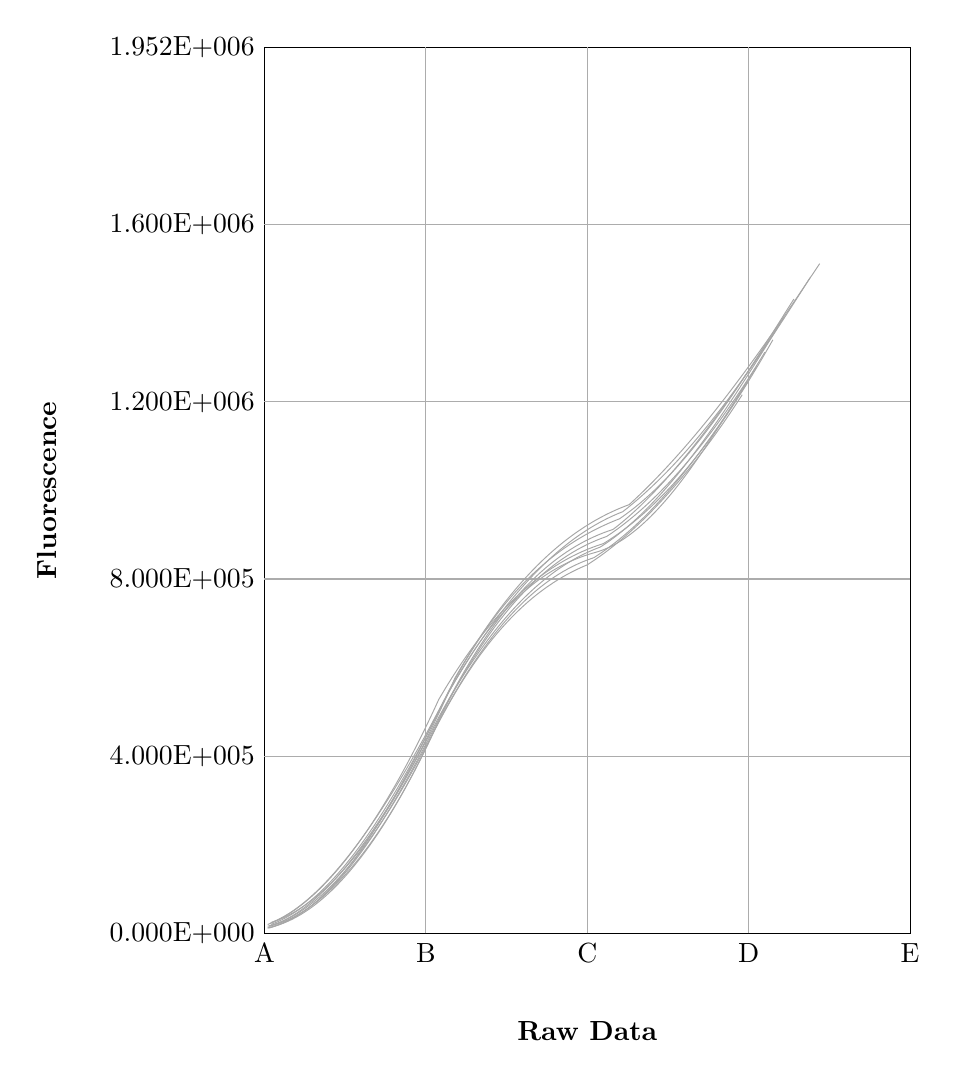
\begin{tikzpicture}[x=2.05cm,y=2.25cm]
  % Plot frame and grid
  \draw[black] (0,0) rectangle (4,5);
  \foreach \y in {1,2,3,4} {
    \draw[gray!65] (0,\y) -- (4,\y);
  }
  \foreach \x in {1,2,3} {
    \draw[gray!65] (\x,0) -- (\x,5);
  }

  % Fluorescence traces
  \draw[gray!70,line width=.35pt] (0.02,.03) .. controls (.35,.10) and (.65,.45) .. (1.05,1.20)
    .. controls (1.35,1.75) and (1.65,2.05) .. (2.05,2.15)
    .. controls (2.45,2.25) and (2.80,2.85) .. (3.05,3.20);

  \draw[gray!70,line width=.35pt] (0.02,.05) .. controls (.35,.16) and (.72,.60) .. (1.08,1.32)
    .. controls (1.42,1.85) and (1.75,2.10) .. (2.10,2.20)
    .. controls (2.55,2.45) and (2.90,2.95) .. (3.15,3.35);

  \draw[gray!70,line width=.35pt] (0.03,.04) .. controls (.40,.12) and (.70,.52) .. (1.12,1.28)
    .. controls (1.48,1.92) and (1.82,2.18) .. (2.16,2.28)
    .. controls (2.55,2.55) and (2.95,3.10) .. (3.22,3.48);

  \draw[gray!70,line width=.35pt] (0.04,.06) .. controls (.38,.18) and (.76,.68) .. (1.16,1.40)
    .. controls (1.50,1.98) and (1.86,2.22) .. (2.20,2.34)
    .. controls (2.65,2.62) and (3.00,3.18) .. (3.28,3.58);

  \draw[gray!70,line width=.35pt] (0.03,.03) .. controls (.42,.14) and (.78,.58) .. (1.10,1.24)
    .. controls (1.46,1.88) and (1.80,2.14) .. (2.12,2.24)
    .. controls (2.52,2.48) and (2.86,2.92) .. (3.10,3.28);

  \draw[gray!70,line width=.35pt] (0.02,.04) .. controls (.34,.11) and (.68,.48) .. (1.06,1.16)
    .. controls (1.38,1.72) and (1.70,2.02) .. (2.04,2.12)
    .. controls (2.44,2.35) and (2.76,2.78) .. (3.00,3.12);

  \draw[gray!70,line width=.35pt] (0.04,.05) .. controls (.40,.17) and (.74,.62) .. (1.14,1.36)
    .. controls (1.52,1.96) and (1.88,2.26) .. (2.22,2.38)
    .. controls (2.70,2.72) and (3.10,3.30) .. (3.38,3.70);

  \draw[gray!70,line width=.35pt] (0.03,.04) .. controls (.36,.13) and (.70,.55) .. (1.08,1.22)
    .. controls (1.44,1.82) and (1.78,2.08) .. (2.08,2.18)
    .. controls (2.50,2.42) and (2.88,2.98) .. (3.18,3.42);

  \draw[gray!70,line width=.35pt] (0.02,.03) .. controls (.38,.10) and (.72,.50) .. (1.04,1.12)
    .. controls (1.36,1.70) and (1.68,1.96) .. (2.00,2.08)
    .. controls (2.38,2.30) and (2.72,2.70) .. (2.96,3.04);

  \draw[gray!70,line width=.35pt] (0.04,.06) .. controls (.44,.18) and (.80,.66) .. (1.18,1.44)
    .. controls (1.54,2.02) and (1.90,2.30) .. (2.26,2.42)
    .. controls (2.74,2.82) and (3.16,3.40) .. (3.44,3.78);

  % Axis labels and ticks
  \node[below] at (0,0) {A};
  \node[below] at (1,0) {B};
  \node[below] at (2,0) {C};
  \node[below] at (3,0) {D};
  \node[below] at (4,0) {E};

  \node[left] at (0,0) {$0.000\mathrm{E}{+000}$};
  \node[left] at (0,1) {$4.000\mathrm{E}{+005}$};
  \node[left] at (0,2) {$8.000\mathrm{E}{+005}$};
  \node[left] at (0,3) {$1.200\mathrm{E}{+006}$};
  \node[left] at (0,4) {$1.600\mathrm{E}{+006}$};
  \node[left] at (0,5) {$1.952\mathrm{E}{+006}$};

  \node[below=1.0cm] at (2,0) {\textbf{Raw Data}};
  \node[rotate=90] at (-1.35,2.5) {\textbf{Fluorescence}};
\end{tikzpicture}
\end{center}

% TODO: The page header/footer metadata is partially illegible in the source image.
% LEXOID_PAGE_COMPLETED: 54/81

\newpage

\noindent
\begin{minipage}{\linewidth}
\small
Selected Detector: All \hfill M(Win): A1.2
\end{minipage}

% #VALUE_ID: LEX-P0055-V0001
% #TODO #HANDWRITTEN: [illegible signature]; blue handwritten characters
\handwritten{[illegible signature]}

% #VALUE_ID: LEX-P0055-V0002
% #TODO #HANDWRITTEN: 2025.9.01; handwritten date, partially unclear
\handwritten{2025.9.01}

% #VALUE_ID: LEX-P0055-V0003
% #TODO #HANDWRITTEN: [illegible initials or signature]; blue handwritten characters
\handwritten{[illegible initials or signature]}

% #VALUE_ID: LEX-P0055-V0004
% #TODO #HANDWRITTEN: 2025.9.02; handwritten date, partially unclear
\handwritten{2025.9.02}

\begin{center}
\textbf{Delta Rn vs Cycle}
\end{center}

\begin{figure}[ht]
\centering
% TODO: Insert the visible Delta Rn versus Cycle Number graph from this page.
% The graph contains multiple rising curves, a horizontal grid, Cycle Number
% values approximately 1--39 on the horizontal axis, and Delta Rn scientific-
% notation tick labels on the vertical axis.
\fbox{%
\begin{minipage}[c][0.63\textheight][c]{0.88\linewidth}
\centering
\textit{Graph: Delta Rn vs Cycle}\\[1ex]
\textit{Multiple plotted curves with gridlines}\\[1ex]
\textit{Horizontal axis: Cycle Number}\\
\textit{Vertical axis: Delta Rn}
\end{minipage}}
\caption*{Delta Rn versus Cycle Number}
\end{figure}

\noindent
\hfill Page 5 of 5\hfill
% LEXOID_PAGE_COMPLETED: 55/81

\newpage

\begin{center}
\textbf{艾米迈托莨注射液放行批检验记录}
\end{center}

\begin{center}
\small
\begin{tabular}{|p{2.3cm}|p{4.0cm}|p{2.3cm}|p{4.0cm}|}
\hline
\multicolumn{4}{|c|}{人细小病毒 B19 检验}\\
\hline
样品名称 &
\fieldvalue{艾米迈托莨注射液} &
样品规格 &
\fieldvalue{12mg：6.0$\times$10^{?} 个细胞}\\
\hline
样品批号 &
% #VALUE_ID: LEX-P0056-V0001
% #FIELD_VALUE: 样品批号
% #TODO #HANDWRITTEN: A?2??088?; handwriting unclear
\fieldvalue{\handwritten{A?2??088?}} &
取样日期 &
% #VALUE_ID: LEX-P0056-V0002
% #FIELD_VALUE: 取样日期
% #TODO #HANDWRITTEN: 202?年6月?日; handwriting unclear
\fieldvalue{\handwritten{202?年6月?日}}\\
\hline
\end{tabular}
\end{center}

\section{仪器设备及试剂}

\subsection{仪器设备}

\small
\begin{tabular}{|p{2.5cm}|p{2.0cm}|p{2.8cm}|p{2.8cm}|p{2.8cm}|}
\hline
仪器名称 & 厂家 & 型号 & 设备编号 & 校准有效期\\
\hline
\fieldvalue{生物安全柜} &
\fieldvalue{Thermo} &
\fieldvalue{1384} &
% #VALUE_ID: LEX-P0056-V0003
% #FIELD_VALUE: 生物安全柜设备编号
% #TODO #HANDWRITTEN: 14?205; handwriting unclear
\fieldvalue{\handwritten{14?205}} &
% #VALUE_ID: LEX-P0056-V0004
% #FIELD_VALUE: 生物安全柜校准有效期
% #TODO #HANDWRITTEN: 2021.02.12; handwriting unclear
\fieldvalue{\handwritten{2021.02.12}}\\
\hline
实时荧光定量 PCR 仪 &
\fieldvalue{Thermo} &
\fieldvalue{7500} &
% #VALUE_ID: LEX-P0056-V0005
% #FIELD_VALUE: 实时荧光定量 PCR 仪设备编号
% #TODO #HANDWRITTEN: 14?210; handwriting unclear
\fieldvalue{\handwritten{14?210}} &
% #VALUE_ID: LEX-P0056-V0006
% #FIELD_VALUE: 实时荧光定量 PCR 仪校准有效期
% #TODO #HANDWRITTEN: 2026.03.26; handwriting unclear
\fieldvalue{\handwritten{2026.03.26}}\\
\hline
移液器 &
\fieldvalue{Eppendorf} &
% #VALUE_ID: LEX-P0056-V0007
% #FIELD_VALUE: 移液器型号
% #TODO #HANDWRITTEN: 20--100\,\textmu l; handwriting unclear
\fieldvalue{\handwritten{20--100\,\textmu l}}\\[-1mm]
&
&
% #VALUE_ID: LEX-P0056-V0008
% #FIELD_VALUE: 移液器型号
% #TODO #HANDWRITTEN: 0.5--10\,\textmu l; handwriting unclear
\fieldvalue{\handwritten{0.5--10\,\textmu l}}\\[-1mm]
&
&
% #VALUE_ID: LEX-P0056-V0009
% #FIELD_VALUE: 移液器型号
% #TODO #HANDWRITTEN: 2--20\,\textmu l; handwriting unclear
\fieldvalue{\handwritten{2--20\,\textmu l}} &
% #VALUE_ID: LEX-P0056-V0010
% #FIELD_VALUE: 移液器设备编号
% #TODO #HANDWRITTEN: D?9580; handwriting unclear
\fieldvalue{\handwritten{D?9580}}\\[-1mm]
&
&
&
% #VALUE_ID: LEX-P0056-V0011
% #FIELD_VALUE: 移液器设备编号
% #TODO #HANDWRITTEN: 075?5K; handwriting unclear
\fieldvalue{\handwritten{075?5K}}\\[-1mm]
&
&
&
% #VALUE_ID: LEX-P0056-V0012
% #FIELD_VALUE: 移液器设备编号
% #TODO #HANDWRITTEN: R?606?; handwriting unclear
\fieldvalue{\handwritten{R?606?}} &
% #VALUE_ID: LEX-P0056-V0013
% #FIELD_VALUE: 移液器校准有效期
% #TODO #HANDWRITTEN: 2026.07.??; handwriting unclear
\fieldvalue{\handwritten{2026.07.??}}\\[-1mm]
&
&
&
&
% #VALUE_ID: LEX-P0056-V0014
% #FIELD_VALUE: 移液器校准有效期
% #TODO #HANDWRITTEN: 2026.09.??; handwriting unclear
\fieldvalue{\handwritten{2026.09.??}}\\[-1mm]
&
&
&
&
% #VALUE_ID: LEX-P0056-V0015
% #FIELD_VALUE: 移液器校准有效期
% #TODO #HANDWRITTEN: 2026.09.11; handwriting unclear
\fieldvalue{\handwritten{2026.09.11}}\\
\hline
\end{tabular}

\subsection{试剂}

\begin{center}
\small
\begin{tabular}{|p{3.5cm}|p{2.5cm}|p{2.5cm}|p{2.5cm}|p{2.5cm}|}
\hline
试剂名称 & 厂家 & 货号 & 批号 & 有效期至\\
\hline
\fieldvalue{人细小病毒 B19 核酸检测试剂盒（PCR-荧光探针法）} &
\fieldvalue{达安基因} &
% #VALUE_ID: LEX-P0056-V0016
% #FIELD_VALUE: 试剂货号
% #HANDWRITTEN: D51188
\fieldvalue{\handwritten{D51188}} &
% #VALUE_ID: LEX-P0056-V0017
% #FIELD_VALUE: 试剂批号
% #HANDWRITTEN: 2401107
\fieldvalue{\handwritten{2401107}} &
% #VALUE_ID: LEX-P0056-V0018
% #FIELD_VALUE: 试剂有效期至
% #HANDWRITTEN: 2025.1.06
\fieldvalue{\handwritten{2025.1.06}}\\
\hline
\end{tabular}
\end{center}

\section{操作步骤}

\subsection*{PCR 试剂准备（试剂准备区）}

\begin{center}
\small
\begin{tabular}{|p{7.2cm}|p{5.8cm}|}
\hline
按比例（B19 PCR 反应液 A 17\textmu l+B19 PCR 反应液 B 3\textmu l）取相应量的 PCR 反应液，充分混匀后，按 20\textmu l/管分装置 B19 PCR 反应液 & 
B19 PCR 反应液 A 体积 \\
&
% #VALUE_ID: LEX-P0056-V0019
% #FIELD_VALUE: B19 PCR 反应液 A 体积
% #HANDWRITTEN: 136
\fieldvalue{\handwritten{136}}\,\textmu l\\
\cline{2-2}
&
B19 PCR 反应液 B 体积 \\
&
% #VALUE_ID: LEX-P0056-V0020
% #FIELD_VALUE: B19 PCR 反应液 B 体积
% #HANDWRITTEN: 40
\fieldvalue{\handwritten{40}}\,\textmu l\\
\cline{2-2}
&
反应管加入混合液体积：\\
&
% #VALUE_ID: LEX-P0056-V0021
% #FIELD_VALUE: 反应管加入混合液体积
% #HANDWRITTEN: 20
\fieldvalue{\handwritten{20}}\,\textmu l\\
\hline
应管备用 & \\
\hline
\multicolumn{2}{|c|}{加样（样本制备区）}\\
\hline
往上述 B19 反应管中分别加入提取后的待测样本核酸、阴性质控品核酸、B19 阳性质控品核酸 5\textmu l。质控品 2 复孔，待测样品 3 复孔。 &
加入待测样本核酸、阴性质控品核酸、B19 阳性质控品核酸体积：\\
&
% #VALUE_ID: LEX-P0056-V0022
% #FIELD_VALUE: 加入核酸体积
% #HANDWRITTEN: 2
\fieldvalue{\handwritten{2}}\,\textmu l\\
&
质控品：\\
&
% #VALUE_ID: LEX-P0056-V0023
% #FIELD_VALUE: 质控品复孔数
% #HANDWRITTEN: 2
\fieldvalue{\handwritten{2}} 孔，待测样品\\
&
% #VALUE_ID: LEX-P0056-V0024
% #FIELD_VALUE: 待测样品复孔数
% #HANDWRITTEN: 3
\fieldvalue{\handwritten{3}} 孔\\
\hline
\multicolumn{2}{|c|}{PCR 扩增（扩增与分析区）}\\
\hline
\begin{tabular}{@{}p{5.5cm}@{}}
探针检测模式设置\\
（Target1: B19，Reporter Dye1: FAM，Quencher Dye1: None，Passive Reference: None。）
\end{tabular}
&
\begin{tabular}{@{}p{5.0cm}@{}}
Target 1 设置：\\
% #VALUE_ID: LEX-P0056-V0025
% #FIELD_VALUE: Target 1 设置
% #HANDWRITTEN: B19
\fieldvalue{\handwritten{B19}}\\
Reporter Dye 设置：\\
% #VALUE_ID: LEX-P0056-V0026
% #FIELD_VALUE: Reporter Dye 设置
% #HANDWRITTEN: FAM
\fieldvalue{\handwritten{FAM}}\\
Quencher Dye 设置：\\
% #VALUE_ID: LEX-P0056-V0027
% #FIELD_VALUE: Quencher Dye 设置
% #HANDWRITTEN: None
\fieldvalue{\handwritten{None}}\\
Passive Reference 设置：\\
% #VALUE_ID: LEX-P0056-V0028
% #FIELD_VALUE: Passive Reference 设置
% #HANDWRITTEN: None
\fieldvalue{\handwritten{None}}
\end{tabular}\\
\hline
\end{tabular}
\end{center}

% TODO: 页面底部显示“第72页 共73页”；页码及固定页脚未作为可编辑表单值转换。
% LEXOID_PAGE_COMPLETED: 56/81

\newpage

\begin{center}
\textbf{恒生生物科技（北京）有限公司}\\
\textit{PLATFORM LIFE SCIENCE TECHNOLOGY (BEIJING) CO., LTD.}\\[2mm]
\textbf{文件编号：REC-YZ-SOP-OC-03-092-}
\end{center}

\begin{tabular}{|p{0.22\linewidth}|p{0.12\linewidth}|p{0.16\linewidth}|p{0.16\linewidth}|p{0.16\linewidth}|}
\hline
扩增反应（50℃ 2分钟，1个循环；95℃ 15分钟，1个循环；94℃ 15秒$\rightarrow$55℃ 45秒（收集荧光），40个循环）
&
Stage 1
&
% #VALUE_ID: LEX-P0057-V0001
% #FIELD_VALUE: Stage 1 温度
% #HANDWRITTEN: 90
\fieldvalue{\handwritten{90}} ℃
&
% #VALUE_ID: LEX-P0057-V0002
% #FIELD_VALUE: Stage 1 时间
% #HANDWRITTEN: 2
\fieldvalue{\handwritten{2}} min
&
% #VALUE_ID: LEX-P0057-V0003
% #FIELD_VALUE: Stage 1 循环数
% #HANDWRITTEN: 1
\fieldvalue{\handwritten{1}} cycle
\\ \hline
&
Stage 2
&
% #VALUE_ID: LEX-P0057-V0004
% #FIELD_VALUE: Stage 2 温度
% #HANDWRITTEN: 95
\fieldvalue{\handwritten{95}} ℃
&
% #VALUE_ID: LEX-P0057-V0005
% #FIELD_VALUE: Stage 2 时间
% #HANDWRITTEN: 15
\fieldvalue{\handwritten{15}} min
&
% #VALUE_ID: LEX-P0057-V0006
% #FIELD_VALUE: Stage 2 循环数
% #HANDWRITTEN: 1
\fieldvalue{\handwritten{1}} cycle
\\ \hline
&
Stage 2
&
% #VALUE_ID: LEX-P0057-V0007
% #FIELD_VALUE: Stage 2 温度
% #HANDWRITTEN: 94
\fieldvalue{\handwritten{94}} ℃
&
% #VALUE_ID: LEX-P0057-V0008
% #FIELD_VALUE: Stage 2 时间
% #HANDWRITTEN: 15
\fieldvalue{\handwritten{15}} sec
&
% #VALUE_ID: LEX-P0057-V0009
% #FIELD_VALUE: Stage 2 循环数
% #HANDWRITTEN: 1
\fieldvalue{\handwritten{1}} cycle
\\ \hline
&
Stage 2
&
% #VALUE_ID: LEX-P0057-V0010
% #FIELD_VALUE: Stage 2 温度
% #HANDWRITTEN: 55
\fieldvalue{\handwritten{55}} ℃
&
% #VALUE_ID: LEX-P0057-V0011
% #FIELD_VALUE: Stage 2 时间
% #HANDWRITTEN: 45
\fieldvalue{\handwritten{45}} sec（收集荧光）
&
% #VALUE_ID: LEX-P0057-V0012
% #FIELD_VALUE: Stage 2 循环数
% #HANDWRITTEN: 40
\fieldvalue{\handwritten{40}} cycle
\\ \hline
\end{tabular}

\vspace{1mm}

\begin{tabular}{|p{0.22\linewidth}|p{0.70\linewidth}|}
\hline
数据保存路径 &
% #VALUE_ID: LEX-P0057-V0013
% #FIELD_VALUE: 数据保存路径
% #TODO #HANDWRITTEN: 161?7101-陕?-PCR-BC-PY-2025-08; 部分字符难以辨认
\fieldvalue{\handwritten{161?7101-陕?-PCR-BC-PY-2025-08}}\\
\hline
附件名称 &
% #VALUE_ID: LEX-P0057-V0014
% #FIELD_VALUE: 附件名称
% #TODO #HANDWRITTEN: 202508?-01?-?; 手写内容部分难以辨认
\fieldvalue{\handwritten{202508?-01?-?}}\\
\hline
\multicolumn{2}{|c|}{质量控制}\\
\hline
阴性质控品：FAM检测源扩增曲线无对数增长曲线 Ct值无检出 &
% #VALUE_ID: LEX-P0057-V0015
% #FIELD_VALUE: 阴性质控品，是
% #HANDWRITTEN: checked
\fieldvalue{\handwritten{\checkboxfield{checked}}} 是
\quad
% #VALUE_ID: LEX-P0057-V0016
% #FIELD_VALUE: 阴性质控品，否
\fieldvalue{\checkboxfield{unchecked}} 否
\\
\hline
阳性质控品：FAM检测源扩增曲线有明显对数增长曲线，且Ct值$\leq$32 &
% #VALUE_ID: LEX-P0057-V0017
% #FIELD_VALUE: 阳性质控品，是
% #HANDWRITTEN: checked
\fieldvalue{\handwritten{\checkboxfield{checked}}} 是
\quad
% #VALUE_ID: LEX-P0057-V0018
% #FIELD_VALUE: 阳性质控品，否
\fieldvalue{\checkboxfield{unchecked}} 否
\\
\hline
\multicolumn{2}{|c|}{质量控制\quad
% #VALUE_ID: LEX-P0057-V0019
% #FIELD_VALUE: 质量控制，通过
% #HANDWRITTEN: checked
\fieldvalue{\handwritten{\checkboxfield{checked}}} 通过
\quad
% #VALUE_ID: LEX-P0057-V0020
% #FIELD_VALUE: 质量控制，不通过
\fieldvalue{\checkboxfield{unchecked}} 不通过}\\
\hline
\multicolumn{2}{|c|}{检测结果}\\
\hline
检测孔 & \hfill 1 \hfill \qquad 2 \hfill \qquad 3 \hfill\\
\hline
样品 Ct 值 &
% #VALUE_ID: LEX-P0057-V0021
% #FIELD_VALUE: 检测孔1样品Ct值
% #HANDWRITTEN: Undet
\fieldvalue{\handwritten{Undet}}
\hfill
% #VALUE_ID: LEX-P0057-V0022
% #FIELD_VALUE: 检测孔2样品Ct值
% #HANDWRITTEN: Undet
\fieldvalue{\handwritten{Undet}}
\hfill
% #VALUE_ID: LEX-P0057-V0023
% #FIELD_VALUE: 检测孔3样品Ct值
% #HANDWRITTEN: Undet
\fieldvalue{\handwritten{Undet}}
\\
\hline
检测样本 Ct值$>38$，无扩增曲线或Ct值检出为阴性；检测样本Ct值$\leq38$，且有明显的扩增曲线为阳性 &
% #VALUE_ID: LEX-P0057-V0024
% #FIELD_VALUE: 检测结果，阳性
\fieldvalue{\checkboxfield{unchecked}} 阳性
\quad
% #VALUE_ID: LEX-P0057-V0025
% #FIELD_VALUE: 检测结果，阴性
\fieldvalue{\checkboxfield{unchecked}} 阴性
\\
\hline
结果判定 &
% #VALUE_ID: LEX-P0057-V0026
% #FIELD_VALUE: 结果判定，合格
% #HANDWRITTEN: checked
\fieldvalue{\handwritten{\checkboxfield{checked}}} 合格
\quad
% #VALUE_ID: LEX-P0057-V0027
% #FIELD_VALUE: 结果判定，不合格
\fieldvalue{\checkboxfield{unchecked}} 不合格
\\
\hline
备注 &
% #VALUE_ID: LEX-P0057-V0028
% #FIELD_VALUE: 备注
% #HANDWRITTEN: /
\fieldvalue{\handwritten{/}}\\
\hline
实验人/日期 &
% #VALUE_ID: LEX-P0057-V0029
% #FIELD_VALUE: 实验人
% #TODO #HANDWRITTEN: 彭馨?; 姓名末字难以辨认
\fieldvalue{\handwritten{彭馨?}}
\quad
% #VALUE_ID: LEX-P0057-V0030
% #FIELD_VALUE: 实验日期
% #HANDWRITTEN: 2025.08.28
\fieldvalue{\handwritten{2025.08.28}}\\
\hline
复核人/日期 &
% #VALUE_ID: LEX-P0057-V0031
% #FIELD_VALUE: 复核人
% #TODO #HANDWRITTEN: 翟佳?; 姓名难以辨认
\fieldvalue{\handwritten{翟佳?}}
\quad
% #VALUE_ID: LEX-P0057-V0032
% #FIELD_VALUE: 复核日期
% #HANDWRITTEN: 2025.08.29
\fieldvalue{\handwritten{2025.08.29}}\\
\hline
\end{tabular}

\vfill
\begin{center}
第 73 页 共 73 页
\end{center}
% LEXOID_PAGE_COMPLETED: 57/81

\newpage

\section{qPCR Report}

\subsection{File}

\begin{description}
  \item[Print Date:] %
  % #VALUE_ID: LEX-P0058-V0001
  % #FIELD_VALUE: Print Date
  \fieldvalue{2025-08-29 16:45:03}

  \item[Print By:] %
  % #VALUE_ID: LEX-P0058-V0002
  % #FIELD_VALUE: Print By
  \fieldvalue{TWL}

  \item[Instrument Type:] %
  % #VALUE_ID: LEX-P0058-V0003
  % #FIELD_VALUE: Instrument Type
  \fieldvalue{LUV}

  \item[FQC Volume:] %
  % #VALUE_ID: LEX-P0058-V0004
  % #FIELD_VALUE: FQC Volume
  \fieldvalue{25.5 Standard Curve}
\end{description}

% #VALUE_ID: LEX-P0058-V0005
% #HANDWRITTEN: [illegible Chinese signature]
% #TODO #HANDWRITTEN: [illegible Chinese signature]; blue handwritten signature
\handwritten{[illegible Chinese signature]}

% #VALUE_ID: LEX-P0058-V0006
% #HANDWRITTEN: 2025.08.06
\handwritten{2025.08.06}

% #VALUE_ID: LEX-P0058-V0007
% #HANDWRITTEN: [illegible Chinese name]
% #TODO #HANDWRITTEN: [illegible Chinese name]; blue handwritten name is unclear
\handwritten{[illegible Chinese name]}

% #VALUE_ID: LEX-P0058-V0008
% #HANDWRITTEN: 2025.08.06
\handwritten{2025.08.06}

\subsection{Electronic Signatures}

No associated Electronic Signatures.

\subsection{Document Information}

\begin{description}
  \item[Run Date:] %
  % #VALUE_ID: LEX-P0058-V0009
  % #FIELD_VALUE: Run Date
  \fieldvalue{Thursday, August 28, 2025 15:46:40}

  \item[Last Modified:] %
  % #VALUE_ID: LEX-P0058-V0010
  % #FIELD_VALUE: Last Modified
  \fieldvalue{Thursday, August 28, 2025 14:25:20}

  \item[Instrument Type:] %
  % #VALUE_ID: LEX-P0058-V0011
  % #FIELD_VALUE: Instrument Type
  \fieldvalue{Applied Biosystems 7500 Real-Time PCR System}
\end{description}

% TODO: Instrument identifier is partially unclear in the source image.
% #VALUE_ID: LEX-P0058-V0012
% #FIELD_VALUE: Instrument identifier
\fieldvalue{A3120250806006}

\subsection{Thermal Profile}

\begin{center}
\small
\begin{tabular}{|p{0.10\linewidth}|p{0.18\linewidth}|p{0.14\linewidth}|p{0.14\linewidth}|p{0.16\linewidth}|p{0.18\linewidth}|}
\hline
\textbf{Stage} & \textbf{Temperature} & \textbf{Time} & \textbf{Repeat} & \textbf{Ramp Rate} & \textbf{Auto Increment} \\
\hline
% #VALUE_ID: LEX-P0058-V0013
% #FIELD_VALUE: Stage
\fieldvalue{1}
&
% #VALUE_ID: LEX-P0058-V0014
% #FIELD_VALUE: Temperature
\fieldvalue{50.0\,^{\circ}\mathrm{C}}
&
% #VALUE_ID: LEX-P0058-V0015
% #FIELD_VALUE: Time
\fieldvalue{2:00}
&
% #VALUE_ID: LEX-P0058-V0016
% #FIELD_VALUE: Repeat
\fieldvalue{1}
&
% #VALUE_ID: LEX-P0058-V0017
% #FIELD_VALUE: Ramp Rate
\fieldvalue{100}
&
\\
\hline
% #VALUE_ID: LEX-P0058-V0018
% #FIELD_VALUE: Stage
\fieldvalue{2}
&
% #VALUE_ID: LEX-P0058-V0019
% #FIELD_VALUE: Temperature
\fieldvalue{95.0\,^{\circ}\mathrm{C}}
&
% #VALUE_ID: LEX-P0058-V0020
% #FIELD_VALUE: Time
\fieldvalue{0:15}
&
% #VALUE_ID: LEX-P0058-V0021
% #FIELD_VALUE: Repeat
\fieldvalue{1}
&
% #VALUE_ID: LEX-P0058-V0022
% #FIELD_VALUE: Ramp Rate
\fieldvalue{100}
&
\\
\hline
% #VALUE_ID: LEX-P0058-V0023
% #FIELD_VALUE: Stage
\fieldvalue{3}
&
% #VALUE_ID: LEX-P0058-V0024
% #FIELD_VALUE: Temperature
\fieldvalue{94.0\,^{\circ}\mathrm{C}}
&
% #VALUE_ID: LEX-P0058-V0025
% #FIELD_VALUE: Time
\fieldvalue{0:15}
&
% #VALUE_ID: LEX-P0058-V0026
% #FIELD_VALUE: Repeat
\fieldvalue{40}
&
% #VALUE_ID: LEX-P0058-V0027
% #FIELD_VALUE: Ramp Rate
\fieldvalue{100}
&
\\
\hline
% #VALUE_ID: LEX-P0058-V0028
% #FIELD_VALUE: Stage
\fieldvalue{4}
&
% #VALUE_ID: LEX-P0058-V0029
% #FIELD_VALUE: Temperature
\fieldvalue{55.0\,^{\circ}\mathrm{C}}
&
% #VALUE_ID: LEX-P0058-V0030
% #FIELD_VALUE: Time
\fieldvalue{0:45}
&
% #VALUE_ID: LEX-P0058-V0031
% #FIELD_VALUE: Repeat
\fieldvalue{40}
&
% #VALUE_ID: LEX-P0058-V0032
% #FIELD_VALUE: Ramp Rate
\fieldvalue{100}
&
\\
\hline
\end{tabular}
\end{center}

\subsection{Analysis Methods}

\begin{description}
  \item[Delta Rn:] %
  % #VALUE_ID: LEX-P0058-V0033
  % #FIELD_VALUE: Delta Rn
  \fieldvalue{}

  \item[Analysis Method:] %
  % #VALUE_ID: LEX-P0058-V0034
  % #FIELD_VALUE: Analysis Method
  \fieldvalue{Standard Curve}

  \item[Data Collection:] %
  % #VALUE_ID: LEX-P0058-V0035
  % #FIELD_VALUE: Data Collection
  \fieldvalue{Stage 3, Step 2}
\end{description}

\subsection{Detection Settings}

\subsection{Instrument Information}

% TODO: The Detection Settings and Instrument Information sections are visible as headings,
% but no additional field content is visible on this page.
% LEXOID_PAGE_COMPLETED: 58/81

\newpage

\begin{center}
\textbf{Reporter}\qquad FAM
\hfill
\textbf{Quantifier}\qquad (none)
\hfill
\textbf{Threshold}\qquad 1.95e+004
\hfill
\textbf{Baseline Start}\qquad 3
\hfill
\textbf{Baseline End}\qquad 15
\end{center}

\medskip

\small
\begin{tabular}{|p{0.06\linewidth}|p{0.23\linewidth}|p{0.14\linewidth}|p{0.14\linewidth}|p{0.08\linewidth}|p{0.08\linewidth}|p{0.09\linewidth}|p{0.09\linewidth}|p{0.09\linewidth}|p{0.08\linewidth}|p{0.08\linewidth}|}
\hline
\textbf{Well} &
\textbf{Sample Name} &
\textbf{Detector} &
\textbf{Type} &
\textbf{Cq} &
\textbf{Slope Cq} &
\textbf{Quantity} &
\textbf{Mean Qty} &
\textbf{Slope Qty} &
\textbf{Filtered} &
\textbf{Time}
\\ \hline
A1 & A3122202580800 B19 & Unknown & Undet. & & & & & & & \\
B1 & A3122202580800 B19 & Unknown & Undet. & & & & & & & \\
C1 & A3122202580800 B19 & Unknown & Undet. & & & & & & & \\
G1 & NC & Unknown & Undet. & & & & & & & \\
G12 & PC & B19 & Unknown & 0.086 & & & & & & \\
H12 & PC & B19 & Unknown & 22.783 & 0.086 & & & & & \\
\hline
\end{tabular}

\medskip

\noindent\texttt{20230828-319.sds}\hfill Page 2 of 4 (08/28/23 15:43:09)
% LEXOID_PAGE_COMPLETED: 59/81

\newpage

\begin{figure}[ht]
\centering
% TODO: Insert the graph image for this page; no source filename is available.
\fbox{\parbox[c][0.72\textheight][c]{0.88\linewidth}{\centering
\textbf{Fluorescence}\\[1em]
Graph with vertical fluorescence axis and horizontal raw-data axis.\\
Visible horizontal labels: A, B, C, D, E.\\
Visible plotted traces originate near the A region and extend toward the
upper portion of the graph.
}}
\caption{Fluorescence versus Raw Data}
\end{figure}

\noindent
\textit{Reading: 1}

\noindent
\textit{Wave(s): A--?}

\noindent
Page 34 (03/08/14 14:43:02)
% LEXOID_PAGE_COMPLETED: 60/81

\newpage

% TODO: The page is scanned upside down; content below is transcribed in its corrected reading orientation.

% #VALUE_ID: LEX-P0061-V0001
% #HANDWRITTEN: [illegible Chinese signature]
\handwritten{\text{[illegible Chinese signature]}}

% #VALUE_ID: LEX-P0061-V0002
% #HANDWRITTEN: 2025.08.08
\handwritten{2025.08.08}

% #VALUE_ID: LEX-P0061-V0003
% #HANDWRITTEN: [illegible Chinese signature]
\handwritten{\text{[illegible Chinese signature]}}

% #VALUE_ID: LEX-P0061-V0004
% #HANDWRITTEN: 2025.08.08
\handwritten{2025.08.08}

\hfill
\begin{tabular}{@{}ll@{}}
Selected Detector: &%
% #VALUE_ID: LEX-P0061-V0005
% #FIELD_VALUE: Selected Detector
\fieldvalue{All}\\
Wells: &%
% #VALUE_ID: LEX-P0061-V0006
% #FIELD_VALUE: Wells
\fieldvalue{A1-H12}
\end{tabular}

\begin{center}
\textbf{Delta Rn vs Cycle}
\end{center}

\begin{center}
% TODO: Reproduce the visible line graph and grid. The graph shows Delta Rn
% versus Cycle Number, with cycles 1--39 and y-axis tick labels ranging
% approximately from $-8.0\mathrm{e}{+003}$ to $4.4\mathrm{e}{+005}$.
\fbox{\parbox[c][0.62\textheight][c]{0.88\linewidth}{%
\centering
\textit{Graphical plot visible on this page}\\[1em]
\textbf{Delta Rn}\\[0.5em]
\begin{tabular}{c}
$4.4\mathrm{e}{+005}$\\
$3.9\mathrm{e}{+005}$\\
$3.4\mathrm{e}{+005}$\\
$2.9\mathrm{e}{+005}$\\
$2.4\mathrm{e}{+005}$\\
$1.9\mathrm{e}{+005}$\\
$1.4\mathrm{e}{+005}$\\
$9.19\mathrm{e}{+004}$\\
$4.19\mathrm{e}{+004}$\\
$-8.0\mathrm{e}{+003}$
\end{tabular}\\[1em]
\hrulefill\\[-0.2em]
\scriptsize
1\quad 2\quad 3\quad 4\quad 5\quad 6\quad 7\quad 8\quad 9\quad
10\quad 11\quad 12\quad 13\quad 14\quad 15\quad 16\quad 17\quad
18\quad 19\quad 20\quad 21\quad 22\quad 23\quad 24\quad 25\quad
26\quad 27\quad 28\quad 29\quad 30\quad 31\quad 32\quad 33\quad
34\quad 35\quad 36\quad 37\quad 38\quad 39\\[-0.2em]
\textbf{Cycle Number}
}}
\end{center}
% LEXOID_PAGE_COMPLETED: 61/81

\newpage

\begin{flushright}
\textit{阅微基因}\\
\textit{microread}
\end{flushright}

\noindent
文件编号：
% #VALUE_ID: LEX-P0062-V0001
% #FIELD_VALUE: 文件编号
\fieldvalue{MRL-TR-05：2023}
\hfill
实施日期：
% #VALUE_ID: LEX-P0062-V0002
% #FIELD_VALUE: 实施日期
\fieldvalue{2023-07-13}
\hfill
人源细胞 STR 检验报告

\noindent
北京阅微基因科技有限公司
\hfill
报告编号：
% #VALUE_ID: LEX-P0062-V0003
% #FIELD_VALUE: 报告编号
\fieldvalue{X3B0425-00420}

\begin{center}
\begin{tabular}{|p{0.22\linewidth}|p{0.28\linewidth}|p{0.22\linewidth}|p{0.23\linewidth}|}
\hline
样品标记 &
% #VALUE_ID: LEX-P0062-V0004
% #FIELD_VALUE: 样品标记
\fieldvalue{A31Z2202508006} &
来样数量 &
% #VALUE_ID: LEX-P0062-V0005
% #FIELD_VALUE: 来样数量
\fieldvalue{1管} \\
\hline
样本编号 &
% #VALUE_ID: LEX-P0062-V0006
% #FIELD_VALUE: 样本编号
\fieldvalue{X3B0425-00420} &
样本类型 &
% #VALUE_ID: LEX-P0062-V0007
% #FIELD_VALUE: 样本类型
\fieldvalue{细胞悬液} \\
\hline
来样状态 &
% #VALUE_ID: LEX-P0062-V0008
% #FIELD_VALUE: 来样状态
\fieldvalue{溶液} &
收件日期 &
% #VALUE_ID: LEX-P0062-V0009
% #FIELD_VALUE: 收件日期
\fieldvalue{2025-08-27} \\
\hline
客户联系人 &
% #VALUE_ID: LEX-P0062-V0010
% #FIELD_VALUE: 客户联系人
\fieldvalue{安圆丽老师} &
检测日期 &
% #VALUE_ID: LEX-P0062-V0011
% #FIELD_VALUE: 检测日期
\fieldvalue{2025-08-27} \\
\hline
联系方式 &
% #VALUE_ID: LEX-P0062-V0012
% #FIELD_VALUE: 联系方式
\fieldvalue{15652727620} &
报告日期 &
% #VALUE_ID: LEX-P0062-V0013
% #FIELD_VALUE: 报告日期
\fieldvalue{2025-08-30} \\
\hline
\multicolumn{1}{|l|}{客户单位} &
\multicolumn{3}{l|}{%
% #VALUE_ID: LEX-P0062-V0014
% #FIELD_VALUE: 客户单位
\fieldvalue{柏年卓越生物科技（北京）有限公司}} \\
\hline
\end{tabular}
\end{center}

\noindent
检验依据：

\begin{enumerate}
\item Human Cell Line Authentication Standardization of Short Tandem Repeat (STR) Profiling ASN-0002，2021 年修订版；
\item 中华人民共和国国家标准 2020 年版三部生物制品通则，生物制品生产检定用动物细胞基质指南。
\end{enumerate}

\noindent
检验方法按照中华人民共和国 2020 年版三部生物制品通则进行。取客户送检的适量样品 DNA，采用基因扩增及质量控制，使用 Promega 公司的 PowerPlex 21 系统进行 STR 分型检测；采用 MicroreadTME2M1 ID System 扩增 20 个 STR 位点和 Amelogenin 性别鉴定位点，使用 ABI 3730xl 遗传分析仪进行 PCR 产物检测，使用 GeneMapperID-X 软件（Applied Biosystems）对检测结果进行分析，并与 ATCC、DSMZ 和 ExPASy 数据库进行比对\textsuperscript{1,2}。

\noindent
检验结果细胞提取 DNA 溶液或者 DNA 浓度质量合格，实验中阴性及阳性对照结果均正确，检测样品细胞 DNA 扩增图谱清晰，读峰能与 STR 位点和 Amelogenin 位点的基因分型结果相符。检验结果见附表 1，分型图谱见附表 1--5；多等位基因数量如下\textsuperscript{3}：

\begin{center}
\begin{tabular}{|p{0.38\linewidth}|p{0.42\linewidth}|}
\hline
多等位基因数量 & 多等位基因名称 \\
\hline
% #VALUE_ID: LEX-P0062-V0015
% #FIELD_VALUE: 多等位基因数量
\fieldvalue{0} &
% #VALUE_ID: LEX-P0062-V0016
% #FIELD_VALUE: 多等位基因名称
\fieldvalue{--} \\
\hline
\end{tabular}
\end{center}

\noindent
检验结论：

\medskip

\noindent
该细胞 DNA 进行细胞 STR 分型结果显示：

\begin{enumerate}
\item 检测样本来自人源细胞。
\item 该细胞与 ATCC 中 HCM-BROD-0221-C43；Cancer Model；Metastatic；Melanoma；Human 细胞的 13 个位点数据匹配率为 67\%。
\item 该细胞与 DSMZ 中 KY821A3 的 9 个位点的数据匹配率为 83.3\%。
\item 该细胞与 ExPASy 中 HAF 的 8 个 STR 位点的数据匹配率为 73.33\%。
\end{enumerate}

\noindent
结论说明：依据 ATCC ASN-0002-2021 标准，比较 13 个位点 STR 基因座时，匹配度大于 80\% 可能为同一来源；比较 8 个 STR 基因座时，匹配度大于 90\% 可能为同一来源。

\begin{center}
（此结果仅对本次检测试验负责，未经本机构批准，不得复制本报告（全文复制除外））
\end{center}

\begin{center}
第1页共11页
\end{center}

\noindent
实验室地址：北京市昌平区中关村科技园区白浮泉路 1 号院 1 号楼

\noindent
电话：010-89780598 传真：010-89780599 网站：www.microread.com 邮箱：report@microread.com
% LEXOID_PAGE_COMPLETED: 62/81

\newpage

\noindent
\begin{tabular}{@{}p{0.43\linewidth}p{0.28\linewidth}p{0.29\linewidth}@{}}
文件编号：
% #VALUE_ID: LEX-P0063-V0001
% #FIELD_VALUE: 文件编号
\fieldvalue{MRL-TR-05:2023}
&
实施日期：
% #VALUE_ID: LEX-P0063-V0002
% #FIELD_VALUE: 实施日期
\fieldvalue{2023-07-13}
&
人源细胞 STR 检验报告
\end{tabular}

\vspace{0.15em}

\noindent
北京阅微基因技术股份有限公司
\hfill
报告编号：
% #VALUE_ID: LEX-P0063-V0003
% #FIELD_VALUE: 报告编号
\fieldvalue{X3B0425-004220}

\vspace{2.5em}

\noindent
\begin{tabular}{@{}p{0.33\linewidth}p{0.33\linewidth}p{0.34\linewidth}@{}}
编制：
% #VALUE_ID: LEX-P0063-V0004
% #FIELD_VALUE: 编制
% #TODO #HANDWRITTEN: 马柳程; 签名笔迹部分字形不清
\fieldvalue{\handwritten{马柳程}}
&
审核：
% #VALUE_ID: LEX-P0063-V0005
% #FIELD_VALUE: 审核
% #HANDWRITTEN: 孙学锋
\fieldvalue{\handwritten{孙学锋}}
&
批准：
% #VALUE_ID: LEX-P0063-V0006
% #FIELD_VALUE: 批准
% #HANDWRITTEN: 孙学锋
\fieldvalue{\handwritten{孙学锋}}
\end{tabular}

\vspace{0.8em}

\begin{center}
北京阅微基因技术股份有限公司
\end{center}

\vfill

\begin{center}
第2页共11页

实验室地址：北京市昌平区中关村科技园区北清路1号院1号楼

电话：010-89780958 \quad 传真：010-89780959 \quad
网址：www.microread.com.cn \quad 邮箱：report1@microread.com
\end{center}
% LEXOID_PAGE_COMPLETED: 63/81

\newpage

\begin{center}
\small
文件编号：MRL-TR-05-2023 \hfill 实施日期：2023-07-13 \hfill 人源细胞 STR 检验报告\\
北京市微碱基因技术有限公司 \hfill 报告编号：X3B0425-004220
\end{center}

\noindent\textbf{附表1：数据库比对结果（展示匹配度最高的结果）：}

\begin{center}
\small
\begin{tabular}{p{0.16\linewidth}p{0.15\linewidth}p{0.18\linewidth}p{0.13\linewidth}p{0.28\linewidth}}
\hline
 & ATCC & DSMZ & EPASy & 检测样品\\
\hline
 & HCM-BROD-022 & & & \\
 & I-C43; Cancer & & & \\
细胞名称 & Model; & KY821A3 & HAF & A31Z2022508006\\
 & Metastatic; & & & \\
 & Melanoma; & & & \\
 & Human & & & \\
\hline
细胞编号 & PDM-281 & JCRB0105.1 & CVCL\_A9FX & X3B0425-004220\\
\hline
Amelogenin & X,Y & X, X & X & X \quad X\\
D5S818 & 11,12 & 9,10,11,12,13 & 11 & 11 \quad 13\\
D13S317 & 11,12 & 8,9,11,12 & 11,12 & 11 \quad 12\\
D7S820 & 9,11 & 11,12 & 9,11 & 9 \quad 11\\
D16S539 & 12,13 & 10,11,12,13 & 11 & 11 \quad 12\\
vWA & 14,15 & 14,17,18 & 17,19 & 14 \quad 19\\
TH01 & 6,9 & 7,9 & 7,8 & 7 \quad 9\\
TPOX & 8,11 & 8,11 & 8,11 & 8 \quad 11\\
CSF1PO & 10,11 & 10,12 & 10,11 & 10 \quad 13\\
D19S433 & / & - & 14.2 & 15.2\\
D21S11 & 28,30 & - & & 29 \quad 30\\
D18S51 & 15,17 & - & & 13 \quad 15\\
D6S1043 & / & / & & 11 \quad 20\\
D3S1358 & 17,19 & - & & 17 \quad 17\\
Penta D & / & - & & 8 \quad 14\\
D2S441 & / & / & & 11.3 \quad 12\\
D8S1179 & 12 & - & & 10 \quad 12\\
Penta E & / & - & & 16 \quad 21\\
D12S391 & / & / & & 17 \quad 24\\
D2S1338 & / & - & & 17 \quad 17\\
\hline
\end{tabular}
\end{center}

\begin{center}
\footnotesize
第3页共11页\\
实验室地址：北京市昌平区中关村科技园区生命科学园1号院1号楼\\
电话：010-89780958 传真：010-89780959 网址：www.microread.com.cn 邮箱：report1@microread.com
\end{center}
% LEXOID_PAGE_COMPLETED: 64/81

\newpage

\noindent
文件编号：%
% #VALUE_ID: LEX-P0065-V0001
% #FIELD_VALUE: 文件编号
\fieldvalue{MRL-TR-05:2023}
\hfill
实施日期：%
% #VALUE_ID: LEX-P0065-V0002
% #FIELD_VALUE: 实施日期
\fieldvalue{2023-07-13}
\hfill
人源细胞 STR 检验报告

\noindent
北京微量基因科技有限公司
\hfill
报告编号：%
% #VALUE_ID: LEX-P0065-V0003
% #FIELD_VALUE: 报告编号
\fieldvalue{X3B045-00420}

\medskip

\noindent
\begin{tabular}{|p{0.13\linewidth}|p{0.17\linewidth}|p{0.17\linewidth}|p{0.17\linewidth}|p{0.20\linewidth}|}
\hline
 & ATCC & DSMZ & ExPASy & 检测样品 \\
\hline
FGA &
% #VALUE_ID: LEX-P0065-V0004
% #FIELD_VALUE: FGA--ATCC
\fieldvalue{21,23,24} &
% #VALUE_ID: LEX-P0065-V0005
% #FIELD_VALUE: FGA--DSMZ
\fieldvalue{-} &
% #VALUE_ID: LEX-P0065-V0006
% #FIELD_VALUE: FGA--ExPASy
\fieldvalue{23} &
% #VALUE_ID: LEX-P0065-V0007
% #FIELD_VALUE: FGA--检测样品
\fieldvalue{24} \\
\hline
共有 STR 位点 &
% #VALUE_ID: LEX-P0065-V0008
% #FIELD_VALUE: 共有 STR 位点--ATCC
\fieldvalue{13} &
% #VALUE_ID: LEX-P0065-V0009
% #FIELD_VALUE: 共有 STR 位点--DSMZ
\fieldvalue{9} &
% #VALUE_ID: LEX-P0065-V0010
% #FIELD_VALUE: 共有 STR 位点--ExPASy
\fieldvalue{8} &
\\
\hline
点数 &
% #VALUE_ID: LEX-P0065-V0011
% #FIELD_VALUE: 点数
\fieldvalue{4} &
 & & \\
\hline
匹配度 &
% #VALUE_ID: LEX-P0065-V0012
% #FIELD_VALUE: 匹配度--ATCC
\fieldvalue{67\%} &
% #VALUE_ID: LEX-P0065-V0013
% #FIELD_VALUE: 匹配度--DSMZ
\fieldvalue{83.3\%} &
% #VALUE_ID: LEX-P0065-V0014
% #FIELD_VALUE: 匹配度--ExPASy
\fieldvalue{73.33\%} &
\\
\hline
匹配说明 &
% #VALUE_ID: LEX-P0065-V0015
% #FIELD_VALUE: 匹配说明--ATCC
\fieldvalue{不可能力为相同来源细胞，需进一步验证} &
% #VALUE_ID: LEX-P0065-V0016
% #FIELD_VALUE: 匹配说明--DSMZ
\fieldvalue{需进一步验证} &
% #VALUE_ID: LEX-P0065-V0017
% #FIELD_VALUE: 匹配说明--ExPASy
\fieldvalue{需进一步验证} &
\\
\hline
\end{tabular}

\bigskip

\noindent\textbf{检测说明：}

\begin{enumerate}
  \item 有效峰为真实的 PCR 条带，小峰和非特异性杂带在计算中忽略不计。

  \item 检测细胞的分型结果与常规 PCR ATCC 和 DSMZ 细胞库，及 ExPASy 数据库中收录的来自于 ATCC、DSMZ、JCRB、ECACC 和 Riken 等多个细胞数据库中超过十万种人源细胞系 STR 分型中的 STR 数据匹配，数据分别和参考数据库中的细胞株无匹配，或不符合格局中的 STR 数据匹配，数据都是同比对结果表格中分别数据展示形式为 NA，此类样本与各细胞库比对结果为空白。

  \item 依据 ANSI/ATCC ASN-0002-2021 标准，混合培养物和 MSI 阳性细胞系均可在一个或多个 STR 基因座中显示额外的 STR 等位基因。其原因可能是：MSI 改变 DNA 复制错误导致的等位基因漂移，或存在含有污染的其他人源细胞系的混合培养物。

  \item 待检细胞和数据库中比对结果跟共存的位点数量。在进行匹配度计算时，DSMZ 数据库计入共有的 A.Megomin 性位点数，ATCC 及 ExPASy 数据库不计入。

  \item ATCC，DSMZ 及 ExPASy 数据库的匹配度计算所选取的算法为 “Tanabe”
  （DOI=10.1148/jtci19981.18.4_329）：待测细胞拷所有匹配个数 $\times 2$／（待测细胞+数据库）所有的个数 $\times 100\%$。

  \item 匹配说明：依据 ASN-0002-2021 标准，细胞系的匹配度分为 0--59\%，为不同来源细胞；60--69\%之间，不太可能为相同来源细胞，需进一步验证；70--79\%之间，相关细胞系具有此范围内的分数的一个常见原因是细胞系的 MSI 不稳定，细胞身份需进一步验证；80--89\%之间，比该 13 个位点 STR 基因座可能为同一来源；比较 8 个 STR 基因座时，则匹配的截止分数应为 90\% 以上；比对 13 个位点以上基因座且匹配分数在 90--100\%之间，最有可能为同一来源细胞。

  \item 结果提示：本报告的检验结论与数据库比对结果仍依据各组细胞（数据库）库规定计算得出。可能存在各库间仅收可同一细胞系分型信息不同，导致匹配结果有差异的情况。此外，受匹配计算模型的算法限制（共有 STR 位点数越少，匹配到关系统越可能越低），非同源系（株）的人源待测样本也存在一定概率能匹配到具相关性细胞，针对该类样本，本报告中提供的比对结果仅供参考。

  \item 本实验结论判定依据行业标准或共识解读，仅可用于细胞系的检验检定。我司不对项目指
导其真实性和适用性负责。
\end{enumerate}

\bigskip

\noindent
实验室地址：北京市昌平区中关村科技园区自北岸北京 1 号院 1 号楼

\noindent
电话：010-89798059\quad 传真：010-89798059\quad 网址：www.microread.com\quad 邮箱：report@microread.com
% LEXOID_PAGE_COMPLETED: 65/81

\newpage

\noindent
\begin{flushleft}
\small
文件编号：
% #VALUE_ID: LEX-P0066-V0001
% #FIELD_VALUE: 文件编号
\fieldvalue{MRL-TR-05：2023}
\hfill
实施日期：
% #VALUE_ID: LEX-P0066-V0002
% #FIELD_VALUE: 实施日期
\fieldvalue{2023-07-13}
\hfill
人类细胞 STR 检验报告

北京微量基因技术股份有限公司
\hfill
报告编号：
% #VALUE_ID: LEX-P0066-V0003
% #FIELD_VALUE: 报告编号
\fieldvalue{X3B045-004220}
\end{flushleft}

\noindent
定用途以外的其他用途或解释免责声明。

\vfill

\begin{center}
\small
第5页共11页

实验室地址：北京市昌平区中关村科技园区昌平园北清路1号院1号楼

电话：010-89780958 \quad 传真：010-89780959 \quad
网址：www.microread.com.cn \quad 邮箱：report1@microread.com
\end{center}
% LEXOID_PAGE_COMPLETED: 66/81

\newpage

\begin{center}
\textbf{图 1：纠偏 A312250?050?8?6 STR 过程图}
\end{center}

% TODO: The page contains a four-panel STR process chart with multiple plotted traces,
% axes, legends, colored markers, and Chinese annotations. No source image filename
% is available; insert the page/chart image here for faithful reproduction.
\begin{center}
\fbox{\parbox{0.95\linewidth}{\centering
\textit{[Four-panel STR process chart]}
}}
\end{center}

\vfill

\noindent
文件编号：MRL-TR-05-2023 \qquad 报告编号：XG8245-002420

\noindent
% TODO: Several Chinese footer lines, contact details, and the website/email address
% are too small and rotated in the supplied page image for reliable transcription.
% LEXOID_PAGE_COMPLETED: 67/81

\newpage

\noindent 文档编号：MRL-TR-05：2023 \hfill 日期：2023-07-13\\
\noindent 实验室检测报告

\begin{center}
\textbf{附图2：ATCC细胞比较结果报告清单}
\end{center}

% TODO: Several column headings and cell entries are low-resolution and have been transcribed to the best of the available image.

\begin{center}
\scriptsize
\begin{tabular}{|p{0.055\linewidth}|p{0.075\linewidth}|p{0.19\linewidth}|p{0.11\linewidth}|p{0.055\linewidth}|p{0.055\linewidth}|p{0.055\linewidth}|p{0.055\linewidth}|p{0.055\linewidth}|p{0.055\linewidth}|p{0.055\linewidth}|p{0.055\linewidth}|p{0.055\linewidth}|}
\hline
\textbf{Add to\\Date} &
\textbf{ATCC\\number*} &
\textbf{Designation*} &
\textbf{DMS?} &
\textbf{D?S?} &
\textbf{D?S?} &
\textbf{D?S?} &
\textbf{D?S?} &
\textbf{TH?} &
\textbf{AM?} &
\textbf{TPOK?} &
\textbf{C?S?} &
\textbf{DMS?}\\
\hline
67.0 & POM-A-231 &
HCM-RD-022-LS-3 Center\\
Human Melanoma &
1112 & 911 & 1233 & 21435 & 69 & XY & 811 & 10111 & 1\\
\hline
64.0 & CR-2321 &
BCL-2 Lymphoma Human &
1123 & 69 & 1112 & 1419 & 7 & XY & 1111 & 10112 & 1\\
\hline
58.0 & C? 3582 &
M?H? Glioma\\
Adenocarcinoma Human &
11 & 10111 & 11 & 1417 & 7 & XY & 811 & 10112 & 1\\
\hline
57.0 & F?M?L-43 &
HCM-RD-049? Cancer Melanoma\\
Primary Glioblastoma Brain cell &
1123 & 21 & 911 & 2147 & 7 & XY & 11 & 10111 & 1\\
\hline
57.0 & POM-5-378 &
HCM-RD-059? C? Cancer\\
Melanoma cell &
1133 & 11 & 911 & 1447 & 7 & XY & 11 & 10141 & 1\\
\hline
57.0 & H?E-70 &
SK-HEP-1 Melanoma Human &
1133 & 942? & 1012 & 2468 & 6.9 & X & 11 & 10113 & 1\\
\hline
57.0 & CR-2465 &
HS-27? Bone Marrow Human &
12 & 12 & 11?2 & 2819 & 7.9 & XY & 8.11 & 10111 & 2\\
\hline
57.0 & C? 778 &
Vero cell line &
4 & 8?1 & 9?4 & 7449 & 7?6 & Y & 6?1 & 144? & 2\\
\hline
\end{tabular}
\end{center}

\noindent 电话：010-879?598? \quad 地址：北京经济技术开发区\\
\noindent 网址：www.microread.com.cn \quad 邮箱：report@microread.com
% LEXOID_PAGE_COMPLETED: 68/81

\newpage

\begin{center}
\textbf{附图3：ATCC细胞比较结果图第2部分分析图}
\end{center}

\noindent
\textbf{委托编号：}MRL-TR-05-2023
\hfill
\textbf{检测日期：}2023-07-13
\hfill
\textbf{报告编号：}X?8025-004220

\medskip

\begin{center}
\scriptsize
\begin{tabular}{p{3.0cm}*{14}{p{0.72cm}}}
\hline
\textbf{Station}
& \textbf{D3S1358}
& \textbf{D13S317}
& \textbf{D7S820}
& \textbf{D16S539}
& \textbf{D5S818}
& \textbf{vWA}
& \textbf{TH01}
& \textbf{AMEL1}
& \textbf{TPOX}
& \textbf{CSF1PO}
& \textbf{D8S1179}
& \textbf{D21S11}
& \textbf{D18S51}
& \textbf{FGA}
\\
\hline
12-CA3 Cancer Model
& 11,12 & 21,12 & 9,11 & 12,13 & 12,13
& 14,15 & 6,9 & XY & 8,11 & 10,11
& 17,19 & 28,30 & 12 & 21,23
\\
\multicolumn{1}{p{3.0cm}}{Cancer Model}
& 11,13 & 21,12 & 8,9 & 11,13 & 12,13
& 14,19 & 7 & XY & 10,11 & 10,12
& 14,18 & 29,30 & 14,16 & 22,24
\\
\multicolumn{1}{p{3.0cm}}{Cancer Model}
& 11 & 11 & 10,11 & 12 & 12
& 14,17 & 7,3 & XY & 8,11 & 10,12
& 16 & 28,30 & 13 & 23,24
\\
\multicolumn{1}{p{3.0cm}}{C-7 Cancer Model}
& 11,13 & 11,14 & 11 & 11,14 & 11,14
& 14,17 & 7 & XY & 11 & 10,11
& 17 & 28,29 & 11 & 23
\\
\multicolumn{1}{p{3.0cm}}{Cancer Model}
& 11,13 & 11,14 & 11 & 10,12 & 11,14
& 14,17 & 7 & XY & 11 & 10,11
& 17 & 28,29 & 14,16 & 23
\\
\multicolumn{1}{p{3.0cm}}{Breast cancer}
& 11,12 & 11,13 & 12 & 11,13 & 11,13
& 14,19 & 7,9 & X & 11 & 9,12
& 14,17 & 29,30 & 15,16 & 21,24
\\
\multicolumn{1}{p{3.0cm}}{Additional sample}
& 11,12 & 11,13 & 12 & 11,13 & 11,13
& 14,19 & 7,9 & Y & 11 & 9,12
& 14,17 & 29,30 & 15,16 & 21,24
\\
\hline
\end{tabular}
\end{center}

% TODO: The source page is rotated and several station names and genotype entries are too small to read reliably.
\medskip

\noindent
\textbf{检测说明：}本检测报告仅对送检样品负责。

\noindent
地址：深圳市盐田区北山工业区；电话：400-810-8799；网址：www.microread.com；邮箱：report@microread.com
% LEXOID_PAGE_COMPLETED: 69/81

\newpage

\begin{center}
\textbf{附图4：DMSZ细胞比例分析结果图}

\vspace{0.5em}

\textbf{STR Profile Search}

\small
\begin{tabular}{|p{2.2cm}|c|c|c|c|c|c|c|c|c|c|c|c|c|c|c|}
\hline
Sample & Gender & D8S1179 & D21S11 & D7S820 & CSF1PO & D3S1358 &
TH01 & D13S317 & D16S539 & D2S1338 & D19S433 & vWA & TPOX &
D18S51 & Amelogenin & FGA \\
\hline
样本 &  &  &  &  &  &  &  &  &  &  &  &  &  &  &  &  \\
\hline
样本 &  &  &  &  &  &  &  &  &  &  &  &  &  &  &  &  \\
\hline
样本 &  &  &  &  &  &  &  &  &  &  &  &  &  &  &  &  \\
\hline
样本 &  &  &  &  &  &  &  &  &  &  &  &  &  &  &  &  \\
\hline
样本 &  &  &  &  &  &  &  &  &  &  &  &  &  &  &  &  \\
\hline
样本 &  &  &  &  &  &  &  &  &  &  &  &  &  &  &  &  \\
\hline
样本 &  &  &  &  &  &  &  &  &  &  &  &  &  &  &  &  \\
\hline
样本 &  &  &  &  &  &  &  &  &  &  &  &  &  &  &  &  \\
\hline
样本 &  &  &  &  &  &  &  &  &  &  &  &  &  &  &  &  \\
\hline
样本 &  &  &  &  &  &  &  &  &  &  &  &  &  &  &  &  \\
\hline
样本 &  &  &  &  &  &  &  &  &  &  &  &  &  &  &  &  \\
\hline
样本 &  &  &  &  &  &  &  &  &  &  &  &  &  &  &  &  \\
\hline
样本 &  &  &  &  &  &  &  &  &  &  &  &  &  &  &  &  \\
\hline
样本 &  &  &  &  &  &  &  &  &  &  &  &  &  &  &  &  \\
\hline
样本 &  &  &  &  &  &  &  &  &  &  &  &  &  &  &  &  \\
\hline
样本 &  &  &  &  &  &  &  &  &  &  &  &  &  &  &  &  \\
\hline
样本 &  &  &  &  &  &  &  &  &  &  &  &  &  &  &  &  \\
\hline
样本 &  &  &  &  &  &  &  &  &  &  &  &  &  &  &  &  \\
\hline
\end{tabular}
\end{center}

% TODO: The allele values and individual sample identifiers in the dense table are too small to transcribe reliably from the provided page image.

\vfill

\begin{center}
\footnotesize
太平洋保险 MR.L.TR-05-2023 \quad 表单编号：2023-07-13\\
电话：010-87985959 \quad 地址：北京市海淀区\\
网址：www.microread.com \quad 邮箱：report@microread.com
\end{center}
% LEXOID_PAGE_COMPLETED: 70/81

\newpage

\begin{center}
\textbf{文档编号：MIRL-TR-05-023 \qquad 文档日期：2023-07-13}
\end{center}

\begin{center}
\textbf{图3：E-Rays细胞比较结果图}
\end{center}

\begin{center}
\scriptsize
% TODO: The source page is rotated and the table text is low-resolution; several identifiers and
% column headings below require verification against the original PDF.
\begin{tabular}{|p{1.55cm}|p{0.75cm}|p{0.45cm}|p{0.55cm}|p{0.55cm}|p{0.55cm}|p{0.55cm}|p{0.55cm}|p{0.55cm}|p{0.55cm}|p{0.55cm}|p{0.55cm}|p{0.55cm}|p{0.55cm}|p{0.55cm}|p{0.55cm}|p{0.55cm}|p{0.55cm}|}
\hline
\textbf{Accession ID} &
\textbf{Name} &
\textbf{Sex} &
\textbf{D3S1358} &
\textbf{vWA} &
\textbf{D16S539} &
\textbf{CSF1PO} &
\textbf{TPOX} &
\textbf{D8S1179} &
\textbf{D21S11} &
\textbf{D18S51} &
\textbf{D5S818} &
\textbf{D13S317} &
\textbf{D7S820} &
\textbf{D3S1358} &
\textbf{FGA} &
\textbf{AMEL} &
\textbf{TH01}
\\
\hline
CLC\_A? &
? &
? &
11,12 &
17,18 &
9,11 &
10,12 &
8,11 &
12,13 &
29,31 &
14,15 &
11,12 &
8,12 &
9,11 &
15,16 &
22,24 &
X,Y &
6,9
\\
\hline
CLC\_B? &
? &
? &
11,12 &
17,18 &
9,11 &
10,12 &
8,11 &
12,13 &
29,31 &
14,15 &
11,12 &
8,12 &
9,11 &
15,16 &
22,24 &
X,Y &
6,9
\\
\hline
CLC\_C? &
? &
? &
11,13 &
17,18 &
9,11 &
10,12 &
8,11 &
12,13 &
29,31 &
14,15 &
11,12 &
8,12 &
9,11 &
15,16 &
22,24 &
X,Y &
6,9
\\
\hline
CLC\_D? &
? &
? &
11,12 &
17,18 &
9,11 &
10,12 &
8,11 &
12,13 &
29,31 &
14,15 &
11,12 &
8,12 &
9,11 &
15,16 &
22,24 &
X,Y &
6,9
\\
\hline
CLC\_E? &
? &
? &
11,13 &
17,18 &
9,11 &
10,12 &
8,11 &
12,13 &
29,31 &
14,15 &
11,12 &
8,12 &
9,11 &
15,16 &
22,24 &
X,Y &
6,9
\\
\hline
CLC\_F? &
? &
? &
11,12 &
17,18 &
9,11 &
10,12 &
8,11 &
12,13 &
29,31 &
14,15 &
11,12 &
8,12 &
9,11 &
15,16 &
22,24 &
X,Y &
6,9
\\
\hline
CLC\_G? &
? &
? &
11,13 &
17,18 &
9,11 &
10,12 &
8,11 &
12,13 &
29,31 &
14,15 &
11,12 &
8,12 &
9,11 &
15,16 &
22,24 &
X,Y &
6,9
\\
\hline
CLC\_H? &
? &
? &
11,12 &
17,18 &
9,11 &
10,12 &
8,11 &
12,13 &
29,31 &
14,15 &
11,12 &
8,12 &
9,11 &
15,16 &
22,24 &
X,Y &
6,9
\\
\hline
CLC\_I? &
? &
? &
11,13 &
17,18 &
9,11 &
10,12 &
8,11 &
12,13 &
29,31 &
14,15 &
11,12 &
8,12 &
9,11 &
15,16 &
22,24 &
X,Y &
6,9
\\
\hline
CLC\_J? &
? &
? &
11,12 &
17,18 &
9,11 &
10,12 &
8,11 &
12,13 &
29,31 &
14,15 &
11,12 &
8,12 &
9,11 &
15,16 &
22,24 &
X,Y &
6,9
\\
\hline
CLC\_K? &
? &
? &
11,13 &
17,18 &
9,11 &
10,12 &
8,11 &
12,13 &
29,31 &
14,15 &
11,12 &
8,12 &
9,11 &
15,16 &
22,24 &
X,Y &
6,9
\\
\hline
\end{tabular}
\end{center}

\vspace{0.5em}

\noindent
备注：本页为检测结果表格，表格内容在下一页继续。 % TODO: Verify continuation and complete all low-resolution entries from the source PDF.

\begin{center}
\scriptsize
检测单位：广东医科大学法医物证司法鉴定所\\
电话：010-87980958 \qquad 网址：www.microread.com.cn \qquad 邮箱：report@microread.com
\end{center}
% LEXOID_PAGE_COMPLETED: 71/81

\newpage

\noindent
\textbf{微谱检测}\hfill
% TODO: The vertical header text is partially rotated and difficult to read in the source page.
报告日期：2023-07-13\quad 人员编制：ST\quad 检验报告

\vspace{0.4em}
\noindent
文件编号：MRL-TR-05：2023\hfill
江苏省微谱检测技术服务有限公司\quad 归档编号：X38025-00420

\noindent
\dotfill

\vfill

\noindent
\footnotesize
电话：010-87998595\quad
传真：010-87998596\quad
地址：北京市大兴区亦庄经济技术开发区\quad
邮箱：report@microread.com
% LEXOID_PAGE_COMPLETED: 72/81

\newpage

\begin{center}
\Large\textbf{人源细胞 STR 检验报告}
\end{center}

\noindent
\begin{tabular}{p{0.46\linewidth}p{0.46\linewidth}}
文件编号：
% #VALUE_ID: LEX-P0073-V0001
% #FIELD_VALUE: 文件编号
\fieldvalue{MRL-TR-05：2023}
&
实施日期：
% #VALUE_ID: LEX-P0073-V0002
% #FIELD_VALUE: 实施日期
\fieldvalue{2023-08-10}
\\
报告编号：
% #VALUE_ID: LEX-P0073-V0003
% #FIELD_VALUE: 报告编号
\fieldvalue{X3B0423-002573}
&
\\
\end{tabular}

\vspace{0.5em}

\noindent
\begin{tabular}{|p{0.23\linewidth}|p{0.25\linewidth}|p{0.23\linewidth}|p{0.21\linewidth}|}
\hline
样品标记 &
% #VALUE_ID: LEX-P0073-V0004
% #FIELD_VALUE: 样品标记
\fieldvalue{A31P2307007}
&
来样数量 &
% #VALUE_ID: LEX-P0073-V0005
% #FIELD_VALUE: 来样数量
\fieldvalue{1管}
\\ \hline
样本编号 &
% #VALUE_ID: LEX-P0073-V0006
% #FIELD_VALUE: 样本编号
\fieldvalue{X3B0423-002573}
&
样本类型 &
% #VALUE_ID: LEX-P0073-V0007
% #FIELD_VALUE: 样本类型
\fieldvalue{细胞悬液}
\\ \hline
样本状态 &
% #VALUE_ID: LEX-P0073-V0008
% #FIELD_VALUE: 样本状态
\fieldvalue{溶液}
&
收样日期 &
% #VALUE_ID: LEX-P0073-V0009
% #FIELD_VALUE: 收样日期
\fieldvalue{2023-08-06}
\\ \hline
客户联系人 &
% #VALUE_ID: LEX-P0073-V0010
% #FIELD_VALUE: 客户联系人
\fieldvalue{古建飞}
&
检测日期 &
% #VALUE_ID: LEX-P0073-V0011
% #FIELD_VALUE: 检测日期
\fieldvalue{2023-08-06}
\\ \hline
联系方式 &
% #VALUE_ID: LEX-P0073-V0012
% #FIELD_VALUE: 联系方式
\fieldvalue{17600083204}
&
报告日期 &
% #VALUE_ID: LEX-P0073-V0013
% #FIELD_VALUE: 报告日期
\fieldvalue{2023-08-09}
\\ \hline
\multicolumn{1}{|p{0.23\linewidth}|}{客户单位}
&
\multicolumn{3}{p{0.69\linewidth}|}{
% #VALUE_ID: LEX-P0073-V0014
% #FIELD_VALUE: 客户单位
\fieldvalue{航生卓越生物科技（北京）有限公司}
}
\\ \hline
\end{tabular}

\vspace{0.8em}

\noindent
检验依据：1. Human Cell Line Authentication Standardization of Short Tandem Repeat (STR) Profiling ASN-0002\quad 2021年修订版；

\noindent
2. 中华人民共和国药典 2020 年版三部生物制品通则---生物制品生产检定用动物细胞基质制备及质量控制。

\medskip

\noindent
检验方法按照中华人民共和国药典 2020 年版三部生物制品通则---生物制品生产检定用动物细胞基质制备及质量控制要求，取客户送检的适量检材提取 DNA，采用 MicroreaderTM21 ID System 扩增 20 个 STR 位点和 Amelogenin 性别鉴定，使用 ABI 3730xl 型遗传分析仪进行 PCR 产物检测，使用 GeneMapperID-X 软件（Applied Biosystems）对检测结果进行分析，并与 ATCC、DSMZ 和 ExPaSy 数据库进行比对\textsuperscript{1,2}。

\noindent
检验结果细胞提取 DNA 浓度或者 DNA 浓度质量合格，实验中阴性及阳性对照结果均正确，检测结果符合国家标准。该细胞的 STR 位点检测结果如下：

\begin{center}
\begin{tabular}{|p{0.30\linewidth}|p{0.52\linewidth}|}
\hline
多等位基因数量 & 多等位基因名称 \\
\hline
% #VALUE_ID: LEX-P0073-V0015
% #FIELD_VALUE: 多等位基因数量
\fieldvalue{0}
&
% #VALUE_ID: LEX-P0073-V0016
% #FIELD_VALUE: 多等位基因名称
\fieldvalue{---}
\\
\hline
\end{tabular}
\end{center}

\noindent
检验结论：

\medskip

\noindent
该细胞 DNA 进行细胞 STR 分型结果显示：

\begin{enumerate}
\item 检测样本来自人源细胞。
\item 该细胞与 ATCC 中 184BS Breast Epithelial Human 细胞的 9 个位点数据匹配率为 82\%。
\item 该细胞与 DSMZ 中 KY821A3 的 9 个位点的数据匹配率为 83.3\%。
\item 该细胞与 ExPASy 中 CLNH5.5 的 8 个 STR 位点的数据匹配率为 75.68\%。
\end{enumerate}

\noindent
结论说明：依据 ATCC ASN-0002-2021 标准，比较 13 个位点 STR 基因座时，匹配度大于 80\% 可能为同一来源；比较 8 个 STR 基因座时，匹配度大于 90\% 可能为同一来源。

\vspace{0.5em}

\begin{center}
（此结果仅对本次检材负责，未经本机构批准，不得复制本报告（全文复制除外））
\end{center}

\vfill

\begin{center}
第1页共9页

实验室地址：北京市昌平区中关村科技园区白浮泉北街1号院1号楼

电话：010-89780598\quad 传真：010-89780959\quad 网址：www.microread.com.cn\quad 邮箱：report1@microread.com
\end{center}
% LEXOID_PAGE_COMPLETED: 73/81

\newpage

\noindent
\textbf{文件编号：}%
% #VALUE_ID: LEX-P0074-V0001
% #FIELD_VALUE: 文件编号
\fieldvalue{MRL-TR-05：2023}
\hfill
\textbf{实施日期：}%
% #VALUE_ID: LEX-P0074-V0002
% #FIELD_VALUE: 实施日期
\fieldvalue{2023-08-10}
\hfill
人源细胞 STR 检验报告

\noindent
北京微赛基因科技股份有限公司
\hfill
\textbf{报告编号：}%
% #VALUE_ID: LEX-P0074-V0003
% #FIELD_VALUE: 报告编号
\fieldvalue{X3B0423-002573}

\vspace{0.5em}

\noindent
编制：%
% #VALUE_ID: LEX-P0074-V0004
% #FIELD_VALUE: 编制
% #TODO #HANDWRITTEN: 孙学佳; 签名笔迹部分不清晰
\fieldvalue{\handwritten{孙学佳}}
\hfill
审核：%
% #VALUE_ID: LEX-P0074-V0005
% #FIELD_VALUE: 审核
% #HANDWRITTEN: 李晓蝶
\fieldvalue{\handwritten{李晓蝶}}
\hfill
批准：%
% #VALUE_ID: LEX-P0074-V0006
% #FIELD_VALUE: 批准
% #TODO #HANDWRITTEN: 孙学？; 签名末字难以辨认
\fieldvalue{\handwritten{孙学？}}

\vspace{0.5em}

\noindent
北京微赛基因科技股份有限公司（蓝色印章）

\vfill

\begin{center}
\small
第2页共9页\\
实验室地址：北京市昌平区中关村科技园区区）第1号楼1号楼\\
电话：010-89780958 传真：010-89780959 网址：www.microread.com.cn 电子邮箱：report1@microread.com
\end{center}
% LEXOID_PAGE_COMPLETED: 74/81

\newpage

\noindent
文件编号：MRL-TR-05：2023 \hfill 签发日期：2023-08-10 \hfill 人类细胞 STR 检验报告

\noindent
北京德润?基因技术服务有限公司 \hfill 报告编号：X3B0243-002573

\begin{center}
\textbf{数据库比对结果（展示匹配度最高的结果）：}
\end{center}

\noindent
\begin{tabular}{|p{2.3cm}|p{2.3cm}|p{2.3cm}|p{2.3cm}|p{3.2cm}|}
\hline
 & ATCC & DSMZ & ExPASy & 检测样品 \\
\hline
细胞名称 & 184B5Breast & KY821A3 & CLNH5.5 & A3IP2300707 \\
\hline
细胞编号 & CRL-8799 & JCRB0105.1 & CVCL\_3665 & X3B0423-002573 \\
\hline
\end{tabular}

\vspace{0.3em}

\noindent
\begin{tabular}{|p{2.1cm}|p{2.0cm}|p{2.8cm}|p{2.8cm}|p{1.2cm}|p{1.2cm}|}
\hline
 & ATCC & DSMZ & ExPASy & \multicolumn{2}{c|}{检测样品} \\
\hline
Amelogenin & X & X, X & X,Y & X & X \\
\hline
D5S818 & 11 & 9, 10, 11, 12, 13 & 10,11,13 & 11 & 13 \\
\hline
D13S317 & 11 & 8, 9, 11, 12 & 11 & 11 & 12 \\
\hline
D7S820 & 9,11 & 11, 12 & 9,11 & 9 & 11 \\
\hline
D16S539 & 11,12 & 10, 11, 12, 13 & 9,11,12 & 11 & 12 \\
\hline
vWA & 18,19 & 14, 17, 18 & 14,17,19,20 & 14 & 19 \\
\hline
TH01 & 9,3 & 7, 9 & 6,7,8,9 & 7 & 9 \\
\hline
TPOX & 11 & 8, 11 & 8,11 & 8 & 11 \\
\hline
CSF1PO & 10 & 10,12 & 10,12 & 10 & 13 \\
\hline
D19S433 & - & - &  & 14.2 & 15.2 \\
\hline
D21S11 & - &  &  & 29 & 30 \\
\hline
D18S51 & / & - &  & 13 & 15 \\
\hline
D6S1043 & / & / &  & 11 & 20 \\
\hline
D3S1358 & / & - &  & 17 & 17 \\
\hline
Penta D & / & - &  & 8 & 14 \\
\hline
D2S441 &  & / &  & 11.3 & 12 \\
\hline
D8S1179 & / & - &  & 10 & 12 \\
\hline
Penta E & / & - &  & 16 & 21 \\
\hline
D12S391 & / & / &  & 17 & 24 \\
\hline
D2S1338 &  & - &  & 17 & 17 \\
\hline
FGA & / & - &  & 23 & 24 \\
\hline
\end{tabular}

\vspace{0.3em}

\noindent
\begin{tabular}{|p{3.5cm}|p{2.2cm}|p{2.2cm}|p{2.2cm}|}
\hline
共有 STR 位 & 9 & 9 & 8 \\
\hline
点数$^{4}$ &  &  &  \\
\hline
匹配度$^{5}$ & 82\% & 83.3\% & 75.68\% \\
\hline
\end{tabular}

\vfill

\begin{center}
第3页共9页

实验室地址：北京市昌平区中关村科技园区生命科学园1号院1号楼

电话：010-89780958 传真：010-89780959 网址：www.microread.com 邮箱：report1@microread.com
\end{center}

% TODO：页眉右上角含有公司标志；原图中的部分公司名称及编号字符较模糊。
% LEXOID_PAGE_COMPLETED: 75/81

\newpage

\begin{center}
\small
文件编号：
% #VALUE_ID: LEX-P0076-V0001
% #FIELD_VALUE: 文件编号
\fieldvalue{MRL-TR-05：2023}
\hspace{2cm}
实施日期：
% #VALUE_ID: LEX-P0076-V0002
% #FIELD_VALUE: 实施日期
\fieldvalue{2023-08-10}
\hspace{2cm}
人员抽组 STR 检验报告

报告编号：
% #VALUE_ID: LEX-P0076-V0003
% #FIELD_VALUE: 报告编号
\fieldvalue{2023-002573}

\vspace{0.5em}

\begin{tabular}{p{0.16\linewidth}p{0.20\linewidth}p{0.20\linewidth}p{0.20\linewidth}p{0.16\linewidth}}
\hline
 & ATCC & DSMZ & ExPASy & 检测样品 \\
\hline
匹配说明 &
% #VALUE_ID: LEX-P0076-V0004
% #FIELD_VALUE: ATCC匹配说明
\fieldvalue{需进一步验证} &
% #VALUE_ID: LEX-P0076-V0005
% #FIELD_VALUE: DSMZ匹配说明
\fieldvalue{需进一步验证} &
% #VALUE_ID: LEX-P0076-V0006
% #FIELD_VALUE: ExPASy匹配说明
\fieldvalue{需进一步验证} &
\\
\hline
\end{tabular}
\end{center}

\vspace{1em}

\textbf{检测说明：}

\begin{enumerate}
\item 有效峰为真实的 PCR 条带，小峰和非特异性条带在计算中忽略不计。

\item 检测细胞的分型结果与收录于 ATCC 和 DSMZ 细胞库，及 ExPASy 数据库中收录的来自于 ATCC、DSMZ、JCRB、ECACC 和 Riken 等多个细胞数据库中经过十万余细胞系 STR 分型中的 STR 数据匹配。在报告期间未收录于上述细胞库的细胞将无法匹配；人源不合格样本由于无法获得分型，故数据序列比对结果将不会显示；此外，匹配不合格与各细胞库比对结果为空白。

\item 依据 ANSI/ATCC、JCRB、ECACC 和 DSMZ 等多个细胞库中至少一个或多个 STR 基因座中至少示额外的 STR 等位基因。其原因可能是：MSI 或其他 DNA 复制错误导致的等位基因漂移，或存在含有污染的其他人源细胞系的混合培养物。

\item 特征细胞和数据库中比对中结果细胞共有的 STR 位点数量，ATCC 及 DSMZ 计入 Amelogenin 性别位点，ExPASy 数据库不计入。

\item ATCC 数据库的匹配算法为待测细胞和所有匹配细胞系的匹配个数／ATCC 所有的个数$\times 100\%$，DSMZ 及 ExPASy 数据库的匹配度计算所选取的算法为 “Tanabe”
\[
[\mathrm{DOI}=10.14118/j.issn.0418\text{-}0456.1981.04.329]
\]
待测细胞和所有匹配细胞系的匹配个数／（待测细胞数量$\times 2$／（待测细胞数+数据库）所有的个数$\times 100\%$。

\item 匹配说明：依据 ASN-0002-2021 标准，细胞系的匹配百分为 $0$--$59\%$ 时，为不同来源细胞；$60$--$69\%$ 之间，不太可能为相同来源细胞；若进一步验证，$70$--$79\%$ 之间，相关细胞系具有非同源的范围内的分裂的一个常见原因是细胞系的 MSI 不稳定，细胞身份尚需进一步验证；$80$--$89\%$ 之间，比被 $13$ 个位点 STR 基因座时可能为同一来源；比较 $8$ 个 STR 基因座时，则匹配的截止分数应为 $90\%$ 以上；$90$--$100\%$ 之间，最有可能为同一来源细胞。

\item 结果提示：本报告的检验结论与数据库比对结果仅依据报告细胞（数据）库规定计算得出。可能存在各库间收录的同一细胞系分型信息不同，导致匹配结果有差异的情况。此外，受匹配度计算模型的算法限制（共有 STR 位点数越少，匹配到无关细胞可能性越高），非细胞系（株）的 人源待测样本存在一定程度能匹配到其相类似细胞，针对比类样本，本报告中提供的比对结果仅供参考。

\item 本实验结果判定依行业标准或共识解读，仅可用于细胞系的检验鉴定。我司不对项目指定用途以外的其他用途或解释负责。
\end{enumerate}

\begin{center}
\small
第4页共9页
\end{center}

\begin{center}
\scriptsize
实验室地址：北京市昌平区中关村科技园区永丰产业园 1 号院 1 号楼

电话：010-89780958 传真：010-89780959 网站：www.microread.com 邮箱：report01@microread.com
\end{center}
% LEXOID_PAGE_COMPLETED: 76/81

\newpage

\begin{center}
\textbf{太阳能电池组件 IV 测试报告}
\end{center}

\noindent
测试日期：2023-08-10

\noindent
附件 1：编号 A1327007 的 ST 诊断图

\vspace{1em}

\begin{center}
\begin{tabular}{c}
\fbox{\parbox[c][0.18\textheight][c]{0.92\linewidth}{\centering
\textbf{组件 1}\\
IV 测试曲线及诊断结果\\
\vspace{0.5em}
% TODO：此处为页面中可见的第一幅 IV 曲线图；原图包含电压、电流坐标轴、
% 绿色状态条、浅蓝色参考线及若干测试标记。
}}\\[1em]
\fbox{\parbox[c][0.18\textheight][c]{0.92\linewidth}{\centering
\textbf{组件 2}\\
IV 测试曲线及诊断结果\\
\vspace{0.5em}
% TODO：此处为页面中可见的第二幅 IV 曲线图；原图包含电压、电流坐标轴、
% 绿色状态条、浅蓝色参考线及若干测试标记。
}}\\[1em]
\fbox{\parbox[c][0.18\textheight][c]{0.92\linewidth}{\centering
\textbf{组件 3}\\
IV 测试曲线及诊断结果\\
\vspace{0.5em}
% TODO：此处为页面中可见的第三幅 IV 曲线图；原图包含电压、电流坐标轴、
% 绿色状态条、浅蓝色参考线及若干测试标记。
}}\\[1em]
\fbox{\parbox[c][0.18\textheight][c]{0.92\linewidth}{\centering
\textbf{组件 4}\\
IV 测试曲线及诊断结果\\
\vspace{0.5em}
% TODO：此处为页面中可见的第四幅 IV 曲线图；原图包含电压、电流坐标轴、
% 绿色状态条、浅蓝色参考线及若干测试标记。
}}
\end{tabular}
\end{center}

\vfill

\noindent
% TODO：页面底部可见检测机构地址、联系电话、网址及电子邮箱等页脚信息；
% 原图文字方向为横向旋转，部分字符无法可靠辨识。
% LEXOID_PAGE_COMPLETED: 77/81

\newpage

\begin{center}
\textbf{附图2：ATCC细胞比对结果图}
\end{center}

\noindent
\textbf{Showing 1--4 of 4}

\noindent
\textbf{Show per page:}\\
% #VALUE_ID: LEX-P0078-V0001
% #FIELD_VALUE: Show per page
\fieldvalue{24}

\medskip

\begin{center}
\small
\begin{tabular}{p{1.45cm}p{1.65cm}p{4.15cm}*{13}{p{0.62cm}}}
\hline
\textbf{Add to Cart} &
\textbf{Catalog Number} &
\textbf{Description} &
\textbf{D3S1358} &
\textbf{D8S1179} &
\textbf{D21S11} &
\textbf{D18S51} &
\textbf{D5S818} &
\textbf{D13S317} &
\textbf{D7S820} &
\textbf{D16S539} &
\textbf{vWA} &
\textbf{TH01} &
\textbf{AMEL} &
\textbf{TPOX} &
\textbf{CSF1PO}
\\
\hline
\textbf{BLD} &
\textbf{[catalog number]} &
293T/17 (Human embryonic kidney) &
12 &
9 &
31 &
15 &
12 &
12 &
9 &
11 &
14 &
9.3 &
X &
31 &
10
\\
\textbf{STD} &
\textbf{[catalog number]} &
\textit{HCT-116} (Human colorectal carcinoma) &
12 &
11/13 &
31 &
17 &
13 &
11 &
9 &
11 &
17 &
7 &
X &
21 &
10/12
\\
\textbf{BLD} &
\textbf{[catalog number]} &
BT-474 (Human breast carcinoma) &
11/13 &
9 &
30 &
15 &
11/13 &
11/12 &
9 &
11/12 &
14/15 &
7 &
X/Y &
10/12 &
9/12
\\
\textbf{STD} &
\textbf{[catalog number]} &
Adult Normal Human &
12 &
9/11 &
30 &
14 &
13 &
13 &
12 &
13 &
14 &
9.3 &
X &
8 &
13
\\
\hline
\end{tabular}
\end{center}

\noindent
\textbf{ADD TO CART}\hspace{1cm}\textbf{EXPORT TO EXCEL}

\medskip

\noindent
\textbf{Disclaimer:}

\noindent
Reference to the data shown and the information contained within this page are strictly for information. ATCC encourages you to evaluate every responsibility to assess the accuracy of these data; no warranty, express or implied, is made by ATCC as to their accuracy.

\medskip

\noindent
\textbf{免责声明：}本页面所示数据及其中包含的信息仅供参考。ATCC建议用户自行评估这些数据的准确性；ATCC不对其准确性作任何明示或暗示的保证。

\medskip

\noindent
文件编号：MRL-TR-05-2023 \hfill 检验报告编号：2023-08-10 人类细胞 STR 鉴定报告

\noindent
电话：010-80789588 \hfill 网址：www.wicroatech.com \hfill 邮箱：report@wicroatech.com

% TODO: Several catalog numbers and portions of the table text are too small to read reliably in the source page; verify against the PDF image.
% LEXOID_PAGE_COMPLETED: 78/81

\newpage

\noindent
\textbf{文件编号：}MRL-TR-05-2023

\noindent
\textbf{实验日期：}2023-08-10

\begin{center}
\textbf{附图3：DSMZ细胞的检测结果图}
\end{center}

\begin{center}
\textbf{STR Profile Search}
\end{center}

\noindent
\textbf{说明：}本页为 DSMZ 细胞 STR 检测结果表。表格包含样本名称及多个 STR 位点的检测数据。

\vspace{0.5em}

\begin{center}
\scriptsize
\begin{tabular}{|p{2.2cm}|p{1.25cm}|p{1.25cm}|p{1.25cm}|p{1.25cm}|p{1.25cm}|p{1.25cm}|p{1.25cm}|p{1.25cm}|}
\hline
\textbf{Sample Name} &
\textbf{Amelogenin} &
\textbf{D8S1179} &
\textbf{D21S11} &
\textbf{D7S820} &
\textbf{CSF1PO} &
\textbf{D3S1358} &
\textbf{TH01} &
\textbf{D13S317}
\\ \hline
\textit{表格中的 DSMZ 细胞样本及对应 STR 检测数据} &
\multicolumn{8}{c|}{\textit{检测结果见原表}} 
\\ \hline
\end{tabular}
\end{center}

\vspace{0.5em}

\begin{center}
\scriptsize
\begin{tabular}{|p{1.25cm}|p{1.25cm}|p{1.25cm}|p{1.25cm}|p{1.25cm}|p{1.25cm}|p{1.25cm}|p{1.25cm}|p{1.25cm}|}
\hline
\textbf{D16S539} &
\textbf{D2S1338} &
\textbf{D19S433} &
\textbf{vWA} &
\textbf{TPOX} &
\textbf{D18S51} &
\textbf{D5S818} &
\textbf{FGA} &
\textbf{其他}
\\ \hline
\multicolumn{9}{c|}{\textit{本页表格中的具体数值分辨率不足，无法可靠辨识}}
\\ \hline
\end{tabular}
\end{center}

% TODO: 本页中央为一张多行 DSMZ 细胞 STR 检测结果表。由于当前页面图像分辨率及旋转方向导致表内样本名称和等位基因数值无法可靠逐项辨识；应使用原始 PDF 页面或高分辨率裁剪图补录全部可见表格内容。

\vfill

\noindent
\scriptsize
\textbf{联系方式：}电话、地址及电子邮箱信息位于页面底部；当前图像中具体字符无法可靠辨识。
% LEXOID_PAGE_COMPLETED: 79/81

\newpage

\begin{center}
\textbf{附件4\quad E+RAYS监测点站分布图}

\vspace{0.5em}

\small
\resizebox{\textwidth}{!}{%
\begin{tabular}{|c|l|c|c|c|c|c|c|c|c|c|c|c|c|c|c|c|c|}
\hline
序号 &
监测点名称 &
监测点编号 &
经度 &
纬度 &
海拔/m &
监测时间 &
监测项目 &
监测结果 &
\multicolumn{10}{c|}{监测数据} \\
\cline{10-19}
& & & & & & & &
& 1 & 2 & 3 & 4 & 5 & 6 & 7 & 8 & 9 & 10 \\
\hline
1  & CXCJ\_001 & \text{—} & \text{—} & \text{—} & \text{—} & \text{—} & \text{—} & \text{—} & \text{—} & \text{—} & \text{—} & \text{—} & \text{—} & \text{—} & \text{—} & \text{—} & \text{—} & \text{—} \\
\hline
2  & CXCJ\_002 & \text{—} & \text{—} & \text{—} & \text{—} & \text{—} & \text{—} & \text{—} & \text{—} & \text{—} & \text{—} & \text{—} & \text{—} & \text{—} & \text{—} & \text{—} & \text{—} & \text{—} \\
\hline
3  & CXCJ\_003 & \text{—} & \text{—} & \text{—} & \text{—} & \text{—} & \text{—} & \text{—} & \text{—} & \text{—} & \text{—} & \text{—} & \text{—} & \text{—} & \text{—} & \text{—} & \text{—} & \text{—} \\
\hline
4  & CXCJ\_004 & \text{—} & \text{—} & \text{—} & \text{—} & \text{—} & \text{—} & \text{—} & \text{—} & \text{—} & \text{—} & \text{—} & \text{—} & \text{—} & \text{—} & \text{—} & \text{—} & \text{—} \\
\hline
5  & CXCJ\_005 & \text{—} & \text{—} & \text{—} & \text{—} & \text{—} & \text{—} & \text{—} & \text{—} & \text{—} & \text{—} & \text{—} & \text{—} & \text{—} & \text{—} & \text{—} & \text{—} & \text{—} \\
\hline
6  & CXCJ\_006 & \text{—} & \text{—} & \text{—} & \text{—} & \text{—} & \text{—} & \text{—} & \text{—} & \text{—} & \text{—} & \text{—} & \text{—} & \text{—} & \text{—} & \text{—} & \text{—} & \text{—} \\
\hline
7  & CXCJ\_007 & \text{—} & \text{—} & \text{—} & \text{—} & \text{—} & \text{—} & \text{—} & \text{—} & \text{—} & \text{—} & \text{—} & \text{—} & \text{—} & \text{—} & \text{—} & \text{—} & \text{—} \\
\hline
8  & CXCJ\_008 & \text{—} & \text{—} & \text{—} & \text{—} & \text{—} & \text{—} & \text{—} & \text{—} & \text{—} & \text{—} & \text{—} & \text{—} & \text{—} & \text{—} & \text{—} & \text{—} & \text{—} \\
\hline
9  & CXCJ\_009 & \text{—} & \text{—} & \text{—} & \text{—} & \text{—} & \text{—} & \text{—} & \text{—} & \text{—} & \text{—} & \text{—} & \text{—} & \text{—} & \text{—} & \text{—} & \text{—} & \text{—} \\
\hline
10 & CXCJ\_010 & \text{—} & \text{—} & \text{—} & \text{—} & \text{—} & \text{—} & \text{—} & \text{—} & \text{—} & \text{—} & \text{—} & \text{—} & \text{—} & \text{—} & \text{—} & \text{—} & \text{—} \\
\hline
11 & CXCJ\_011 & \text{—} & \text{—} & \text{—} & \text{—} & \text{—} & \text{—} & \text{—} & \text{—} & \text{—} & \text{—} & \text{—} & \text{—} & \text{—} & \text{—} & \text{—} & \text{—} & \text{—} \\
\hline
12 & CXCJ\_012 & \text{—} & \text{—} & \text{—} & \text{—} & \text{—} & \text{—} & \text{—} & \text{—} & \text{—} & \text{—} & \text{—} & \text{—} & \text{—} & \text{—} & \text{—} & \text{—} & \text{—} \\
\hline
13 & CXCJ\_013 & \text{—} & \text{—} & \text{—} & \text{—} & \text{—} & \text{—} & \text{—} & \text{—} & \text{—} & \text{—} & \text{—} & \text{—} & \text{—} & \text{—} & \text{—} & \text{—} & \text{—} \\
\hline
14 & CXCJ\_014 & \text{—} & \text{—} & \text{—} & \text{—} & \text{—} & \text{—} & \text{—} & \text{—} & \text{—} & \text{—} & \text{—} & \text{—} & \text{—} & \text{—} & \text{—} & \text{—} & \text{—} \\
\hline
15 & CXCJ\_015 & \text{—} & \text{—} & \text{—} & \text{—} & \text{—} & \text{—} & \text{—} & \text{—} & \text{—} & \text{—} & \text{—} & \text{—} & \text{—} & \text{—} & \text{—} & \text{—} & \text{—} \\
\hline
\end{tabular}%
}
\end{center}

% TODO: The page contains a very small, rotated monitoring-data table. Individual station names, coordinates, dates, and numeric measurements are not reliably legible at the supplied resolution; the table structure and visibly discernible station identifiers are retained above.

\vfill

\begin{center}
\footnotesize
表格编号：2023-08-10\quad
\text{（相关项目及监测数据见表内）}
\end{center}
% LEXOID_PAGE_COMPLETED: 80/81

\newpage

\begin{center}
\rotatebox{90}{%
\begin{minipage}{0.92\textheight}
\small
文件编号：MRL-TR-05：2023 \qquad 实施日期：2023-08-10 \qquad
人员相关报告

\vfill

\begin{center}
\dotfill\quad 以下无正文 \quad\dotfill
\end{center}

\vfill

\begin{center}
电话：010-87985995 \qquad 传真：010-87985995\\
网址：www.microread.com \qquad 邮箱：report@microread.com
\end{center}

% TODO：页面边缘可见的机构标识及其余页脚文字过小且方向旋转，无法可靠辨识。
\end{minipage}%
}
\end{center}

\end{document}
% LEXOID_PAGE_COMPLETED: 81/81
